\part{Efeito dos aditivos hidrofílicos}
	\label{sec:efeito_aditivos_hidrofilicos} 

	\chapter{Resultados reológicos e calorimétricos}
		
	Esta é a parte principal desta tese, na qual houve uma dedicação prolongada. Aqui, pesquisou-se sobre efeitos dos aditivos hidrofílicos no comportamento das micelas gigantes. Parte dos resultados foram publicados na revista \emph{Journal of Colloid and Interface Science}, sob o título ``\emph{Rheological and calorimetric study of alkyltrimethylammonium bromide-sodium salicylate wormlike micelles in aqueous binary systems}"\cite{Clinckspoor2018}.
	
	A inspiração para a escolha da glicerina e do DMSO veio de estudos de outras áreas, onde se mostrou que ambos possuíam a capacidade de melhorar o armazenamento criogênico de células animais, como hemácias e esperma\cite{Butler1959, Polge1949}, sendo que essa propriedade do DMSO está relacionada à sua capacidade de permear membranas\cite{Notman2006}. Logo, se esses aditivos foram capazes de preservar células vivas após o congelamento, qual seria seu efeito em sistemas de autoassociação? Desse tipo de questionamento vieram os estudos de Hoffmann\cite{Grabner2014, Song2008a, Shinto2012}. Em seguida, \citeauthor{Abdel-Rahem2014} utilizou o 1,3-butanodiol, devido às suas aplicações como aditivo para fixar fragrâncias e agente antimicrobiano. A sacarose foi escolhida, devido à similaridade de suas interações com a água, e à similaridade da constante dielétrica, com a glicerina, e por já ter sido estudada anteriormente, com lamelas.\cite{Song2008a} Por último, a ureia é um aditivo frequentemente descrito como agente desestruturante da água, que leva à desnaturação de proteínas, aumenta a solubilidade de hidrocarbonetos e inibe a agregação micelar.\cite{Kuharski1984} Seguindo a hipótese de \citeauthor{Hoffmann2010}, esses aditivos, apesar de serem diferentes estruturalmente, deveriam resultar em efeitos nos perfis de viscosidade, e possivelmente nas outras técnicas, caso seus índices de refração sejam semelhantes. 
	
	Serão apresentados inicialmente os resultados de curva de fluxo (\autoref{sec:efeito_aditivos_viscosidade}). Em conjunto, serão apresentados os resultados calorimétricos, tanto de formação de micelas gigantes (\autoref{sec:efeito_aditivos_calorimetria_mg}) quanto de formação de micelas esféricas (\autoref{sec:efeito_aditivos_calorimetria_me}). Em seguida, serão levantados alguns parâmetros que podem ser utilizados para descrever o efeito dos aditivos (\autoref{sec:efeito_aditivos_viscosidade}). Os resultados calorimétricos serão correlacionados aos parâmetros (\autoref{sec:correlacao_params_cmc_dh}). Como complemento aos estudos com as curvas de fluxo, será avaliada a reologia oscilatória (\autoref{sec:reologia_oscilatoria}), e, como será mostrado, a ureia possui um efeito muito diferente, e será estudado mais a fundo no \autoref{sec:cap_efeito_ureia}.
	
	Como base para a discussão, utilizou-se a concentração dos aditivos em fração mássica (\% m/m). Isso se deve porque é a base de concentração utilizada na literatura da área, e os bancos de dados possuem as propriedades geralmente em função dessa grandeza. O \autoref{sec:tabelas_conversao} contém algumas tabelas convertendo a fração mássica para outras grandezas de concentração, como molaridade, molalidade, fração molar e proporções molares.

	
		\section{Efeitos dos aditivos na viscosidade do repouso} \index{resultados!efeito do solvente}
			\label{sec:efeito_aditivos_viscosidade} \index{resultados!índice de refração} \index{resultados!índice de refração}
			A reologia é uma técnica que pode fornecer informações sobre a dinâmica de relaxação de um material, através da viscosidade. Em especial, o perfil de viscosidade em repouso \(\eta_0\) (\autoref{fig:regioes_rh}) está relacionado com mudanças no processo de relaxação das micelas. Com o intuito de se estudar como a relaxação das micelas é afetada pelos aditivos, foram construídos vários diagramas de viscosidade, sempre com 100 \mM{} de \CTAB, para várias concentrações de aditivo.
			
			Neste momento, os resultados serão discutidos com base somente no índice de refração das soluções, partindo da primeira premissa apresentada na \autoref{sec:efeito_solvente}. Relembrando, essa premissa se baseia na diminuição no valor da constante de Hamaker (\autoref{eqn:constante_hamaker_lifshitz}), que diminui a atração entre as micelas, consequentemente acelerando o mecanismo de reptação, e não afetando o mecanismo de quebra e recombinação (\autoref{fig:regioes_rh}). A \autoref{fig:indice_refracao} mostra como o índice de refração das soluções com os aditivos variam em função da fração mássica de aditivo. A reta horizontal possui o mesmo índice de refração, então aditivos diferentes deveriam ter o mesmo efeito na reologia.
					
			\begin{figure}[h]
				\centering
				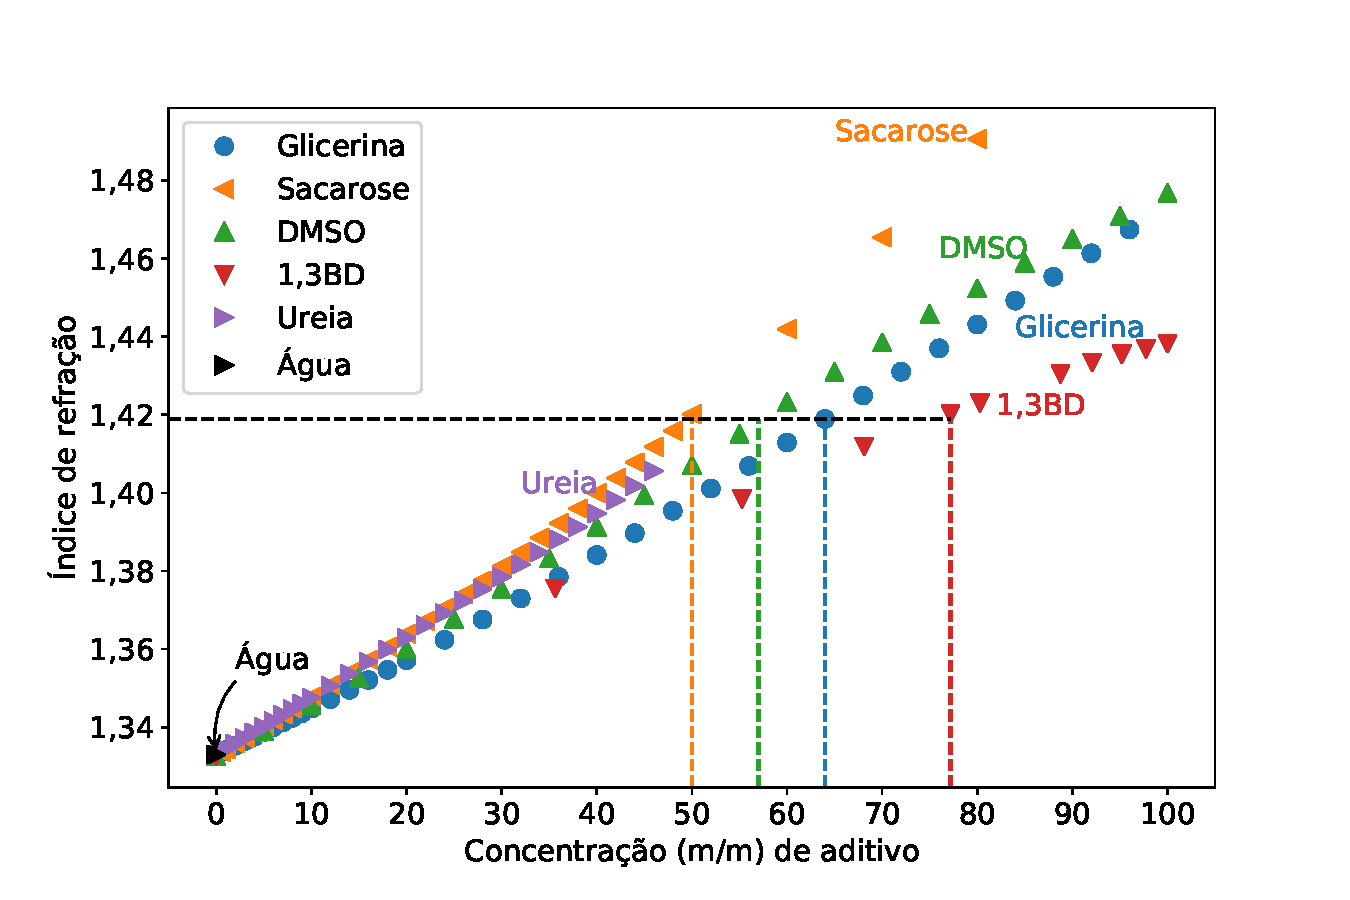
\includegraphics[width=0.7\textwidth]{imagens/propriedades/indice_refracao}
				\caption{Índice de refração  em função da concentração de glicerina, sacarose e ureia a 20°C\cite{Lide2003}, e de DMSO\cite{Lebel1962} e 1,3-butanodiol\cite{Piekarski1995} a 25°C. Na linha horizontal, as amostras dos aditivos teriam o mesmo índice de refração, e deveriam possuir o mesmo efeito na constante de Hamaker.}
				\label{fig:indice_refracao}
			\end{figure} \index{propriedades!índice de refração \(n\)}
	
			Inicialmente, comparou-se glicerina com sacarose, devido às suas semelhanças no índice de refração. A \autoref{fig:rh_sacarose_glicerina} mostra os diagramas de viscosidade, em concentrações crescentes de glicerina, e no ponto de igualdade no índice de refração de sacarose, 50\%. Em seguida, notou-se que \BD{} e DMSO possuiam efeitos semelhantes, como mostra a \autoref{fig:rh_13bd_dmso}. Por último, a ureia mostrou um comportamento muito diferente dos outros aditivos (\autoref{fig:rh_ureia}).
			
			\begin{figure}[htb]
				\centering
				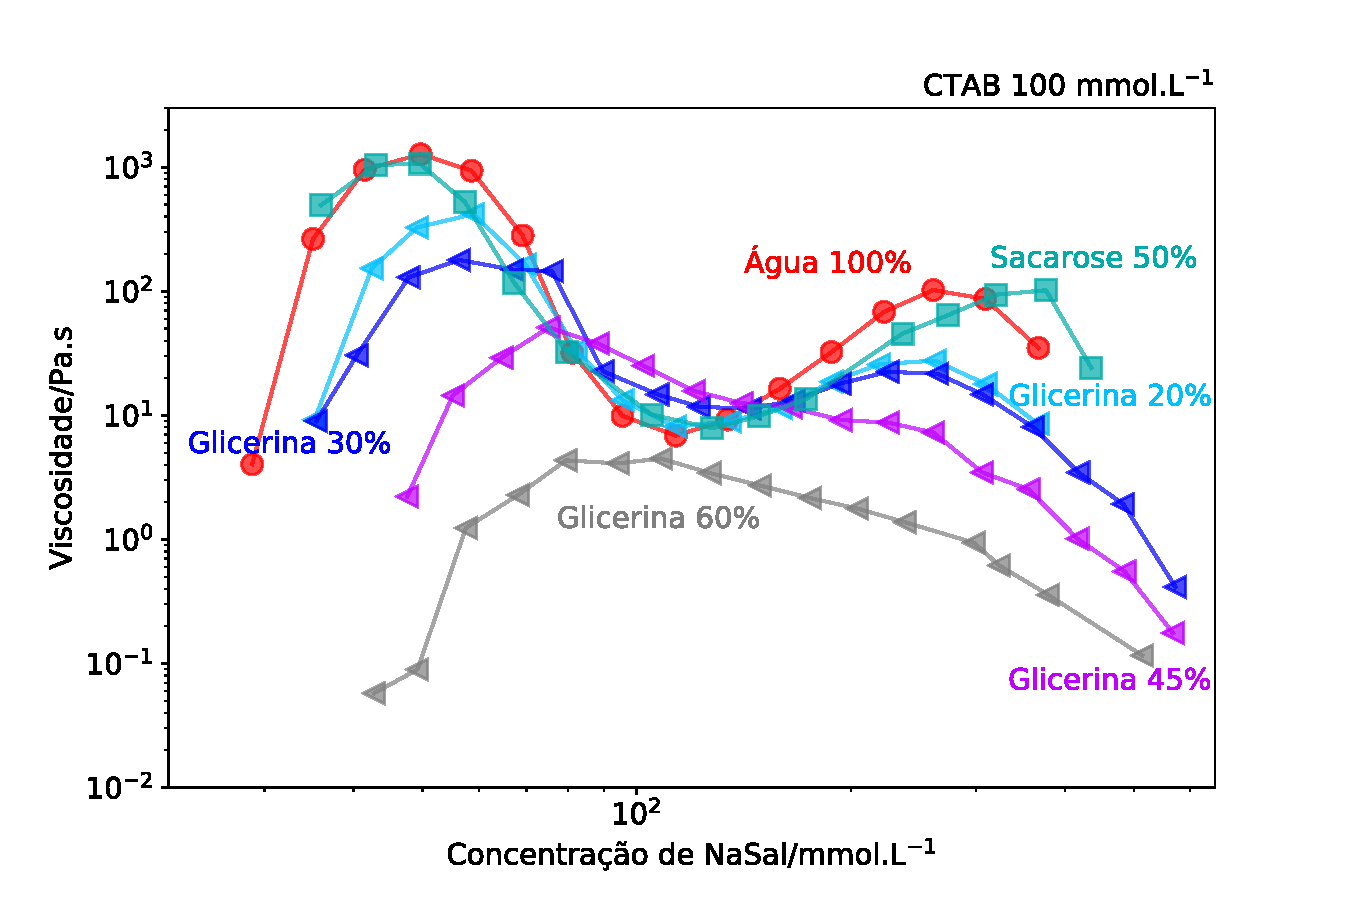
\includegraphics[width=0.7\textwidth]{imagens/reologia/RH_sacarose_glicerina}
				%\caption[Diagrama de viscosidade para glicerina e sacarose]{Viscosidade no repouso \(\eta_0\) em função da concentração de salicilato de sódio (NaSal) em várias concentrações dos aditivos glicerina e sacarose. 60\% de glicerina (V/V) e 50\% de sacarose (m/m) estão no ponto de equivalência do índice de refração. As curvas com 30, 45 e 60 \% de glicerina foram obtidas pela aluna de mestrado Laila Lorenzetti, coautora do trabalho.}
				\caption{Viscosidade no repouso \(\eta_0\) em função da concentração de salicilato de sódio (NaSal) em várias concentrações dos aditivos glicerina e sacarose.
				%	 A concentração de \CTAB{} é de 100 \mM{}.
					60\% de glicerina (V/V) e 50\% de sacarose (m/m) estão no ponto de equivalência do índice de refração. As curvas com 30, 45 e 60 \% de glicerina foram obtidas pela aluna de mestrado Laila Lorenzetti, coautora do trabalho.}
				\label{fig:rh_sacarose_glicerina}
			\end{figure} \index{resultados!sacarose} \index{resultados!glicerina} \index{resultados!\CTAB}
			
			\begin{figure}[htb]
				\centering
				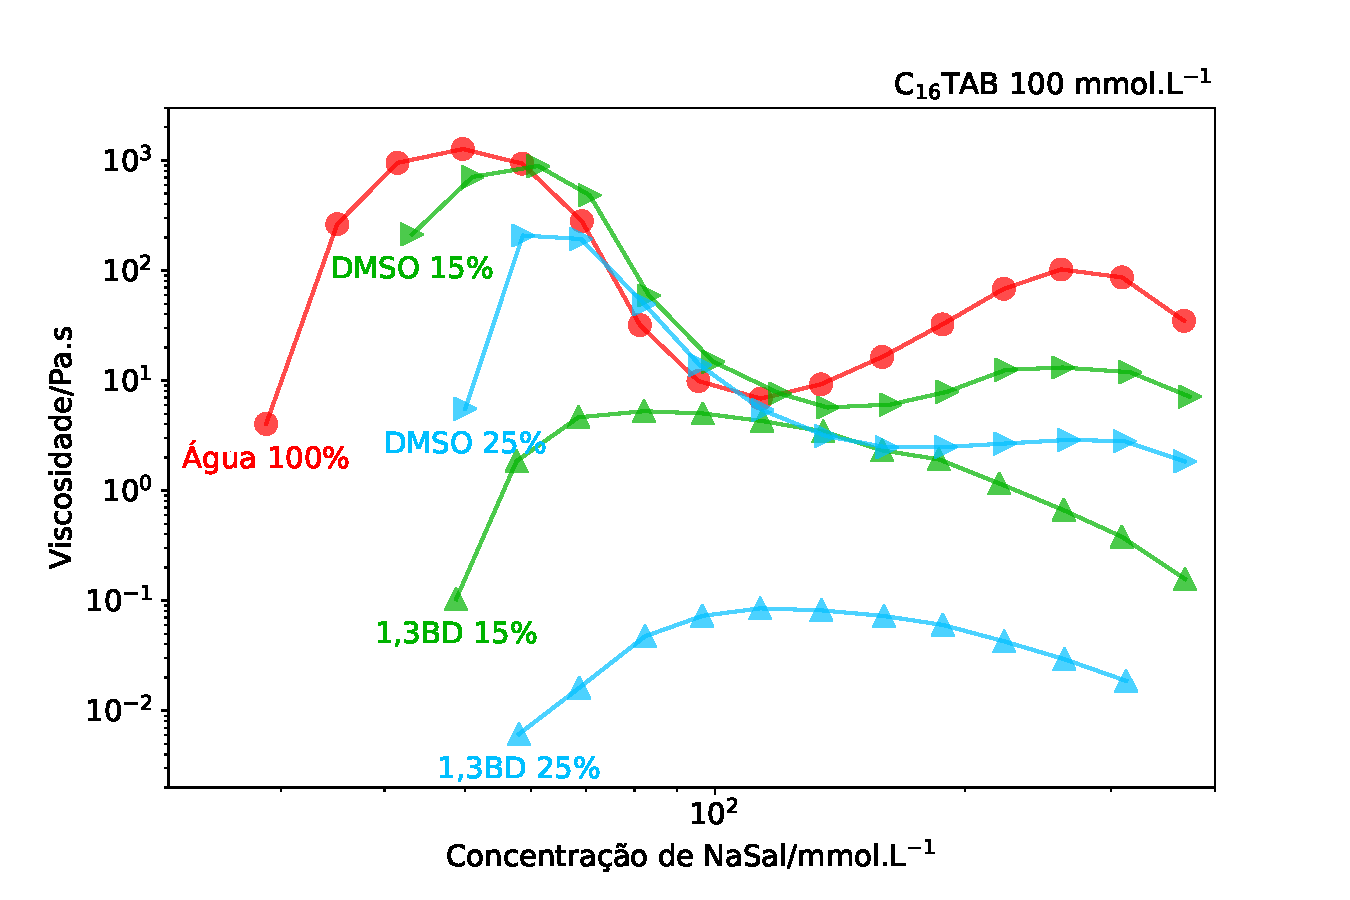
\includegraphics[width=0.7\textwidth]{imagens/reologia/RH_13BD_DMSO}
				%\caption[Diagrama de viscosidade para DMSO e 1,3BD]{Viscosidade no repouso \(\eta_0\) em função da concentração de salicilato de sódio (NaSal) em várias concentrações dos aditivos 1,3-butanodiol (\BD) e dimetilsulfóxido (DMSO). As concentrações de igualdade do índice de refração são 77\% (m/m) e 57\% (m/m), respectivamente}
				\caption{Viscosidade no repouso \(\eta_0\) em função da concentração de salicilato de sódio (NaSal) em várias concentrações dos aditivos 1,3-butanodiol (\BD) e dimetilsulfóxido (DMSO).
					%A concentração de \CTAB{} é de 100 \mM{}.
					As concentrações de igualdade do índice de refração são 77\% (m/m) e 57\% (m/m), respectivamente}
				\label{fig:rh_13bd_dmso}
			\end{figure} \index{resultados!dimetilsulfóxido} \index{resultados!1,3-butanodiol}
			
			\begin{figure}[htb]
				\centering
				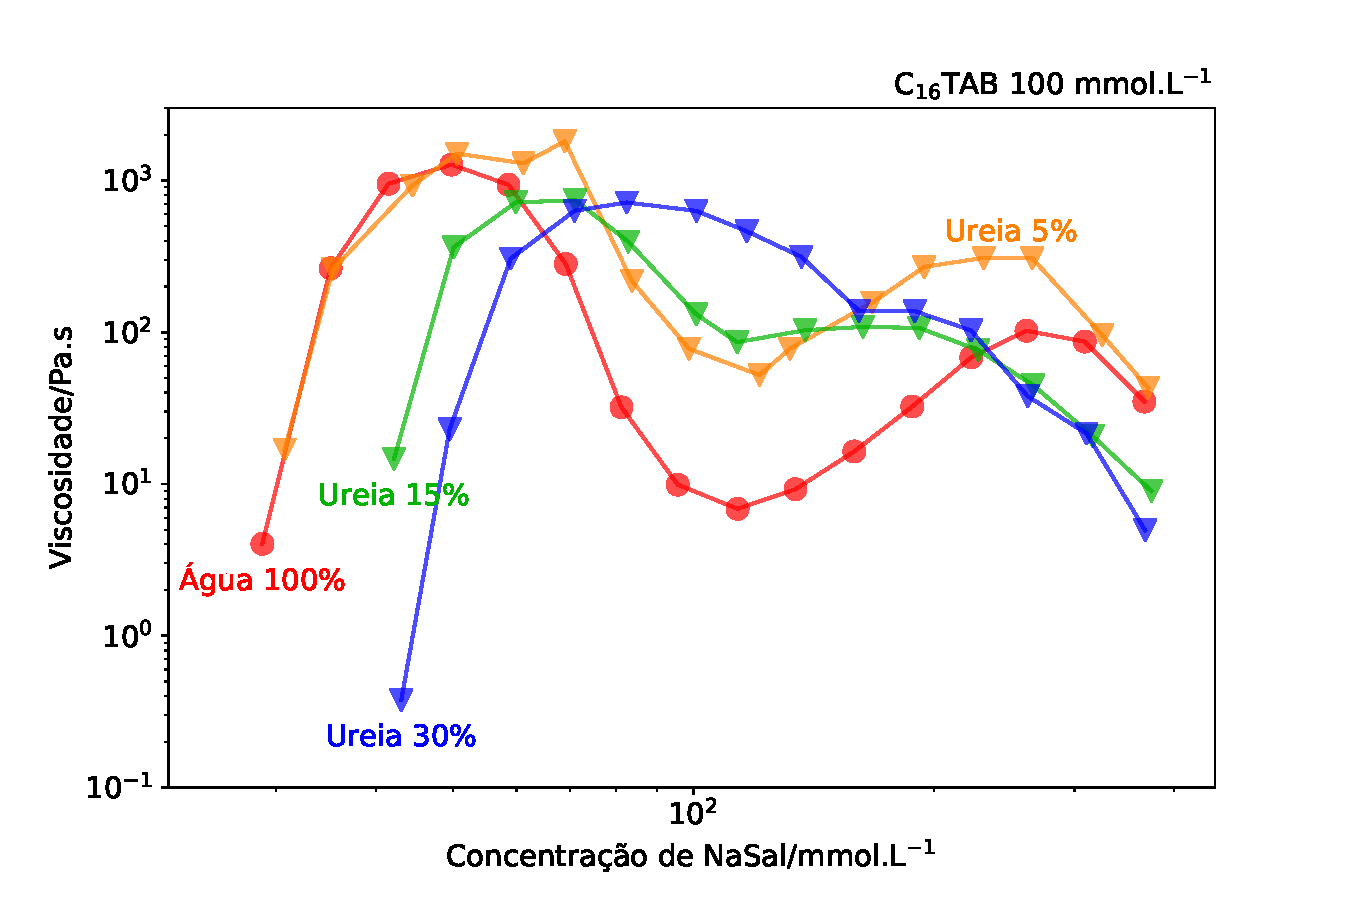
\includegraphics[width=0.7\textwidth]{imagens/reologia/RH_ureia}
				\caption{Viscosidade no repouso \(\eta_0\) em função da concentração de salicilato de sódio (NaSal) em várias concentrações de ureia.
				%	A concentração de \CTAB{} é de 100 \mM{}.
					 A concentração de igualdade de índice de refração é em torno de 55\%.}
				\label{fig:rh_ureia}
			\end{figure} \index{resultados!ureia}
			
			Os dois picos de viscosidade observados em pequenas concentrações de glicerina diminuem, e a região central permanece pouco afetada, como já havia sido observado.\cite{Hoffmann2010} Porém, vemos que a adição de 50\% de sacarose praticamente não afetou a viscosidade das soluções, apesar da igualdade no índice de refração dessas soluções. Isso mostra que considerar somente o índice de refração não permite a previsão do comportamento dessas soluções. O perfil de viscosidade de DMSO e \BD{} foi muito mais afetado pelos aditivos do que era esperado observando-se somente o índice de refração, em especial o 1,3-butanodiol, onde 15\% (m/m) possui o mesmo efeito na viscosidade que 60\% de glicerina. No caso da ureia, a viscosidade na região central aumentou, algo não observado nos outros aditivos, porém o perfil é semelhante a outro já observado em água, com orto-hidróxicinamato e \CTAB{} em pH 9. \cite{Clinckspoor2015}
			
		\FloatBarrier
		
		\section{Efeito dos aditivos na calorimetria de micelas gigantes} \index{resultados!ITC} \index{resultados!\TTAB}
		\label{sec:efeito_aditivos_calorimetria_mg}
			A calorimetria de titulação isotérmica fornece informações sobre o quão favorável é a formação das micelas, através da concentração de formação de micelas gigantes, \cwlm. As Figuras \ref{fig:itc_mg_glicerina}%,
			% \ref{fig:itc_mg_sacarose}, \ref{fig:itc_mg_13bd}, \ref{fig:itc_mg_dmso} e 
			--- \ref{fig:itc_mg_ureia} mostram os perfis de formação de micelas gigantes para glicerina, sacarose, 1,3-butanodiol, dimetilsulfóxido e ureia, respectivamente. 
		
			\begin{figure}[h]
				\centering
				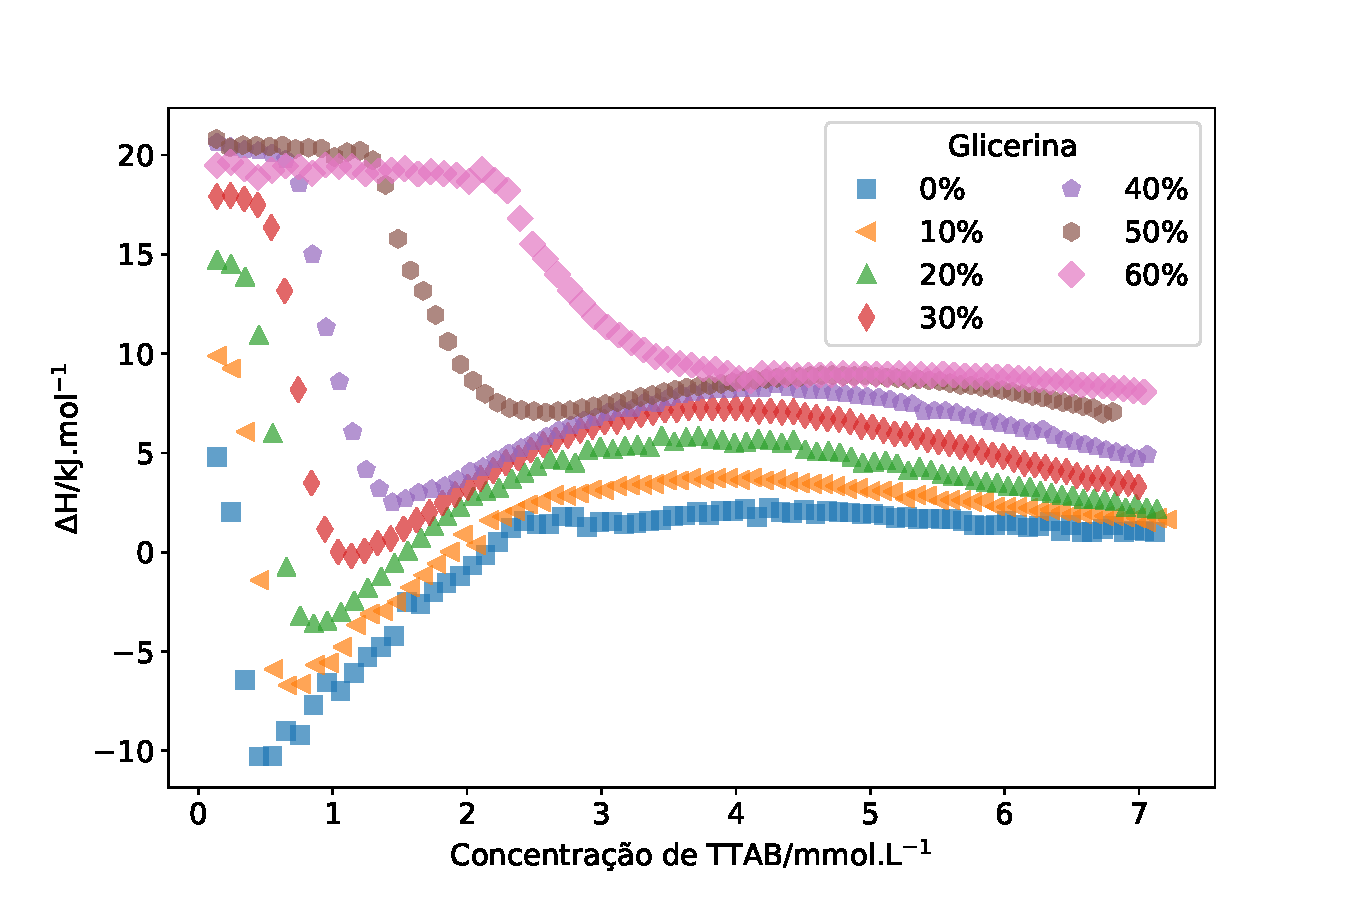
\includegraphics[width=0.7\textwidth]{imagens/itc/ITC_MG_glic}
				\caption{Efeito da concentração de glicerina nas curvas de titulação de formação de micelas gigantes. A concentração de salicilato de sódio na cela de amostra é de 1,5 \mM. A concentração do aditivo está em \% (V/V).}
				\label{fig:itc_mg_glicerina}
			\end{figure}  \index{resultados!glicerina}
			
			\begin{figure}[h]
				\centering
				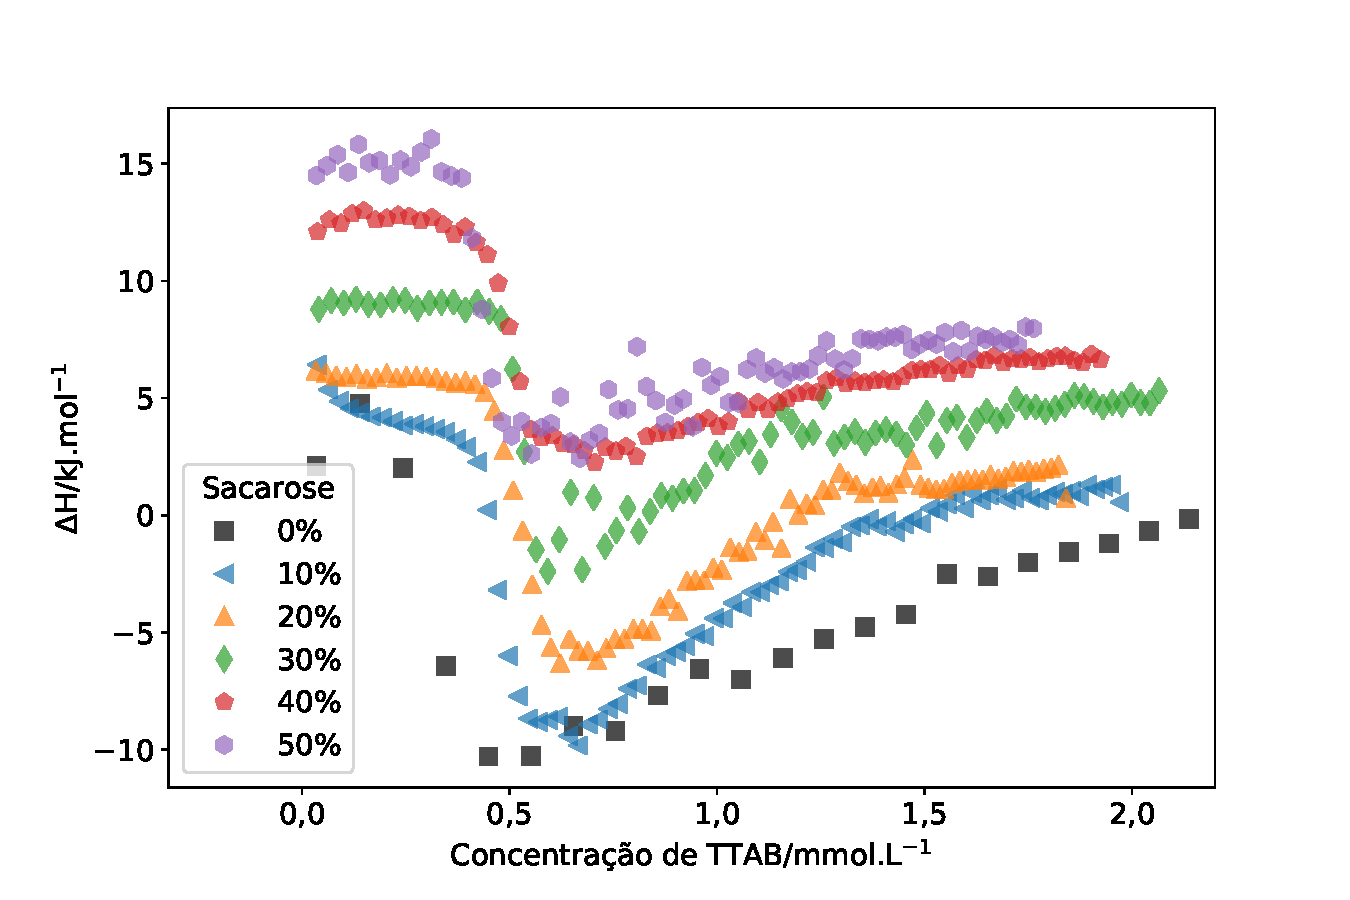
\includegraphics[width=0.7\textwidth]{imagens/itc/ITC_MG_sac}
				\caption{Efeito da concentração de sacarose nas curvas de titulação de formação de micelas gigantes. A concentração de salicilato de sódio na cela de amostra é de 1,5 \mM. A concentração do aditivo está em \% (m/m).}
				\label{fig:itc_mg_sacarose}
			\end{figure} \index{resultados!sacarose}
			
						
			\begin{figure}[h]
				\centering
				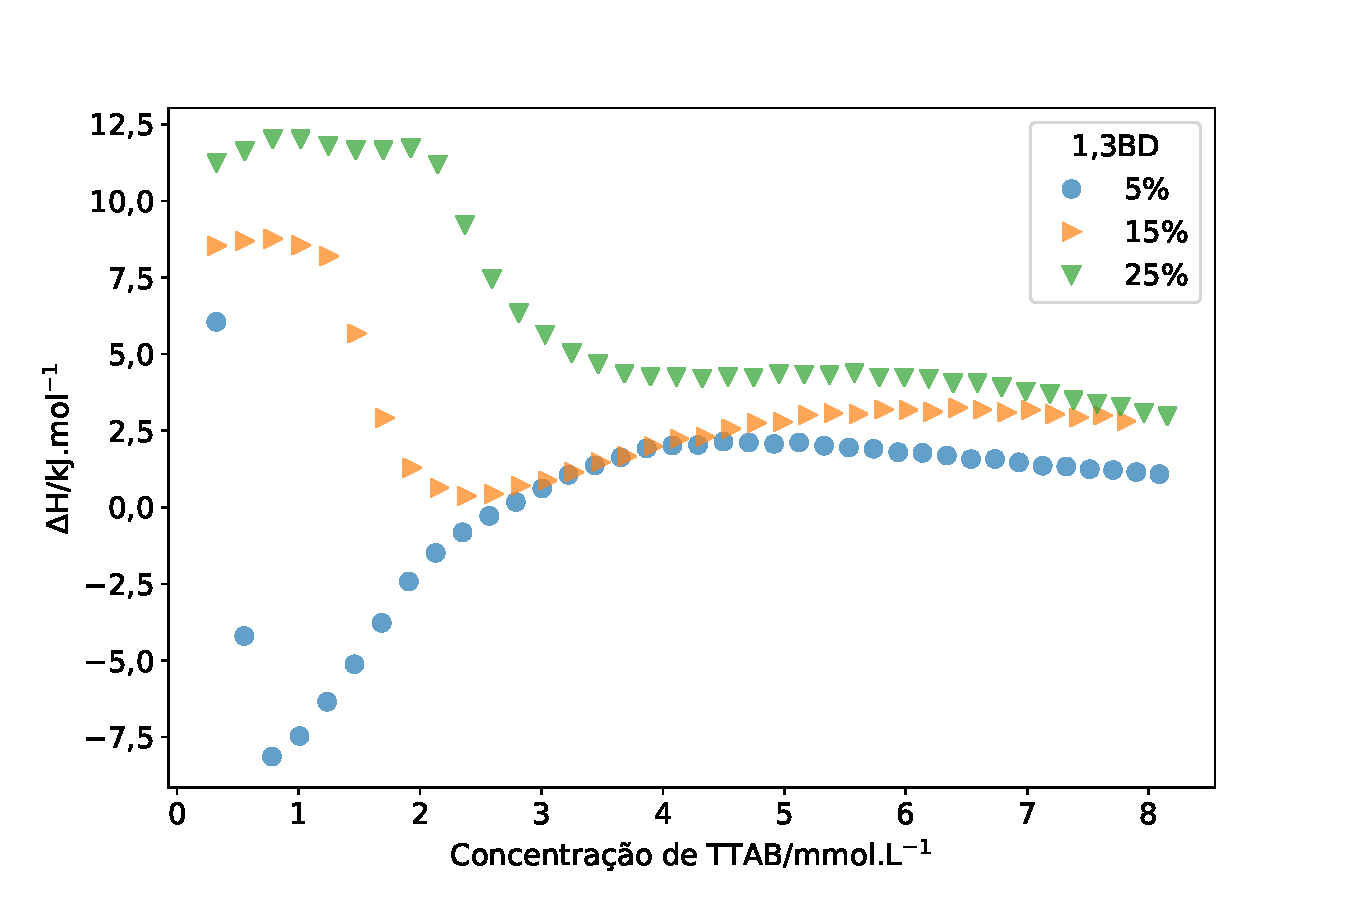
\includegraphics[width=0.7\textwidth]{imagens/itc/ITC_MG_13BD}
				\caption{Efeito da concentração de 1,3-butanodiol nas curvas de titulação de formação de micelas gigantes. A concentração de salicilato de sódio na cela de amostra é de 1,5 \mM. A concentração do aditivo está em \% (m/m).}
				\label{fig:itc_mg_13bd}
			\end{figure} \index{resultados!1,3-butanodiol}
			
			\begin{figure}[h]
				\centering
				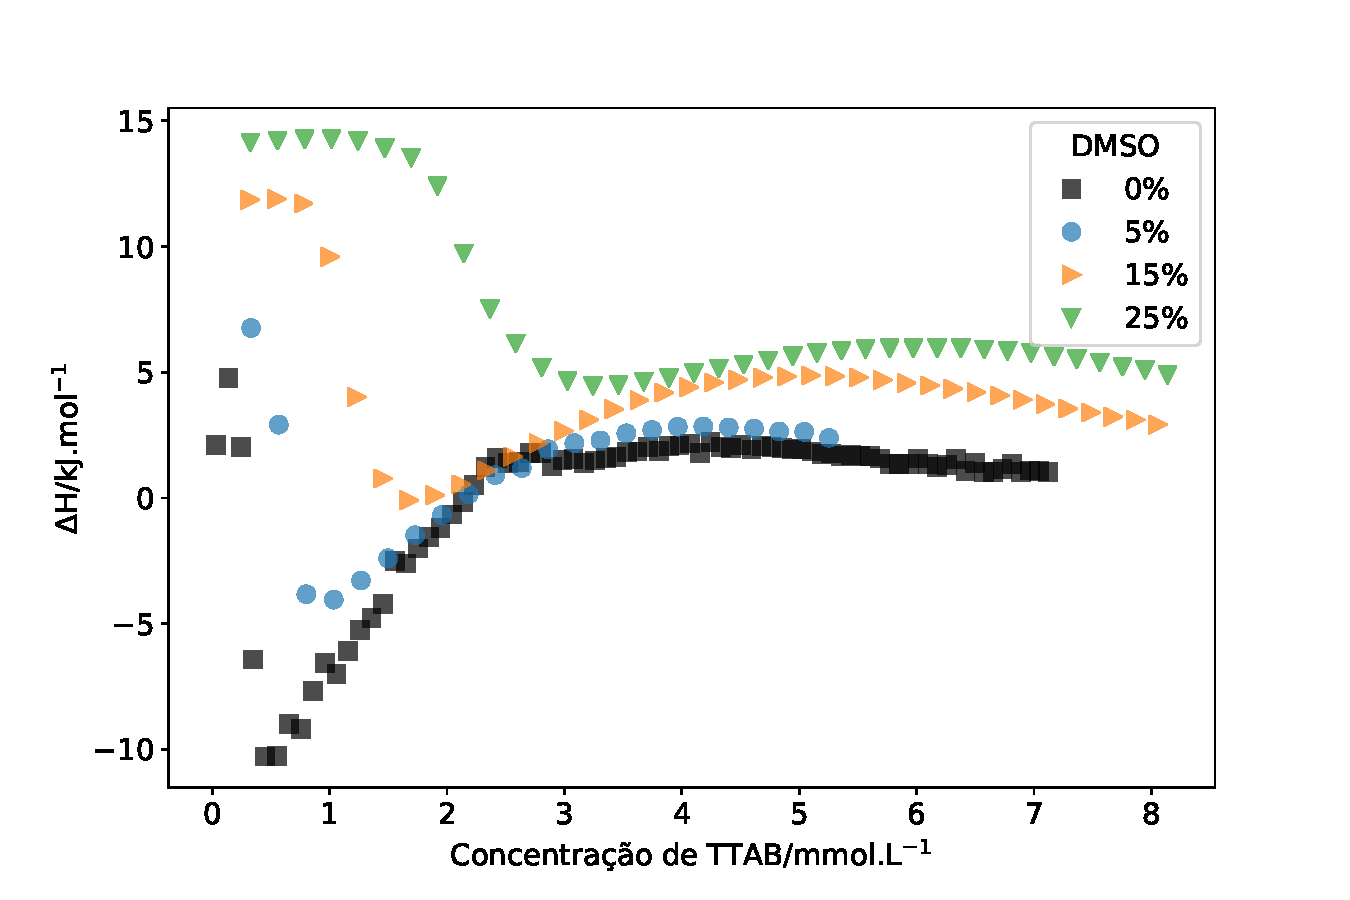
\includegraphics[width=0.7\textwidth]{imagens/itc/ITC_MG_dmso}
				\caption{Efeito da concentração de dimetilsulfóxido nas curvas de titulação de formação de micelas gigantes. A concentração de salicilato de sódio na cela de amostra é de 1,5 \mM. A concentração do aditivo está em \% (m/m).}
				\label{fig:itc_mg_dmso} \index{resultados!dimetilsulfóxido}
			\end{figure}

			\begin{figure}[h]
				\centering
				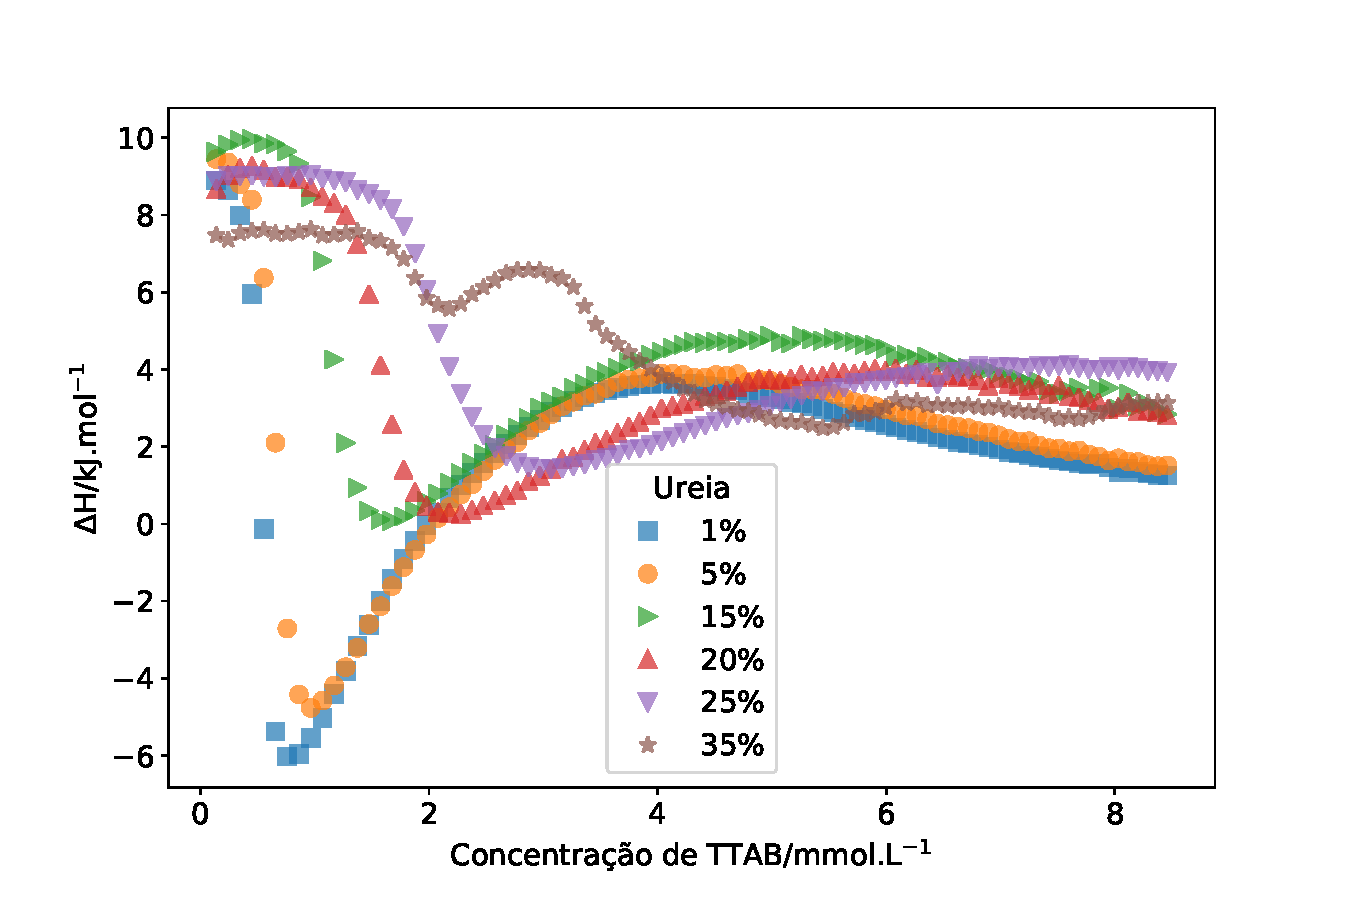
\includegraphics[width=0.7\textwidth]{imagens/itc/ITC_MG_ur}
				\caption{Efeito da concentração de ureia nas curvas de titulação de formação de micelas gigantes. A concentração de salicilato de sódio na cela de amostra é de 1,5 \mM. A concentração do aditivo está em \% (m/m).}
				\label{fig:itc_mg_ureia}
			\end{figure} \index{resultados!ureia}
			
			
			As diferenças entre glicerina e sacarose, novamente, se evidenciaram. Da mesma maneira que na reologia, a presença de sacarose não afetou a formação de micelas gigantes. Já a glicerina teve um efeito deletério na autoassociação, aumentando significativamente a concentração necessária para o crescimento. \BD{} e DMSO não se mostraram muito diferentes, apesar dos perfis reológicos serem bastante distintos, algo não totalmente inesperado, já que ambas as técnicas observam fenômenos diferentes. Isso indica que o \BD{} não leva à uma diminuição na estabilidade micelar, o que poderia levar à uma diminuição na quantidade de micelas, que poderia diminuir a viscosidade dos sistemas. Logo, o \BD{} possui outros mecanismos que afetam as micelas.

			O comportamento da ureia seguiu o esperado, de acordo com a literatura\cite{Souza2012, Bruning1961}, com um aumento de \cwlm{}. É interessante notar que o \DHwlm{} diminui com o aumento da concentração de ureia, o que sugere uma diminuição na adsorção de salicilato nas micelas. Em 35\% de ureia observa-se um perfil bastante diferente dos outros, porém nessa situação, ocorre a formação de um precipitado, cuja natureza será discutida na \autoref{sec:cap_efeito_ureia}.
			
			Uma maneira de se resumir as curvas calorimétricas é utilizando somente a concentração de formação de micelas gigantes (\cwlm) e a entalpia de micelização (\DHwlm). Dessa forma, podemos comparar o efeito da concentração dos aditivos nas curvas mais facilmente, como mostra a \autoref{fig:cwlm_dhwlm_por_conc}. Esse tipo de figura, utilizando outras propriedades na abcissa, será utilizado para realizar novas comparações futuramente.
			
%			\begin{figure}[h]
%				\begin{subfigure}[t]{0.5\textwidth}
%					\centering
%					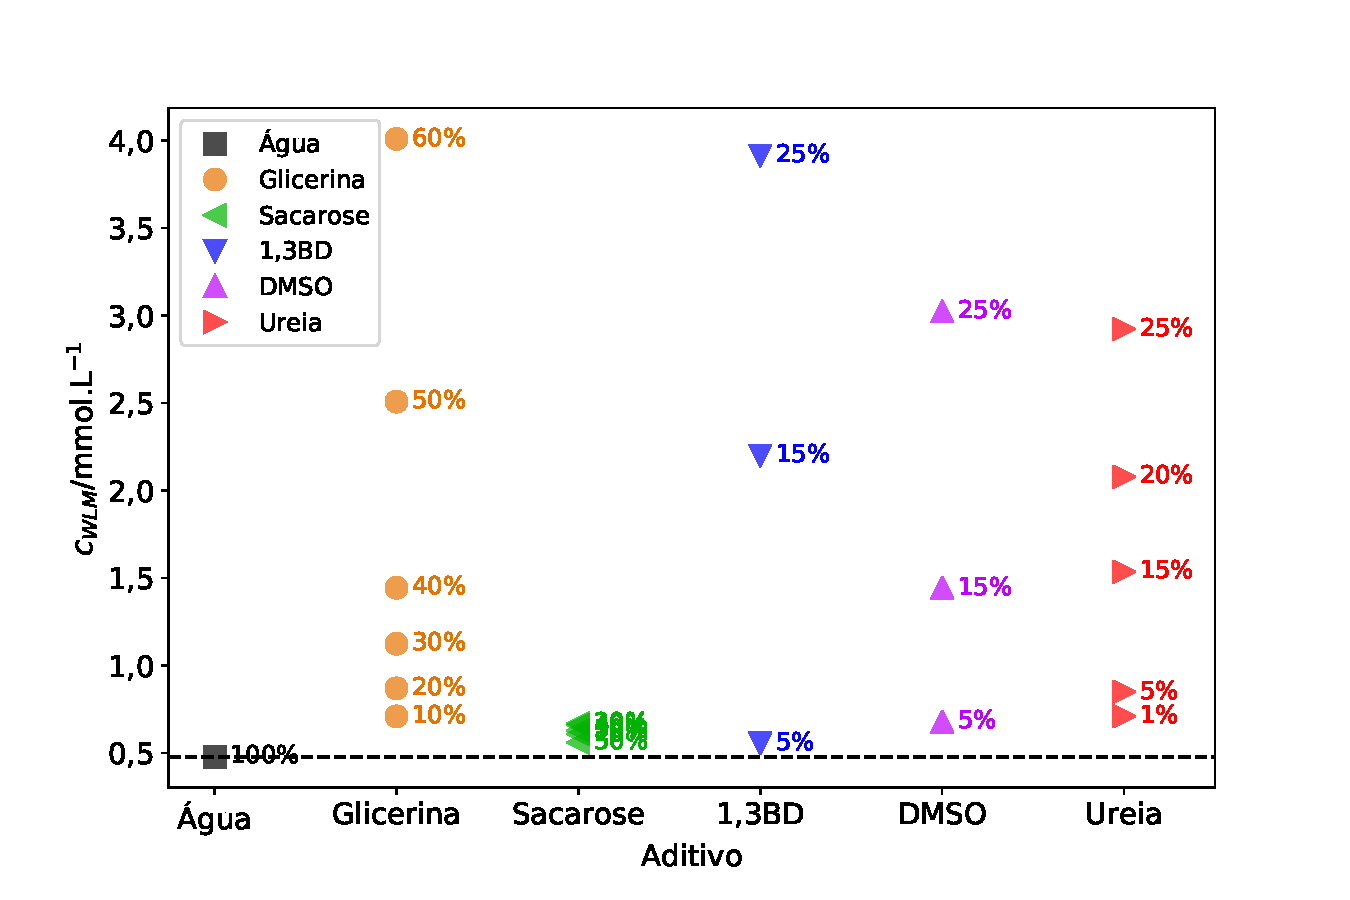
\includegraphics[width=\textwidth]{imagens/itc/Cwlm_por_Aditivo}
%					\caption{\cwlm{}}
%					\label{fig:cwlm_por_aditivo}
%				\end{subfigure}%
%				\begin{subfigure}[t]{0.5\textwidth}
%					\centering
%					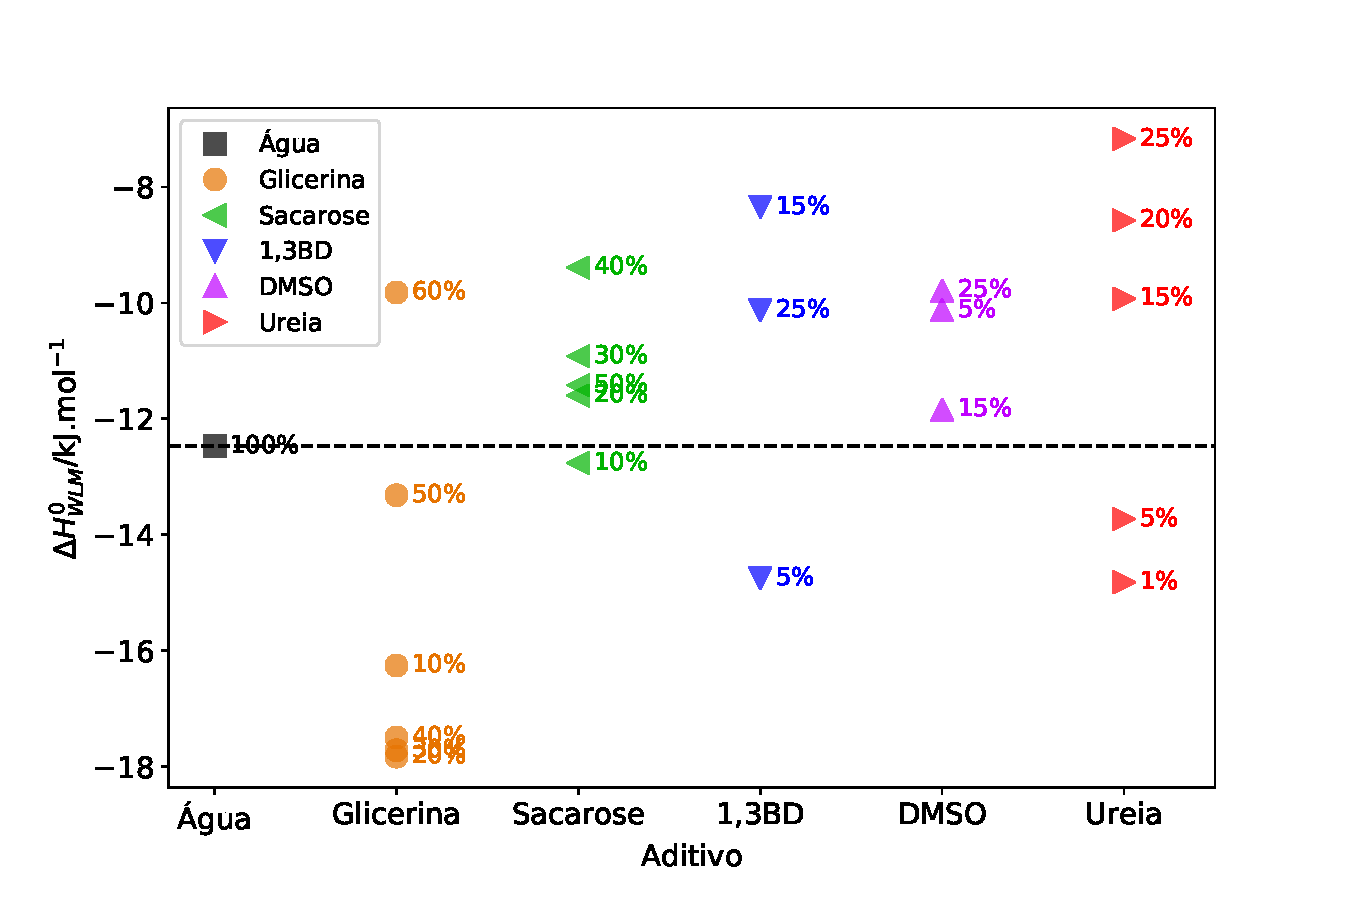
\includegraphics[width=\textwidth]{imagens/itc/DHwlm_por_Aditivo}
%					\caption{\DHwlm{}}
%					\label{fig:dhwlm_por_aditivo}
%				\end{subfigure}
%				\caption{\cwlm{} e \DHwlm{} em função dos aditivos e de sua concentração}
%				\label{fig:cwlm_dhwlm_por_aditivo} % todo: se tiver tempo, alterar o Delta H 0 para Delta H \circ
%			\end{figure} 
		
			\begin{figure}[h]
				\begin{subfigure}[t]{0.5\textwidth}
					\centering
					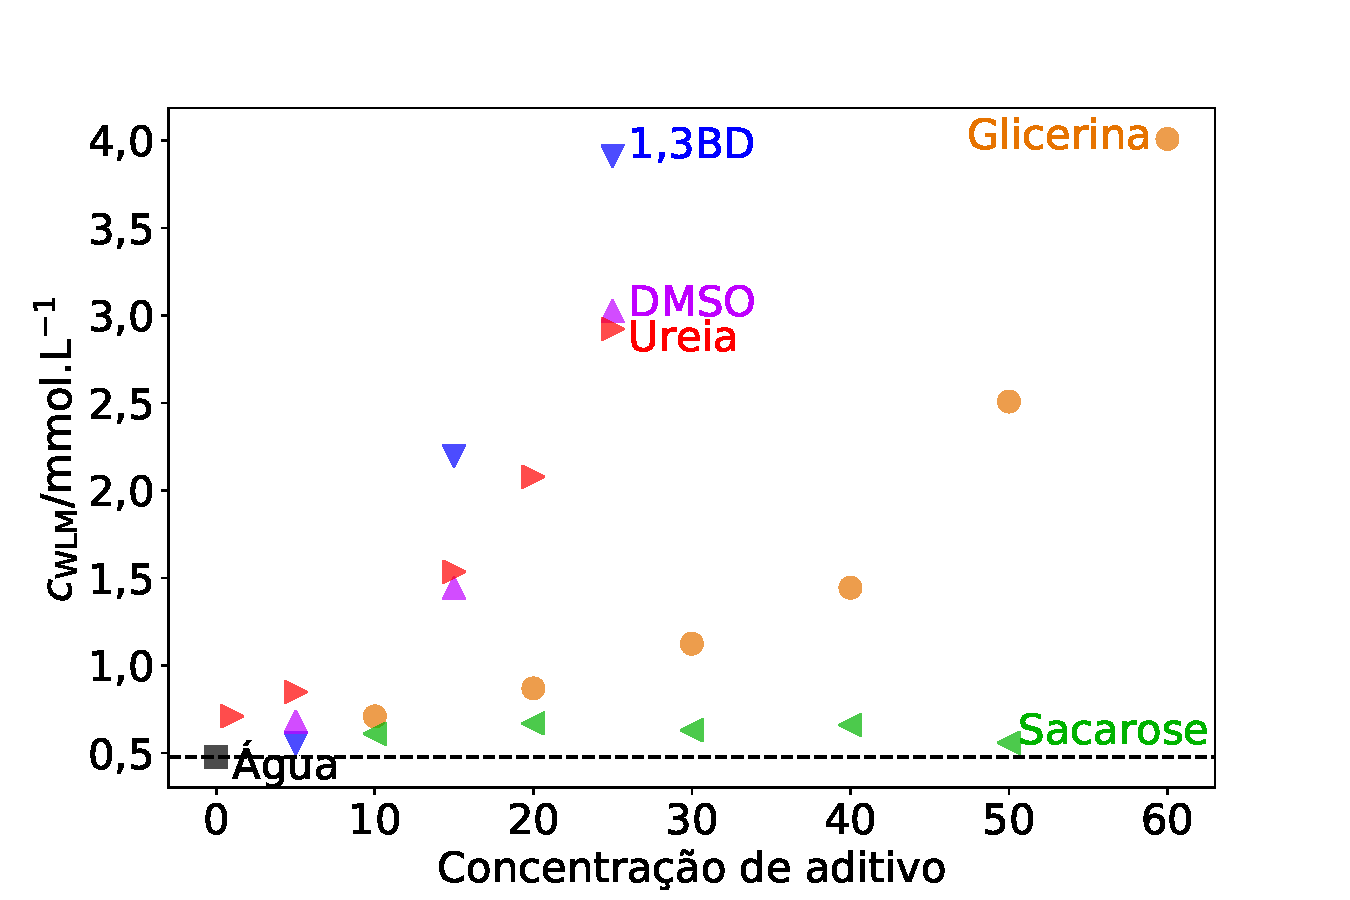
\includegraphics[width=\textwidth]{imagens/itc/Cwlm_por_conc}
					\caption{\cwlm}
					\label{fig:cwlm_por_conc}
				\end{subfigure} %
				\begin{subfigure}[t]{0.5\textwidth}
					\centering
					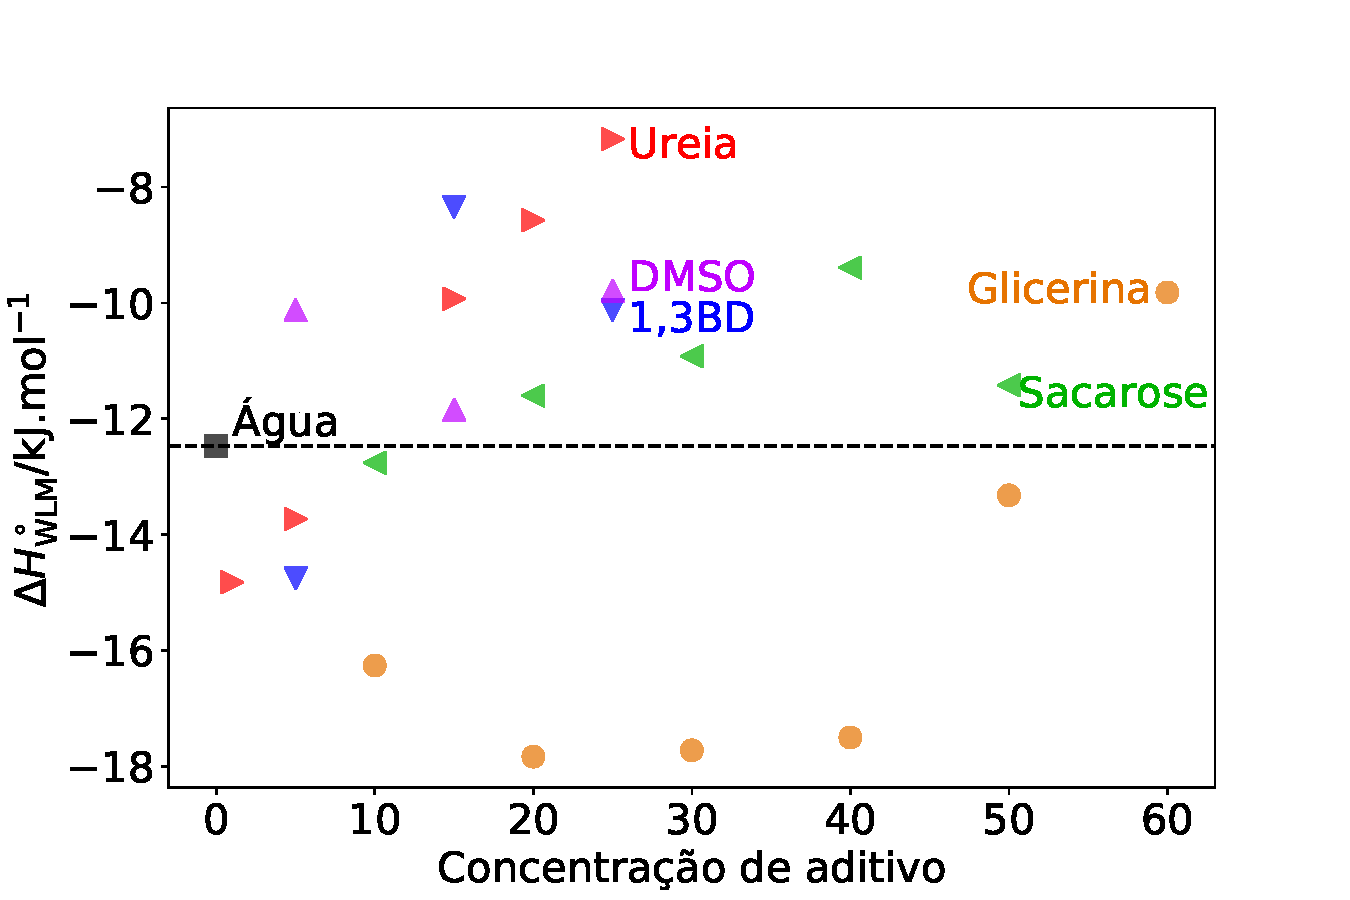
\includegraphics[width=\textwidth]{imagens/itc/DHwlm_por_conc}
					\caption{\DHwlm}
					\label{fig:dhwlm_por_conc}
				\end{subfigure}
				
				\caption{\cwlm{} e \DHwlm{}, obtidas das Figuras \ref{fig:itc_mg_glicerina}---\ref{fig:itc_mg_ureia} em função da concentração de aditivo para titulações de \TTAB{} em NaSal 1,5 \mM. A concentração do aditivo está em \% (m/m).}
				\label{fig:cwlm_dhwlm_por_conc}
			\end{figure}

		Vemos então claramente que os efeitos dos aditivos na \cwlm{} são relativamente bem comportados, com tendências claras para cada aditivo. Já para a \DHwlm, os tendência aparenta ser um pouco caótica, com valores que aumentam e diminuem, como no caso da glicerina.

		\FloatBarrier
		
		\section{Efeito dos aditivos na calorimetria de micelização} \index{resultados!ITC} \index{resultados!\TTAB}
		\label{sec:efeito_aditivos_calorimetria_me}
		A calorimetria de formação de micelas gigantes possui uma complexidade maior devido à presença do salicilato. Para facilitar a interpretação, foram obtidas informações da formação de micelas esféricas, titulando-se \TTAB{} em água. As Figuras \ref{fig:itc_glicerina}, \ref{fig:itc_sacarose}, \ref{fig:itc_13bd}, \ref{fig:itc_dmso} e \ref{fig:itc_ureia} mostram as curvas de titulação para glicerina, sacarose, 1,3-butanodiol, dimetilsulfóxido e ureia, respectivamente.
					
%			\begin{figure}[h]
%				\centering
%				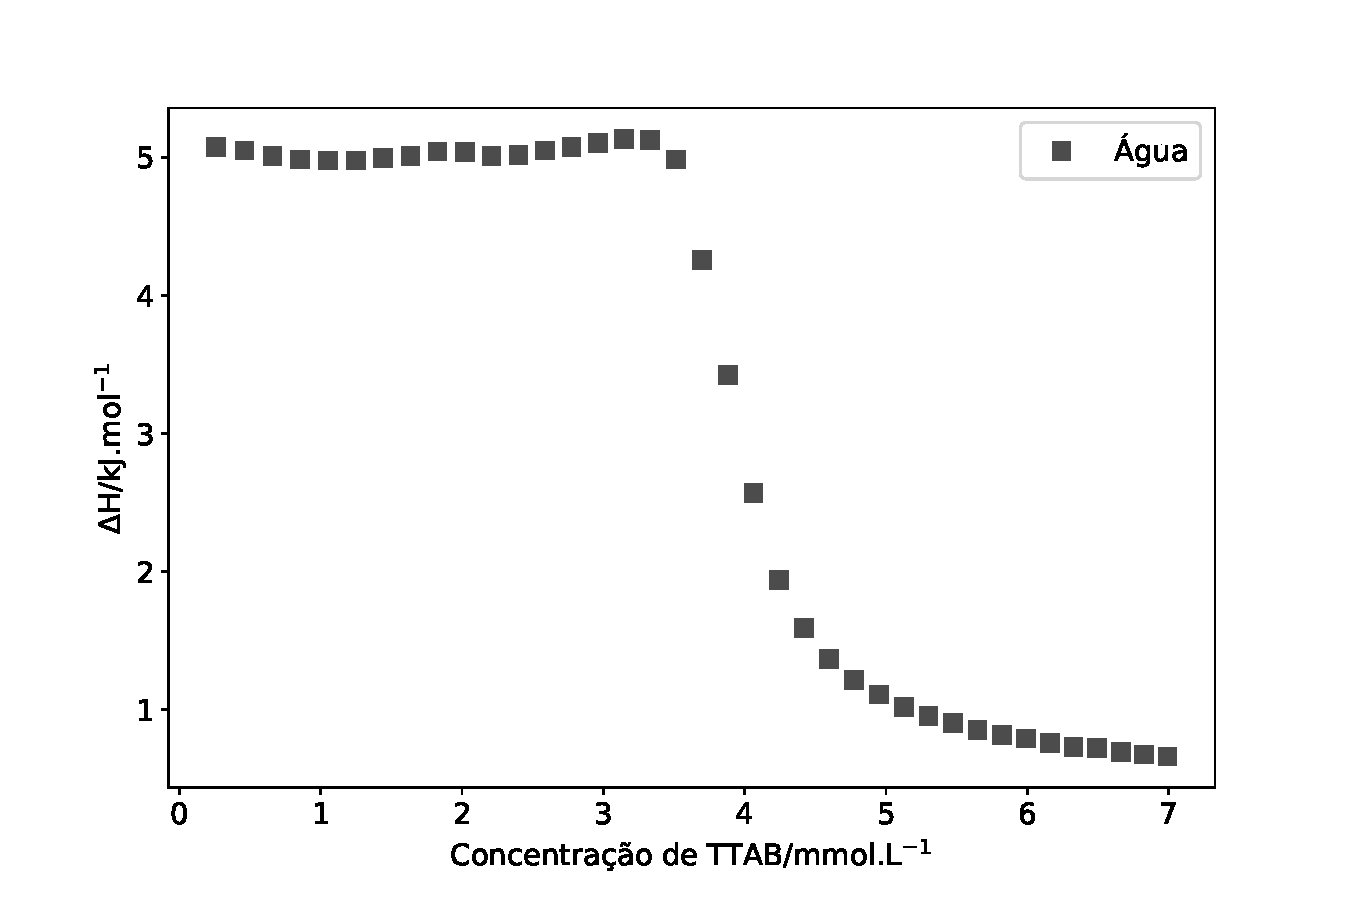
\includegraphics[width=0.7\textwidth]{imagens/itc/ITC_agua}
%				\caption{Titulação de \TTAB em água}
%				\label{fig:itc_agua}
%			\end{figure}
			
			\begin{figure}[h]
				\centering
				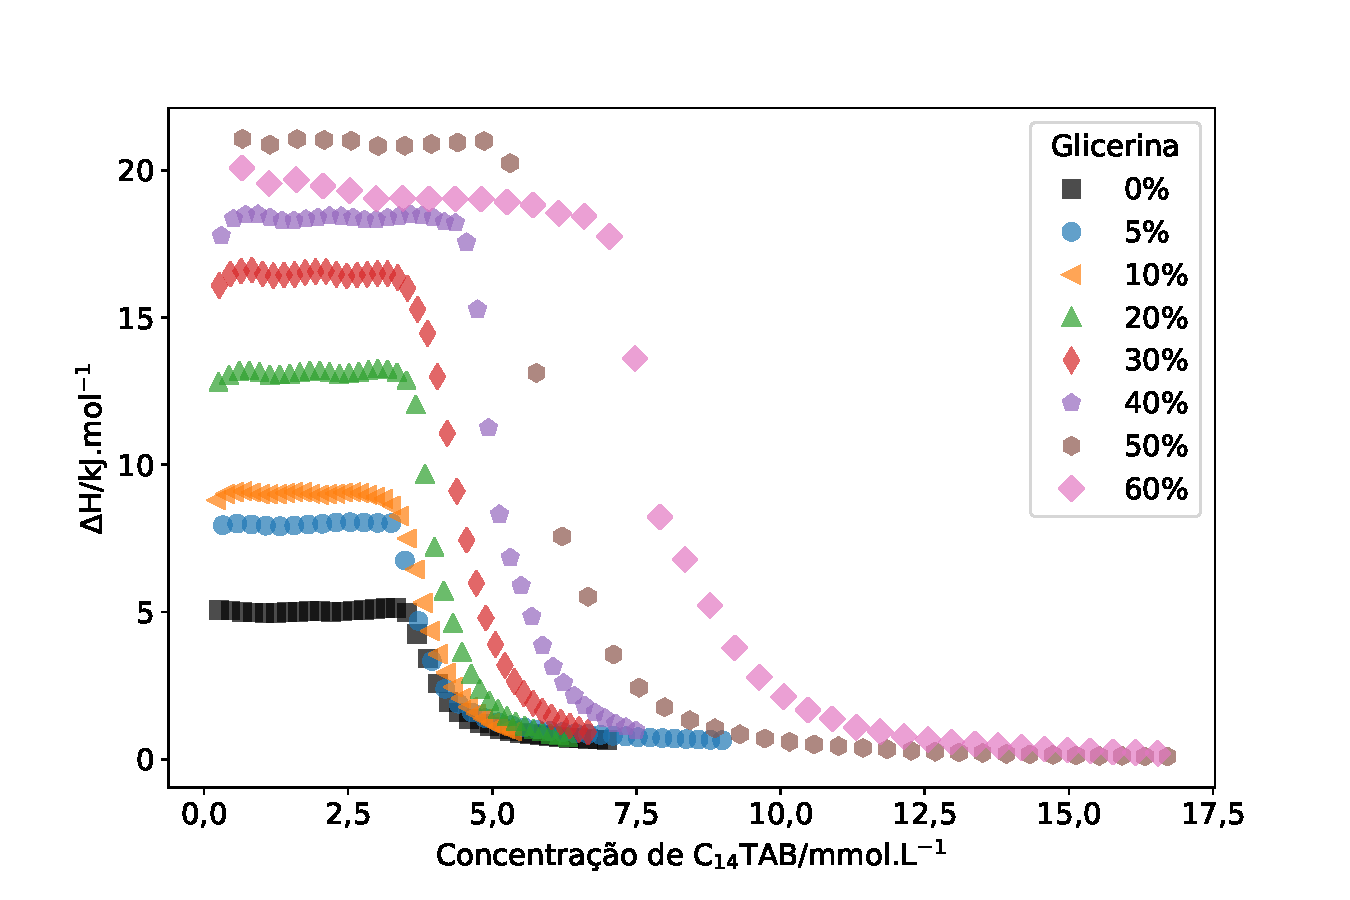
\includegraphics[width=0.7\textwidth]{imagens/itc/ITC_glic}
				\caption{Efeito da glicerina na titulação de \TTAB.}
				\label{fig:itc_glicerina}
			\end{figure} \index{resultados!glicerina}
		
			\begin{figure}[h]
				\centering
				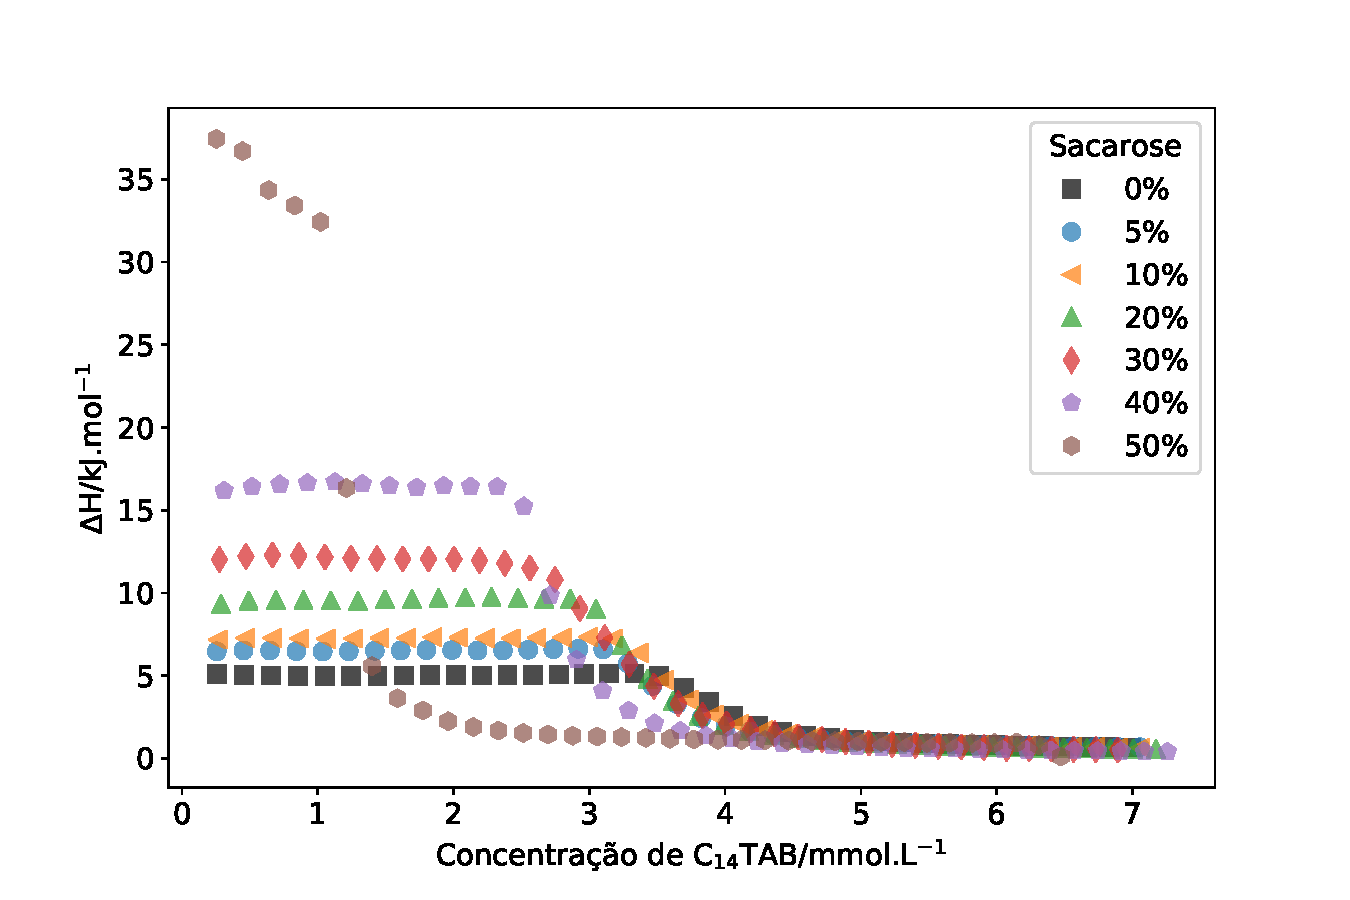
\includegraphics[width=0.7\textwidth]{imagens/itc/ITC_sac}
				\caption{Efeito de sacarose na titulação de \TTAB}
				\label{fig:itc_sacarose}
			\end{figure} \index{resultados!sacarose}
			
			O efeito da glicerina na formação de micelas é semelhante ao efeito em micelas gigantes, exceto pelo aumento do \DHmic{}, na questão da tendência de aumento das concentrações críticas.\cite{Moya2007a} Mais interessante, porém, é que sacarose levou à uma diminuição da \cmc{}. Isso já foi observado para SDS\cite{Bakshi1993a, Chauhan2014}, \CTAB\cite{Banipal2016a} e Brij 35\cite{Sharma1989}. A literatura sugere que a sacarose pode estruturar a água, portanto aumentando a penalidade entrópica e diminuindo a \cmc,\cite{Chauhan2014, Banipal2016a, Sharma1989}, assim como pode interagir com a superfície micelar, diminuindo a repulsão entre as cabeças, estabilizando as micelas.\cite{Bakshi1993a, Chauhan2014, Banipal2016a}. Porém, nas micelas gigantes, o grupo carboxilato do salicilato se encontra nessa mesma região, então há uma competição entre hidroxilas e carboxilatos. Como o carboxilato é carregado, interage mais fortemente com as micelas e impede que a sacarose exerça sua influência estabilizadora, logo não afeta as micelas. O efeito do aumento do índice de refração pode ter sido contrabalanceado pela estruturação do solvente, neste caso.
			
			\begin{figure}[h]
				\centering
				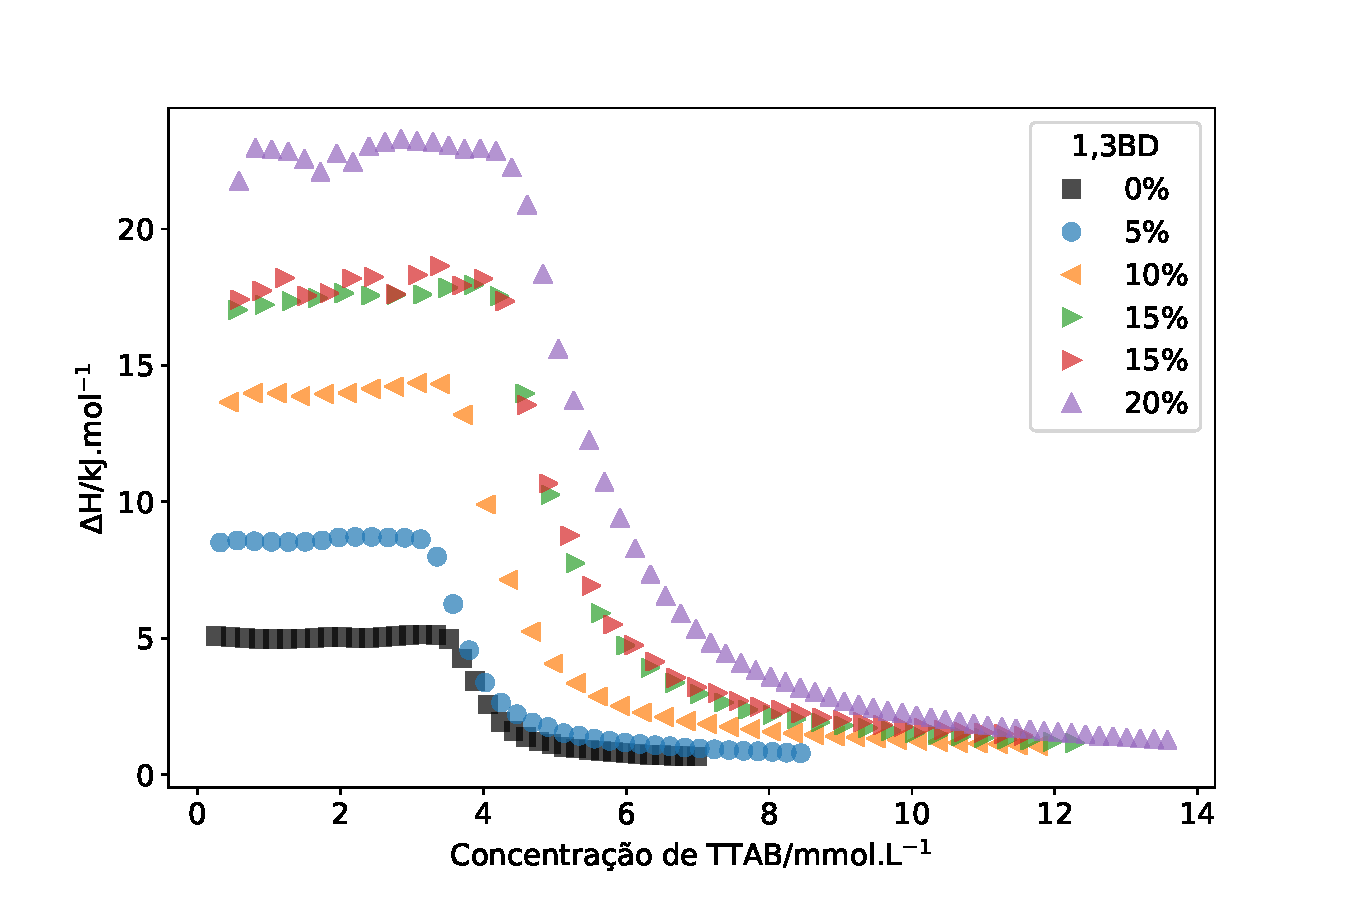
\includegraphics[width=0.7\textwidth]{imagens/itc/ITC_13BD}
				\caption{Efeito de 1,3-butanodiol na titulação de \TTAB}
				\label{fig:itc_13bd}
			\end{figure}  \index{resultados!1,3-butanodiol}
		
			\begin{figure}[h]
				\centering
				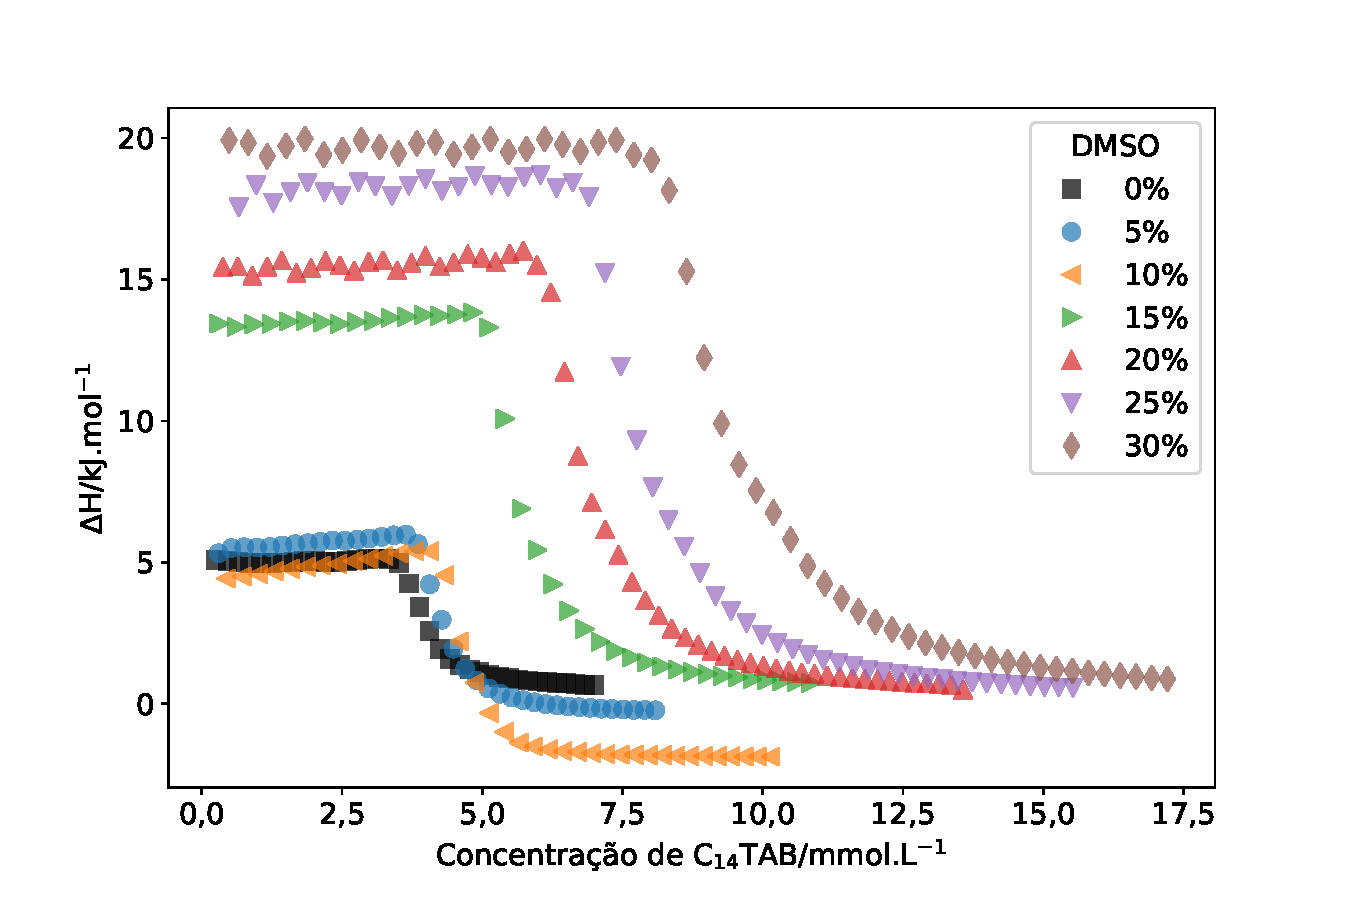
\includegraphics[width=0.7\textwidth]{imagens/itc/ITC_dmso}
				\caption{Efeito de dimetilsulfóxido na titulação de \TTAB.}
				\label{fig:itc_dmso}
			\end{figure} \index{resultados!dimetilsulfóxido}
			
			\begin{figure}[h]
				\centering
				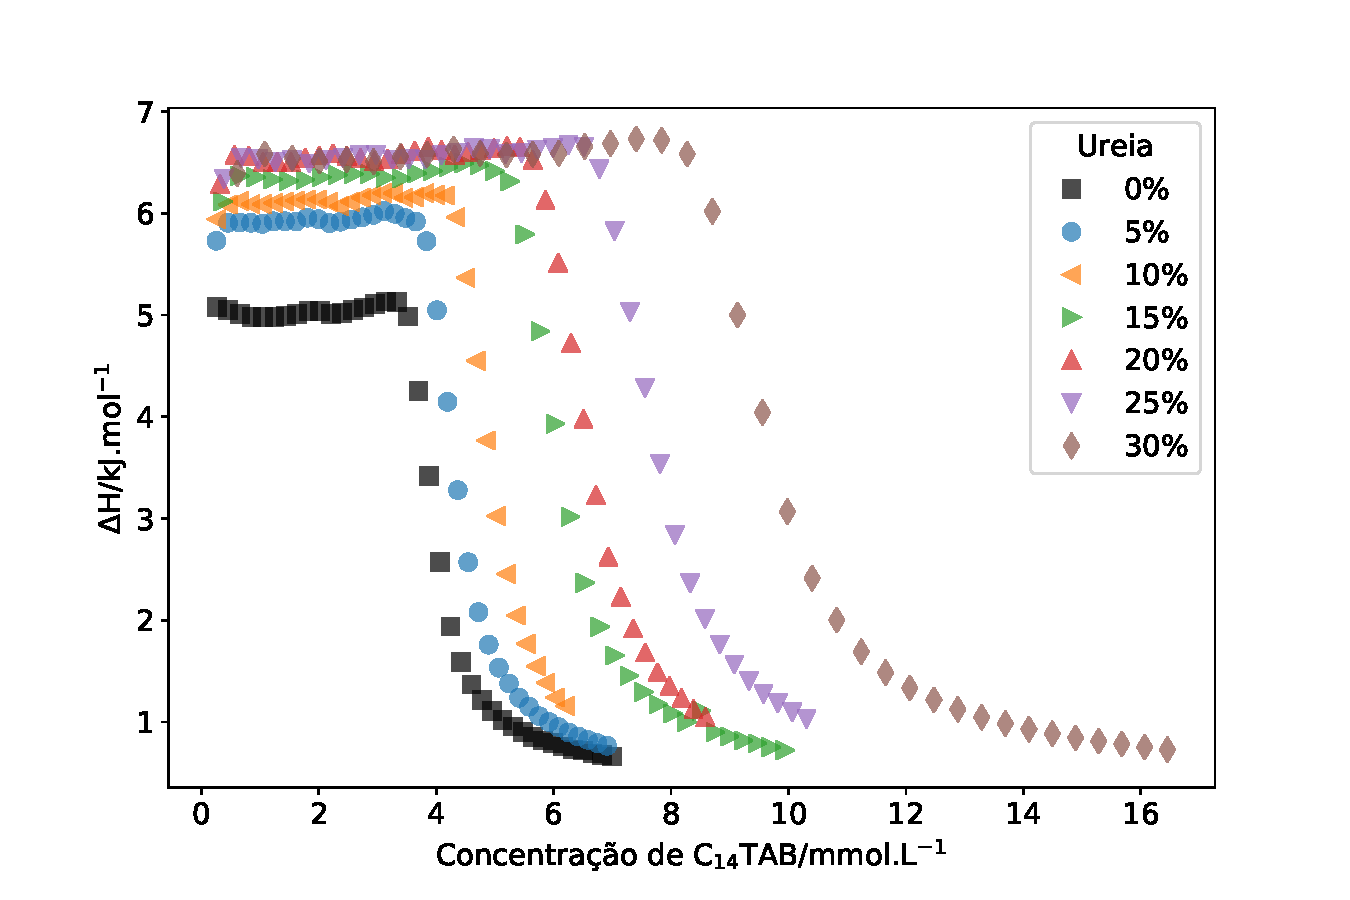
\includegraphics[width=0.7\textwidth]{imagens/itc/ITC_ur}
				\caption{Efeito de ureia na titulação de \TTAB.}
				\label{fig:itc_ureia}
			\end{figure} \index{resultados!ureia}
		
		Novamente, o \BD{} e DMSO mostraram possuir comportamentos semelhantes entre si, portanto o mecanismo que influencia ambas as micelas gigantes quanto esféricas deve ser semelhante. O aumento na \cmc{} já foi observado anteriormente, tanto para o DMSO\cite{Bakshi1993a} quando para \BD.\cite{Abdel-Rahem2012}. A ureia influencia aumentando a \cmc{}, como esperado,\cite{Dias2002} porém não afeta muito o \DHmic{}. Logo, como não há \Sal{} para ser dessorvido das micelas, não ocorrem grandes variações de \DHmic.
		
		\FloatBarrier
		
		Da mesma maneira que anteriormente, essas informações foram resumidas na \autoref{fig:cmc_dh_por_conc}, onde a \cmc{} e o \DHmic{} foram colocados em função da concentração de aditivo.
		
%		\begin{figure}[h]
%			\begin{subfigure}[t]{0.5\textwidth}
%				\centering
%				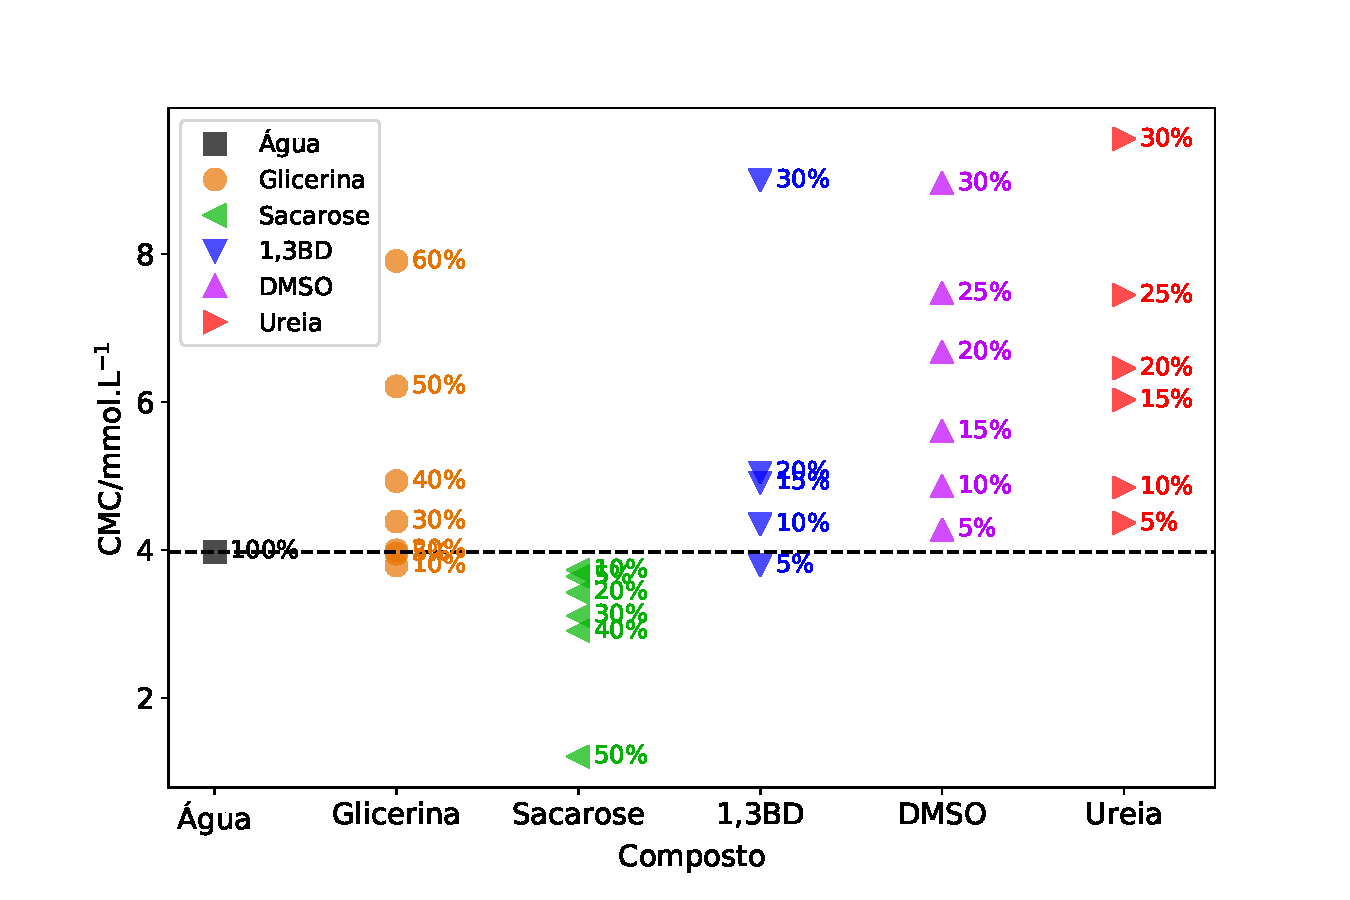
\includegraphics[width=\textwidth]{imagens/itc/CMC_por_composto}
%				\caption{\cmc}
%				\label{fig:cmc_por_composto}
%			\end{subfigure} %
%			\begin{subfigure}[t]{0.5\textwidth}
%				\centering
%				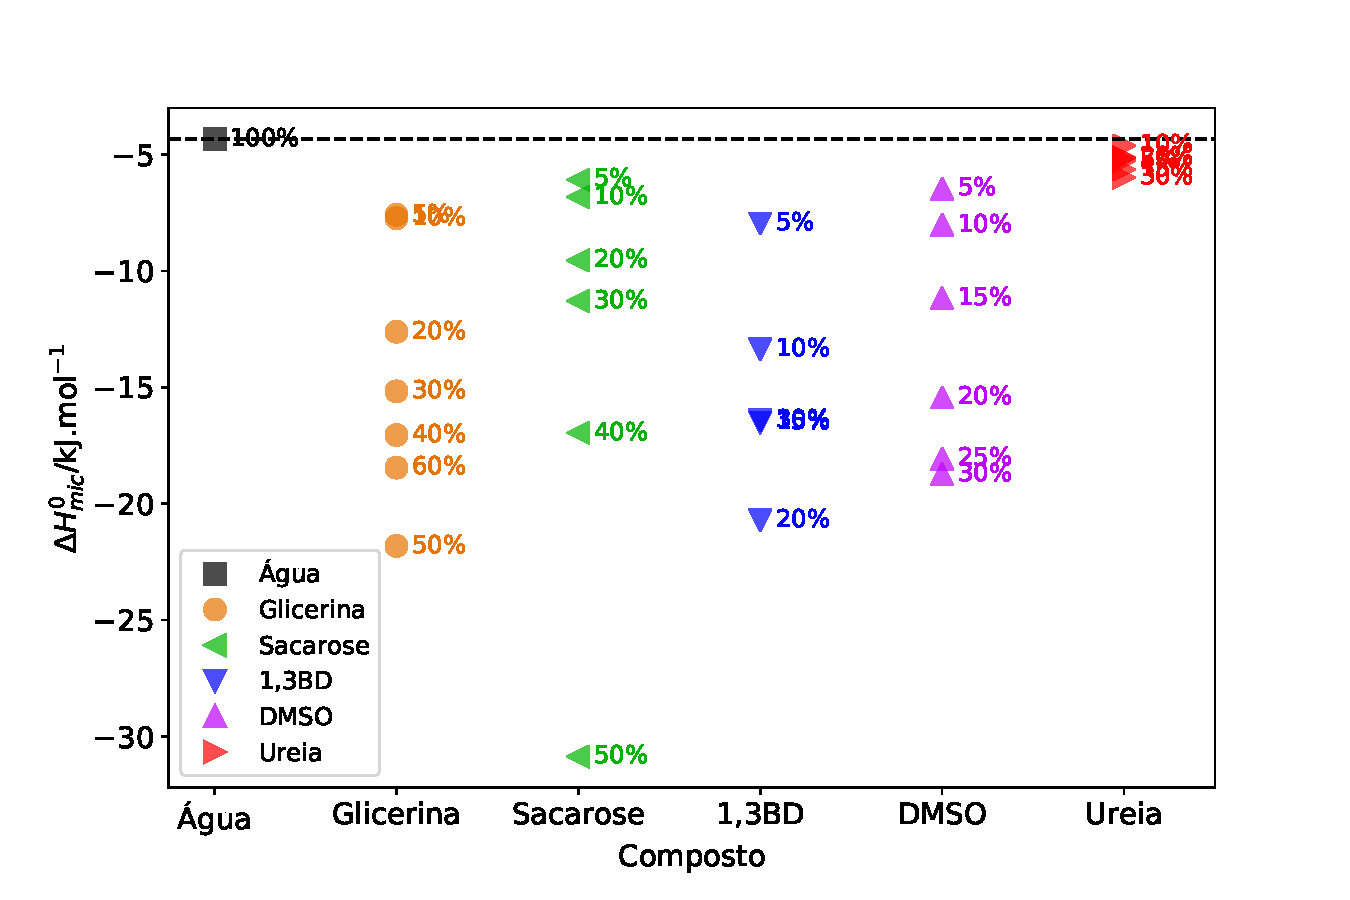
\includegraphics[width=\textwidth]{imagens/itc/DH_por_composto}
%				\caption{\DHmic}
%				\label{fig:dh_por_composto}
%			\end{subfigure}
%		
%			\caption{\cmc{} e \DHmic{} para os vários aditivos}
%			\label{fig:cmc_dh_por_composto}
%		\end{figure}

		\begin{figure}[h]
		%	\centering
			\begin{subfigure}[t]{0.5\textwidth}
				\centering
				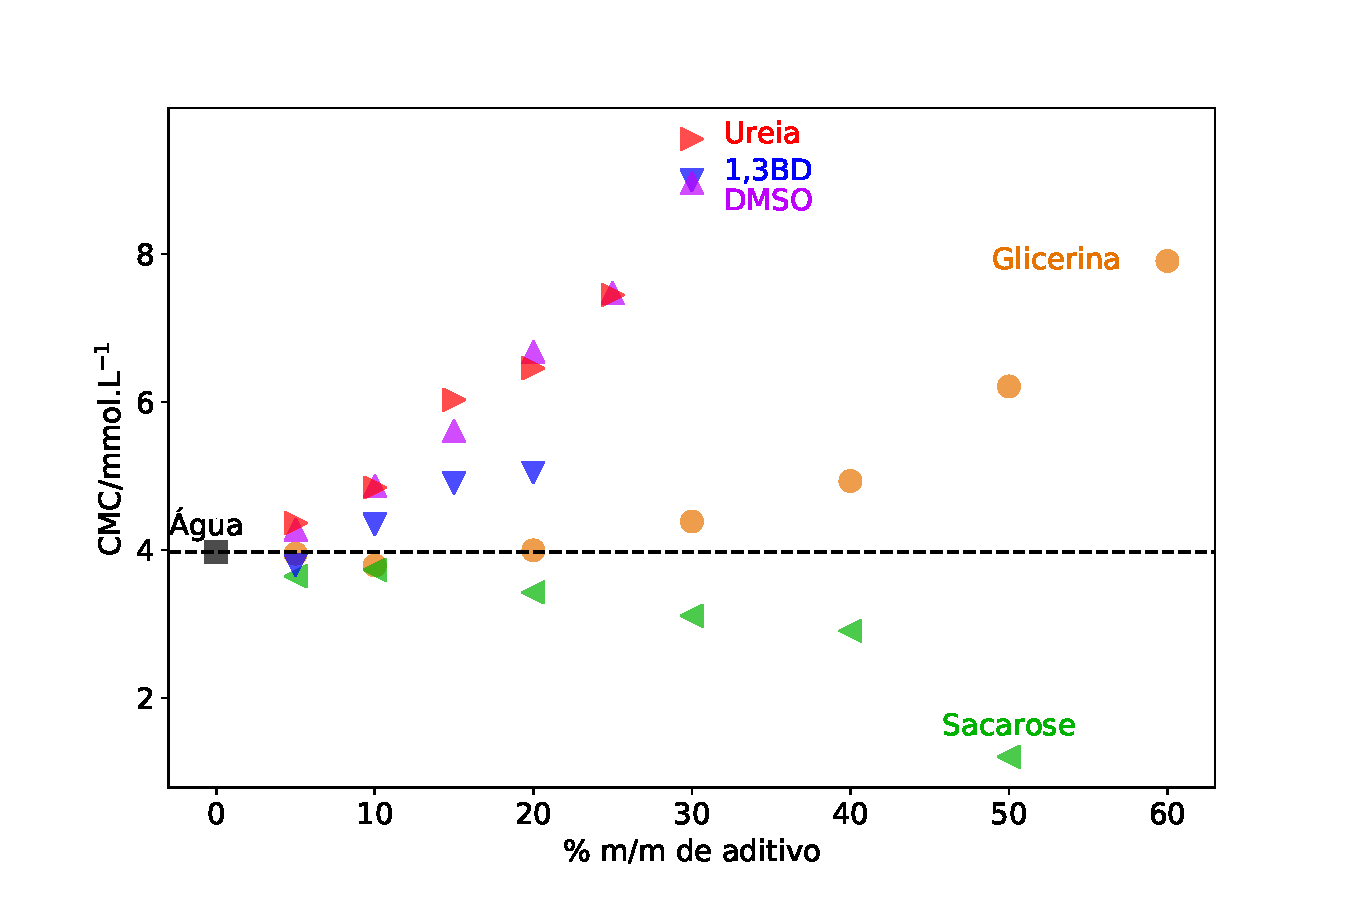
\includegraphics[width=\textwidth]{imagens/itc/ITC_cmc_adit}
				\caption{\cmc}
				\label{fig:cmc_por_conc}
			\end{subfigure} %
			\begin{subfigure}[t]{0.5\textwidth}
				\centering
				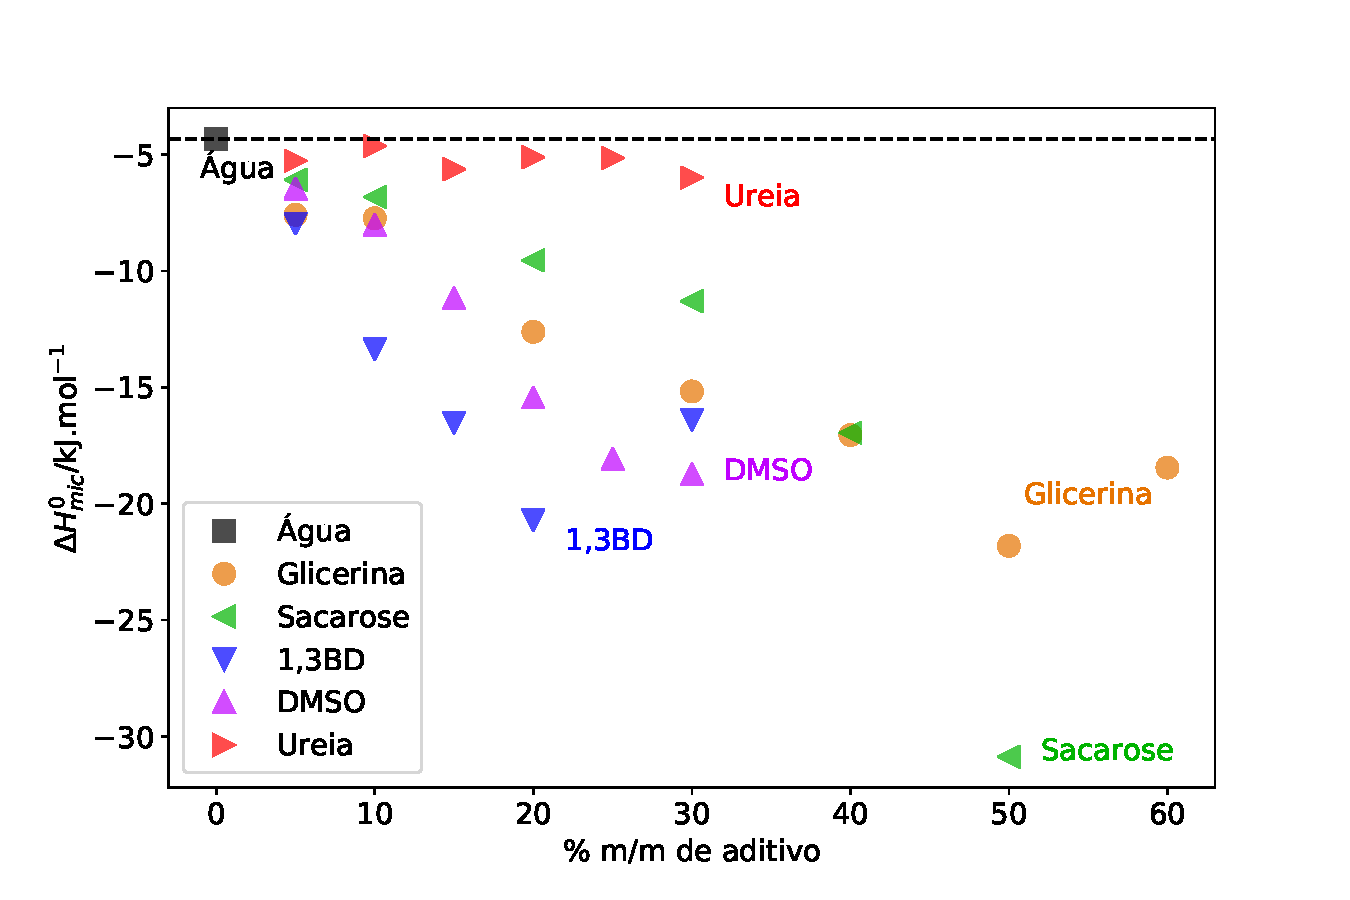
\includegraphics[width=\textwidth]{imagens/itc/ITC_DH_adit}
				\caption{\DHmic}
				\label{fig:dh_por_conc}
			\end{subfigure}
			
			\caption{\cmc{} e \DHmic{} em função da concentração de aditivo.}
			\label{fig:cmc_dh_por_conc}
		\end{figure}
	
		Vemos que a tendência da \autoref{fig:cmc_por_conc} é bastante similar à \autoref{fig:cwlm_por_conc}, com os aditivos seguindo trajetórias bem comportadas. A tendência relativa dos aditivos também é similar, com a sacarose se mantendo mais próxima à linha basal (neste caso, diminuindo a \cmc), seguido da glicerina e os outros três aditivos se agruparam, mostrando que seus efeitos são similares. Já a \autoref{fig:dh_por_conc} é bastante diferente da \autoref{fig:dhwlm_por_conc}, pois aquele demonstra uma clara tendência, praticamente linear para cada aditivo, exceto em altas concentrações, já este, como visto, não possui tendência clara. Isso mostra que a adição de NaSal aumentou a complexidade do sistema. Correlações mais complexas das propriedades com \cwlm, \cmc, \DHwlm{} e \DHmic{} serão apresentadas na página \pageref{sec:PLS_micelizacao}.
	
%				\begin{figure}[h]
%		\begin{subfigure}[t]{0.5\textwidth}
%			\centering
%			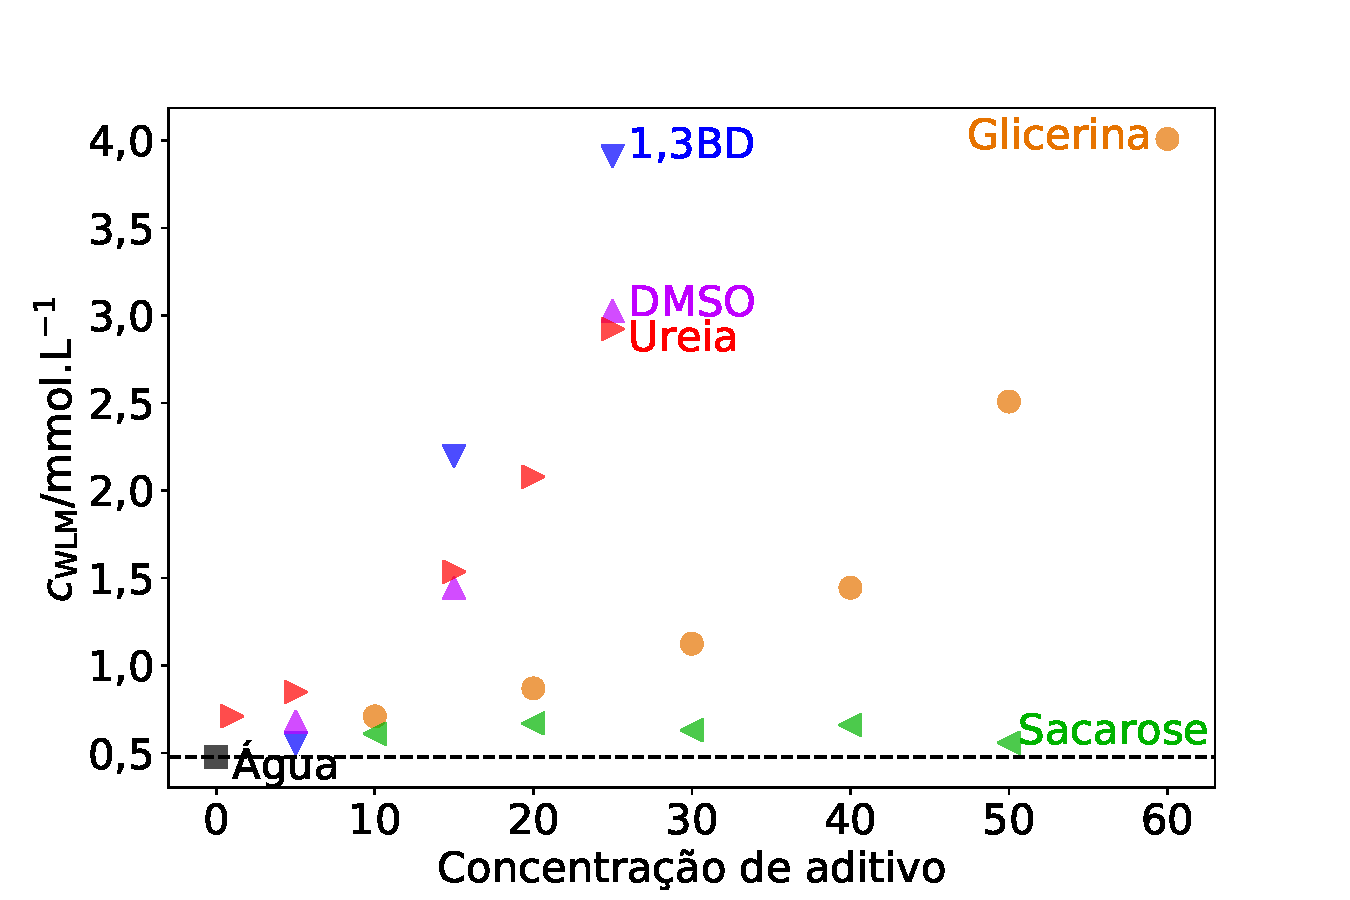
\includegraphics[width=\textwidth]{imagens/itc/Cwlm_por_conc}
%			\caption{\cwlm}
%			\label{fig:cwlm_por_conc}
%		\end{subfigure} %
%		\begin{subfigure}[t]{0.5\textwidth}
%			\centering
%			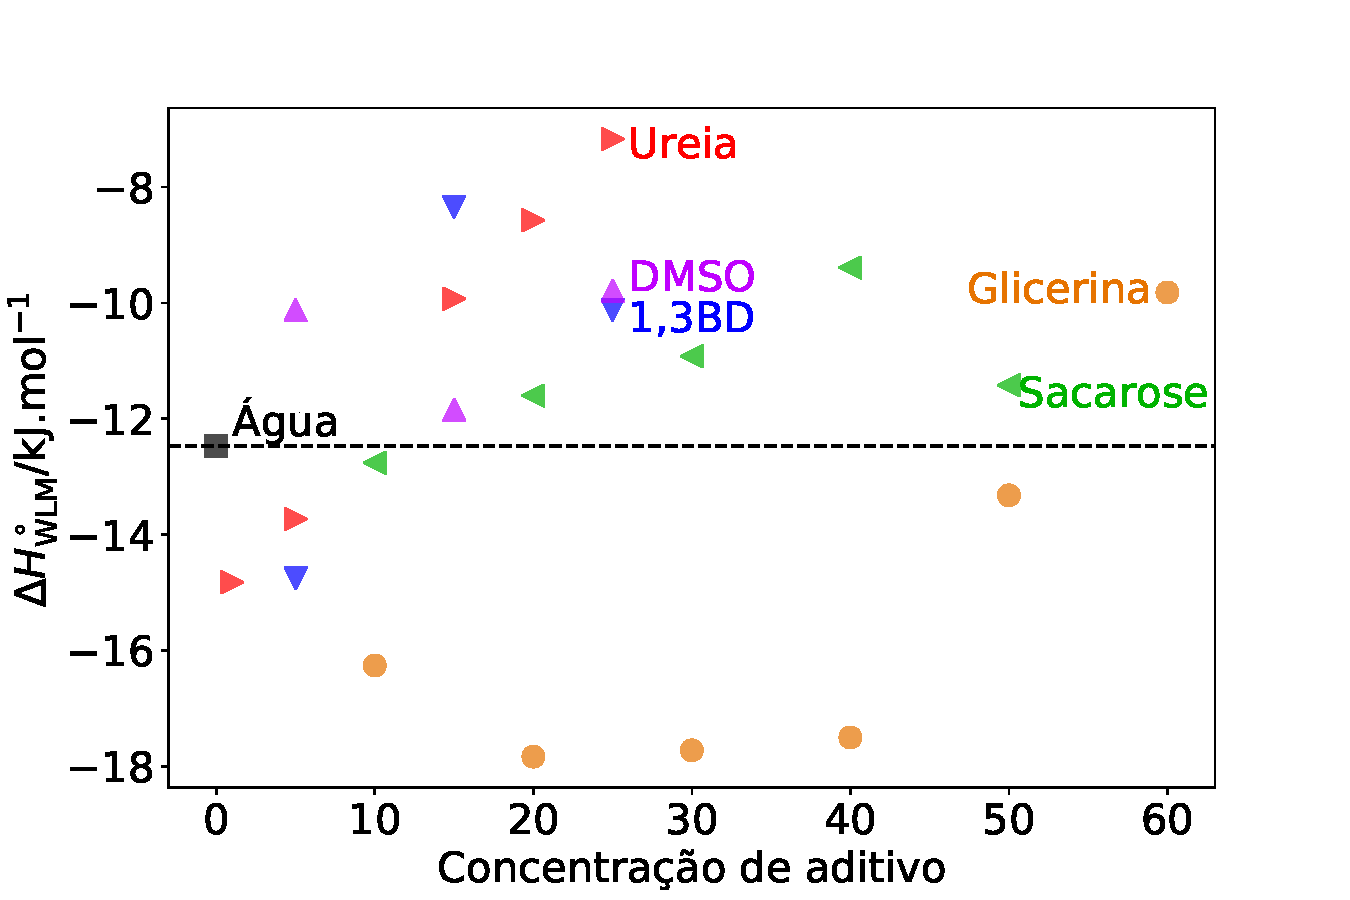
\includegraphics[width=\textwidth]{imagens/itc/DHwlm_por_conc}
%			\caption{\DHwlm}
%			\label{fig:dhwlm_por_conc}
%		\end{subfigure}
%		
%		\caption{\cwlm{} e \DHwlm{} em função da concentração de aditivo para titulações de \TTAB{} em NaSal 1,5 \mM.}
%		\label{fig:cwlm_dhwlm_por_conc}
%	\end{figure}
	
		\FloatBarrier
		
	\chapter{Parâmetros estudados}
	\label{sec:parametros_estudados}
		
		Existem vários parâmetros físico-químicos que descrevem solventes. Inicialmente, o índice de refração foi escolhido com base nos estudos anteriores de Hoffmann, devido à conexão com a constante de Hamaker (\autoref{eqn:constante_hamaker_lifshitz}), que modula a atração/repulsão coloidal (para duas esferas, vide \autoref{eqn:interacao_duas_esferas}). Quanto mais próximos forem os índices de refração entre o solvente e as micelas gigantes, menor será a atração intermicelar. \index{micelas gigantes!constante de Hamaker} \index{resultados!constante de Hamaker}
		
		A constante dielétrica \(\varepsilon\) é um parâmetro relacionado à polaridade do solvente. Quanto maior for a constante dielétrica, mais fracas são as interações eletrostáticas e dipolares (Equações \ref{eqn:potencial_eletrostático}, \ref{eqn:energia_Keesom}, \ref{eqn:energia_Debye}) pois o campo elétrico oposto gerado pelas moléculas do solvente age no sentido contrário do campo elétrico criado por íons e dipolos. Logo, dois íons de cargas opostas não se atraem com tanta facilidade, já que o campo elétrico de um íon decai muito rapidamente, e as forças entrópicas os afastam. Na constante de Hamaker, a contribuição dipolar, que depende da constante dielétrica, é geralmente pequena, e nunca maior que \(\sfrac{3}{4}kT\), porém pode ser relevante na interação de hidrocarbonetos (núcleo micelar) e água.  \index{micelas gigantes!constante dielétrica} \index{resultados!constante dielétrica}
		
		A permissividade dielétrica e o índice de refração estão ambos relacionados pois dependem da polarizabilidade molecular, e de seu momento de dipolo, \(u\). Efeitos adicionais de separação de carga, que podem ocorrer pela estruturação do solvente em ligações de hidrogênio, não são considerados por essa relação. Logo, é interessante utilizar a constante dielétrica, que considera esses efeitos adicionais do solvente, e o índice de refração, que é proporcional somente à polarizabilidade molecular. É possível combinar a constante dielétrica e o momento de dipolo em um fator, chamado de fator eletrostático, \emph{IT}, mas esses parâmetros não foram considerados neste trabalho devido à presença de misturas de solventes, e pela facilidade de se utilizar propriedades do contínuo na interpretação.\cite{ReichardtSolvents}
		
		Dois parâmetros podem ser utilizados para descrever a estruturação de um solvente, a densidade de energia coesiva \(c\) (\autoref{eqn:densidade_energia_coesiva}), e a pressão interna \(\pi\) (\autoref{eqn:pressao_interna}). \cite{ReichardtSolvents}
		% refs [98-100, 175] do cap 3 do livro de propriedades de solvente
		
		\begin{equation}
			c = \dfrac{\Delta U_V}{V_m} = \dfrac{\Delta H_V - R\cdot T}{V_m}
			\label{eqn:densidade_energia_coesiva}
		\end{equation}
		
		\begin{equation}
			\pi = \left( \dfrac{\partial U}{\partial V_m} \right)_T
			\label{eqn:pressao_interna}
		\end{equation}
		
		\noindent onde \(\Delta U_V\) e \(\Delta H_V\) são a energia interna e entalpia de vaporização e \(V_m\) é o volume molar do líquido. A razão de se utilizar a entalpia/energia interna de vaporização é a seguinte. Ao levar um líquido de seu estado condensado para o estado gasoso, todas as ligações líquido-líquido tiveram que ser rompidas. Logo, dividindo-se essa energia pelo volume molar obtemos uma densidade de energia coesiva.\cite{ReichardtSolvents} 
		
		
		A pressão interna, por sua vez, é a energia necessária para abrir uma cavidade no solvente, pois a variação de volume é necessariamente pequena, de modo a acomodar o soluto. Esse parâmetro é resultado das forças atrativas serem mais fortes que as repulsivas, e portanto está mais relacionado às interações dispersivas e dipolo-dipolo. Já \(c\) está relacionado à interações solvente-solvente específicas, como a ligação de hidrogênio.\cite{ReichardtSolvents}
		
		A diferença entre esses dois parâmetros (\(c - \pi\)) fornece uma medida da força das ligações de hidrogênio, e a razão \(n = \sfrac{\pi}{c}\) fornece uma medida da relação entre a força das ligações de hidrogênio e outras atrações. Essa razão se aproxima de 1 para hidrocarbonetos e é próxima de zero para solventes com fortes ligações de hidrogênio. O quadrado de \(c\) é conhecido também como o parâmetro de solubilidade de Hildebrand, \(\delta\). Esse parâmetro foi estendido para sistemas polares, por Hansen.\cite{ReichardtSolvents}
		
		Porém, os solventes utilizados neste trabalho são todos compostos principalmente por água, e em alguns casos os aditivos são sólidos (ureia, sacarose). Além disso, obter esses parâmetros para as misturas não é uma tarefa para qual o laboratório está equipado. Portanto, é necessário utilizar outro parâmetro que esteja relacionado à estruturação do solvente. Um parâmetro relacionado aos parâmetros de Hildebrand e de Hansen, e que já foi previamente utilizado para discutir sistemas micelares,\cite{Moya2007a, Abdel-Rahem2012} é o parâmetro de Gordon\footnote{Não confundir com o módulo no platô \(G\)} \(G\), definido na \autoref{eqn:Gordon}, que é baseado na tensão superficial, \autoref{eqn:tens_superficial}.\cite{ReichardtSolvents}

		\begin{equation}
			G = \dfrac{\gamma}{\overline{V}_m^{\frac{1}{3}}}
			\label{eqn:Gordon}
		\end{equation}
		
		\begin{equation}
			\overline{V}_m = \overline{V}_{m_{1}}\chi_1 + \overline{V}_{m_{2}}\chi_2
			\label{eqn:volume_molar_médio}
		\end{equation}
		
		\noindent onde \(\gamma\) é a tensão superficial do líquido, \(\overline{V}_m\) é o volume molar do líquido que, quando houver mais de um, pode-se utilizar a \autoref{eqn:volume_molar_médio} para calculá-lo, e \(\chi\) é a fração molar. \index{resultados!parâmetro de Gordon}
		
		A razão de se utilizar o parâmetro de Gordon vem de um argumento semelhante ao parâmetro de densidade de energia coesiva. Nesse caso, o aumento da área superficial de um líquido necessita da quebra de interações líquido-líquido das moléculas que vão para a superfície. Um líquido com interações intermoleculares fracas possui uma tensão superficial baixa, pois é fácil quebrar essas ligações. Por outro lado, um líquido com interações intermoleculares fortes, como a água, possui uma tensão superficial bastante alta. Uma grande vantagem de se utilizar o parâmetro de Gordon é que as medidas de tensão superficial de misturas são facilmente realizadas, necessitando então somente a conversão de \(\gamma\) para \(G\). Porém, \citeauthor{ReichardtSolvents} nota que \(c\) é um parâmetro melhor para descrever a energia coesiva. Isso se torna especialmente evidente quando há aditivos com atividade superficial.

		\section{Índice de refração} \index{resultados!índice de refração \(n\)}
		
		A \autoref{fig:indice_refracao} mostrou como o índice de refração varia com a concentração de aditivo. Como os resultados reológicos evidenciaram, considerar somente o índice de refração não é uma maneira muito boa para explicar o comportamento reológico. Caso contrário, haveria um padrão notável num gráfico comparativo das concentrações e entalpias. Isso está evidenciado nas Figuras \ref{fig:cwlm_dhwlm_por_n} e \ref{fig:cmc_dh_por_n}, onde não há um padrão geral observado para todos os aditivos.
		
		\begin{figure}[h]
			\begin{subfigure}[t]{0.5\textwidth}
				\centering
				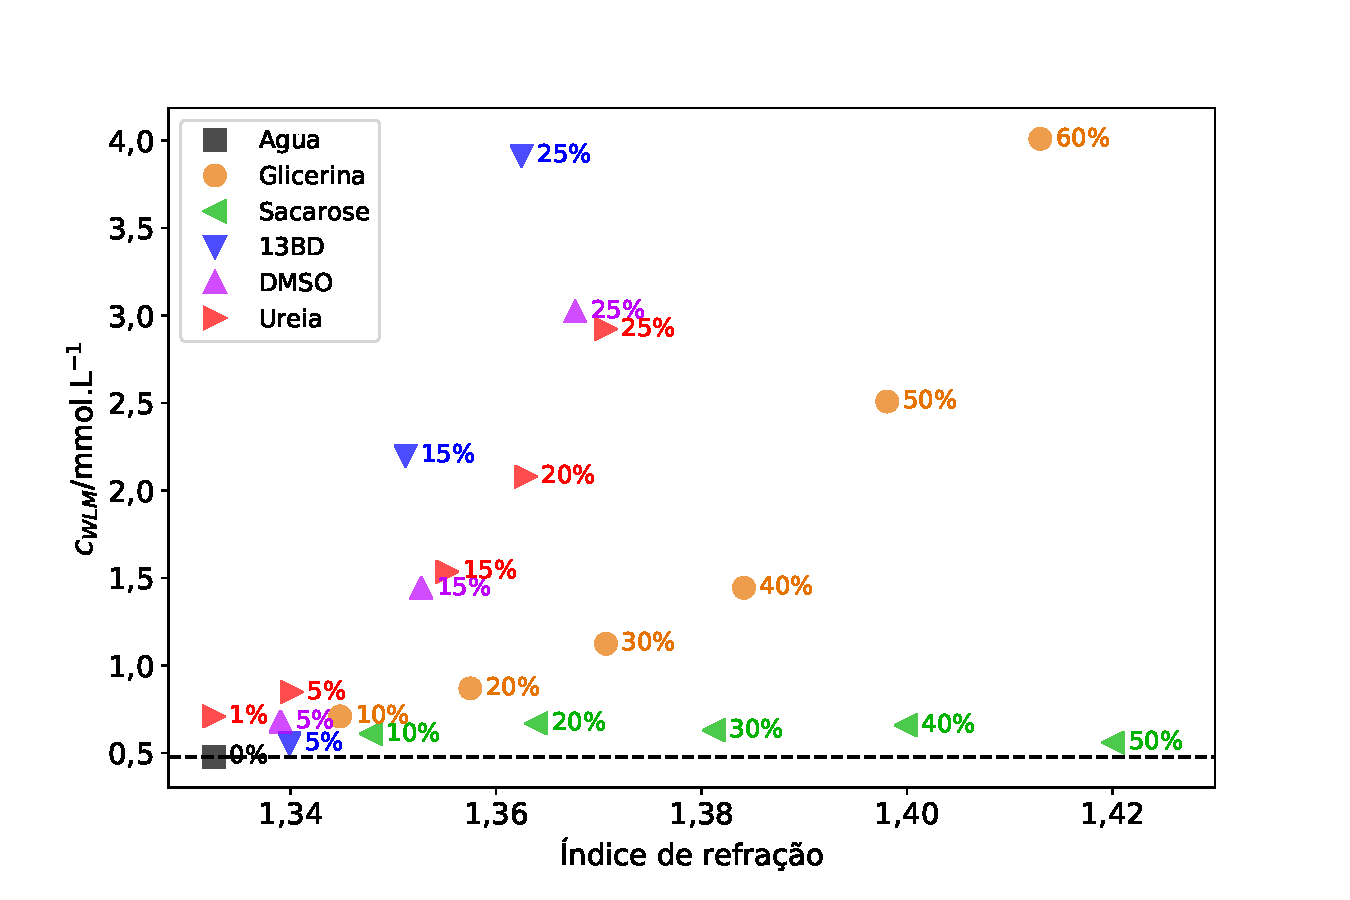
\includegraphics[width=\textwidth]{imagens/itc/Cwlm_por_n}
				\caption{\cwlm}
				\label{fig:cwlm_por_n}
			\end{subfigure} %
			\begin{subfigure}[t]{0.5\textwidth}
				\centering
				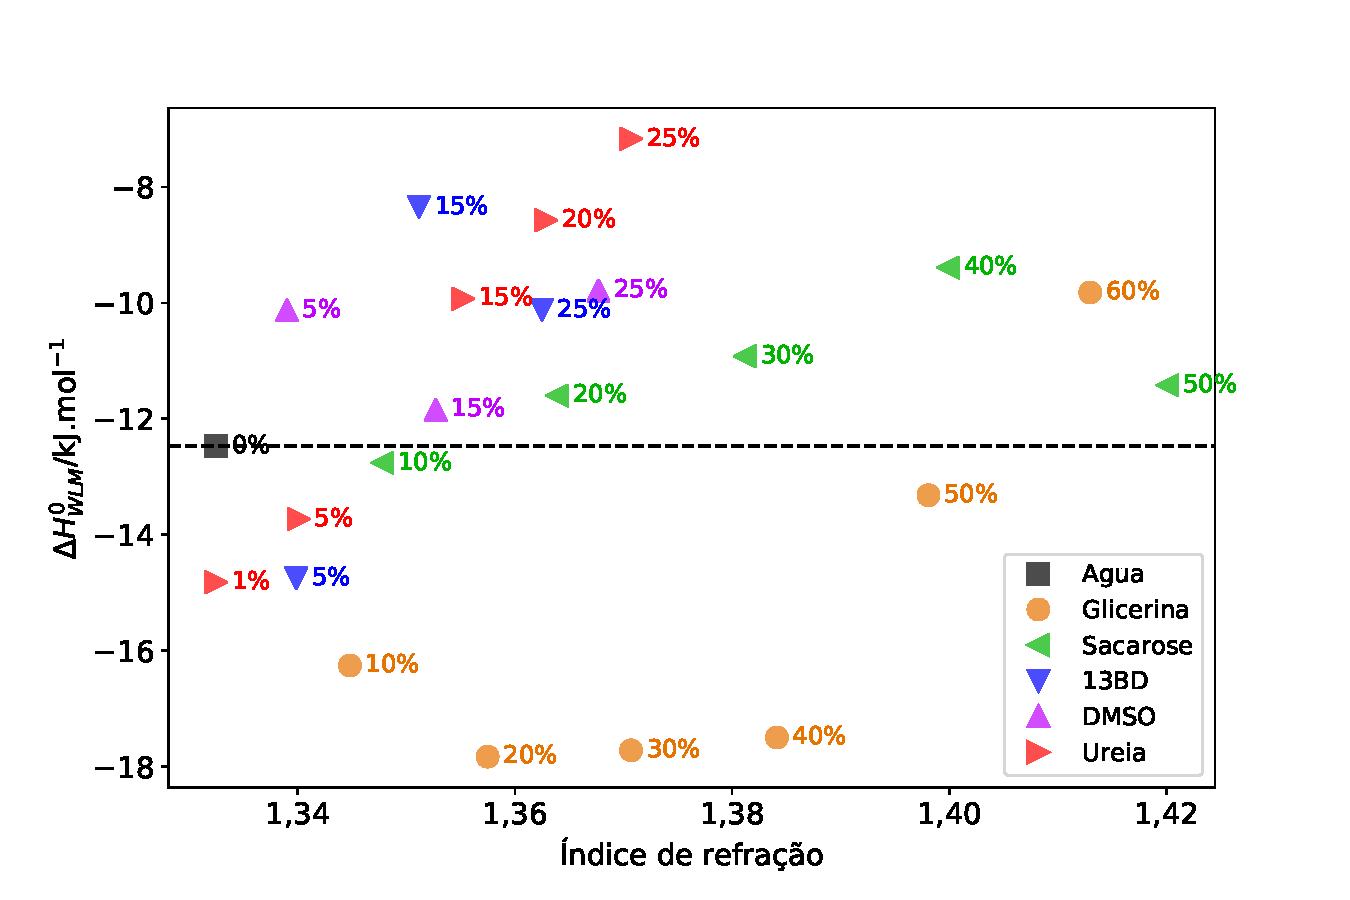
\includegraphics[width=\textwidth]{imagens/itc/DHwlm_por_n}
				\caption{\DHwlm}
				\label{fig:dhwlm_por_n}
			\end{subfigure}
			
			\caption{\cwlm{} e \DHwlm{} em função do índice de refração. A reta tracejada indica os resultados para a água pura.}
			\label{fig:cwlm_dhwlm_por_n}
		\end{figure}
		
		\begin{figure}[h]
			\begin{subfigure}[t]{0.5\textwidth}
				\centering
				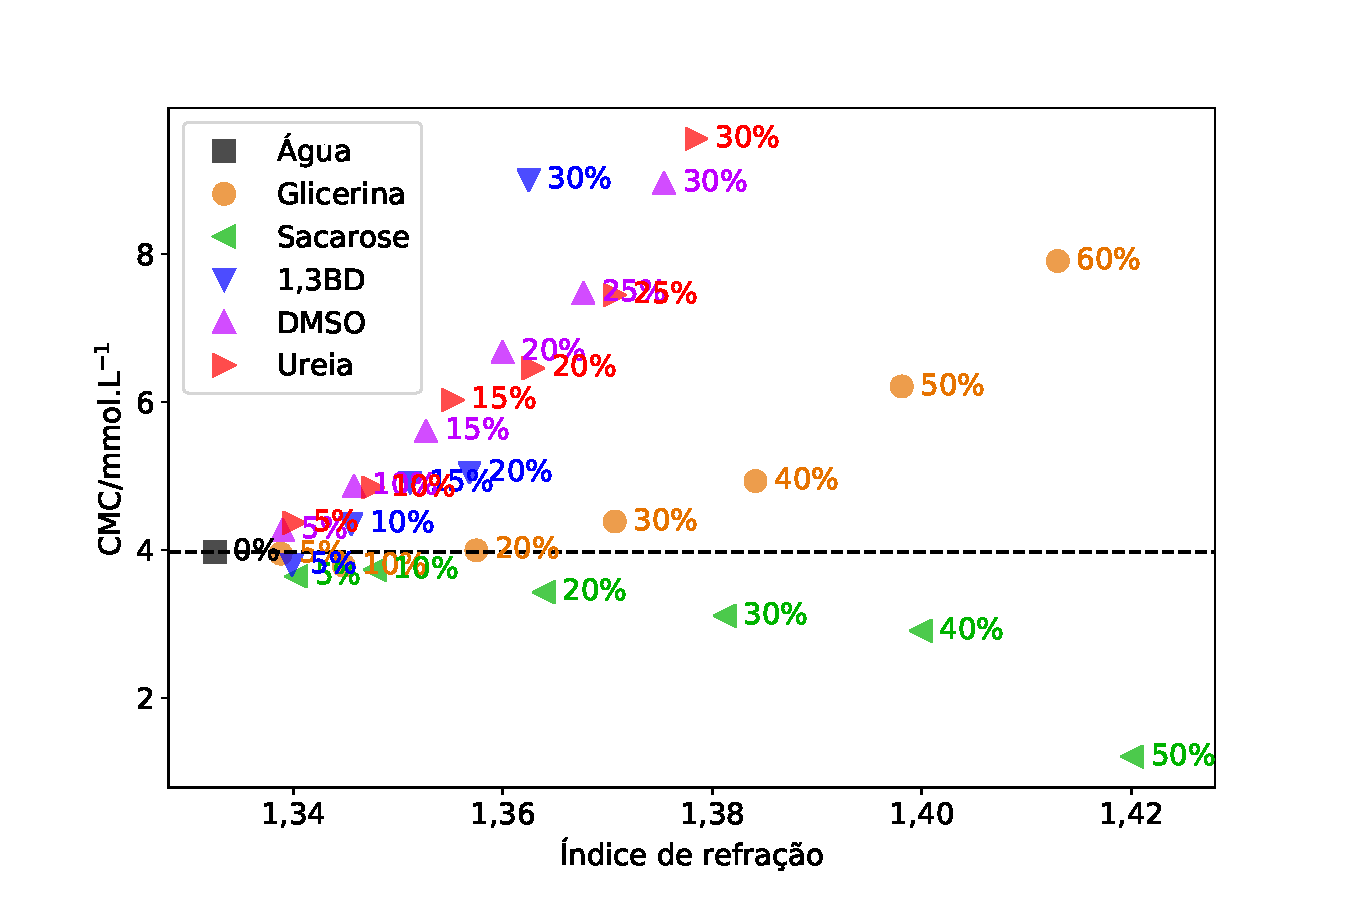
\includegraphics[width=\textwidth]{imagens/itc/CMC_por_n}
				\caption{\cmc}
				\label{fig:cmc_por_n}
			\end{subfigure} %
			\begin{subfigure}[t]{0.5\textwidth}
				\centering
				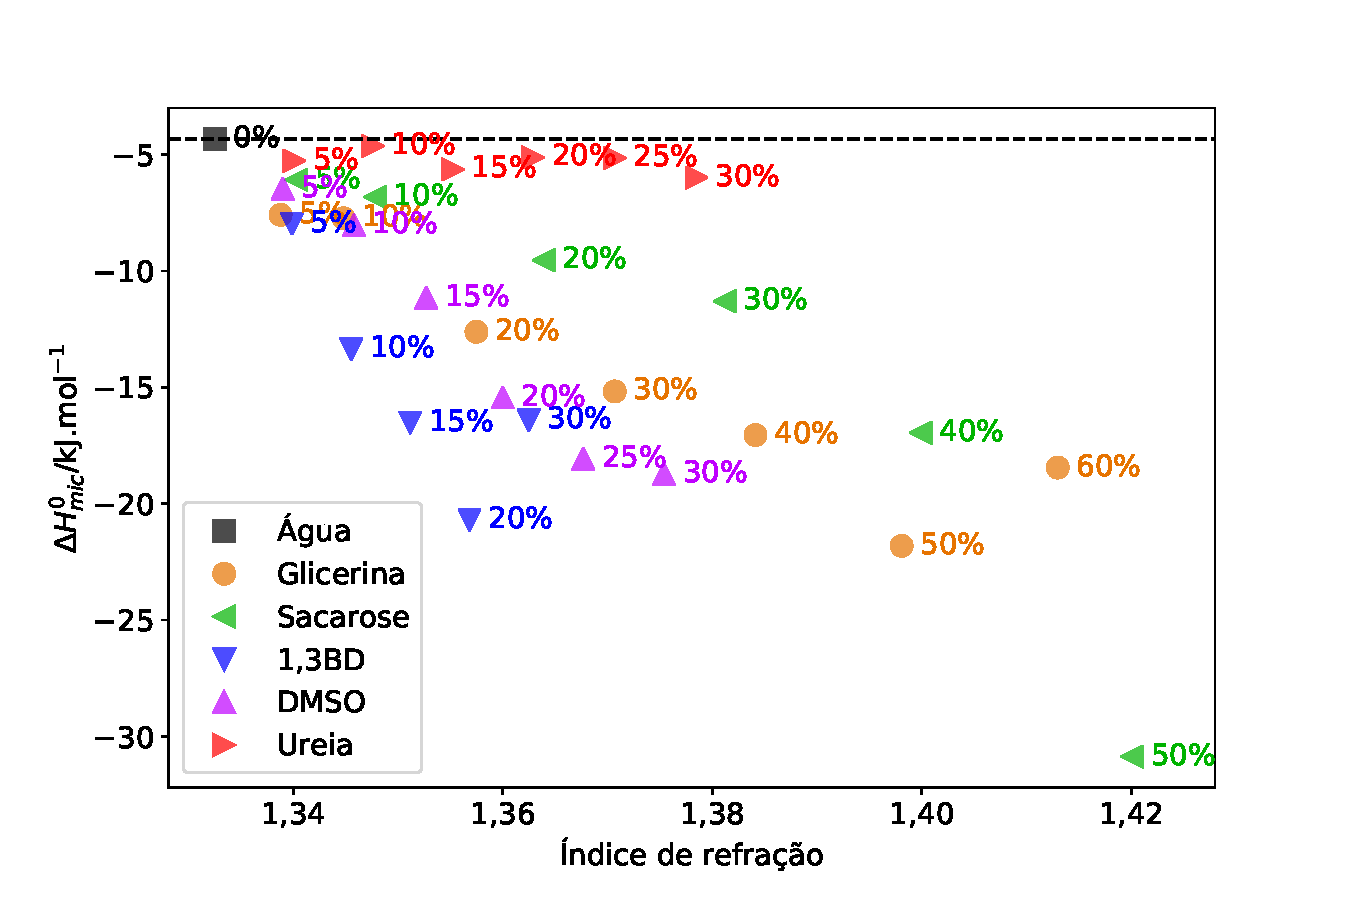
\includegraphics[width=\textwidth]{imagens/itc/DH_por_n}
				\caption{\DHmic}
				\label{fig:dh_por_n}
			\end{subfigure}
			
			\caption{\cmc{} e \DHmic{} em função do índice de refração.  A reta tracejada indica os resultados para a água pura.}
			\label{fig:cmc_dh_por_n}
		\end{figure}

		Comparando-se as Figuras \ref{fig:cwlm_dhwlm_por_n} e \ref{fig:cmc_dh_por_n}, pode-se observar que há uma correlação entre as \cmc{} e \cwlm. Aparentemente há um grupo composto de \BD, DMSO e ureia. Glicerina e sacarose desviam-se significativamente, sendo que sacarose possui o comportamento mais diferenciado, não havendo mudança na \cwlm{} e uma diminuição da \cmc{}.
		
		Agrupamentos desse tipo não podem ser feitos com as entalpias, que parecem ter valores bastante variáveis. Porém, é necessário enfatizar que os valores de entalpia obtidos para a formação de micelas gigantes não são tão confiáveis quanto os de formação de micelas esféricas. Para obter os perfis completos de formação de micelas gigantes, foi necessário aumentar a concentração de surfactante na seringa. Isso reduz a precisão na região inicial do perfil, onde é calculado o \DHwlm. Além disso, a resolução dos entalpogramas obtidos pelo calorímetro PEAQ é menor (39 pontos) do que no VP-ITC (90 pontos). Esse problema possui menor relevância para \cwlm{}, que foi definida como sendo o ponto mínimo da curva, não uma subtração de duas regiões pré e pós-micelar.  Apesar disso, o padrão observado para as mudanças de entalpia na presença de ureia podem ser explicadas pelo aumento da constante dielétrica do meio, como previamente mencionado.
	
		É interessante notar que as figuras que comparam as concentrações de formação e entalpias com o índice de refração (Figuras \ref{fig:cwlm_dhwlm_por_conc} e \ref{fig:cwlm_dhwlm_por_n}, \ref{fig:cmc_dh_por_conc} e \ref{fig:cmc_dh_por_n}) e a concentração de aditivo são bastante semelhantes. Isso se deve à dependência praticamente linear em baixas concentrações do índice de refração com a concentração de aditivo na escala mássica, um dos motivos para essa escala ser escolhida.
		
		\FloatBarrier
		
		\section{Constante dielétrica} \index{resultados!constante dielétrica \(\varepsilon\)}
		
		A constante dielétrica está relacionada ao grau de dissociação de espécies iônicas em solução. Quanto maior a constante, maior o grau de dissociação. Isso resulta, por exemplo, no aumento da \cmc{} pois há menos contraíons para reduzir a carga superficial micelar. A contribuição desse parâmetro já havia sido levantada em um estudo anterior.\cite{Abdel-Rahem2012}
		A \autoref{fig:cte_dieletrica} mostra como a constante dielétrica varia em função da concentração de aditivo.
		
		\begin{figure}[h]
			\centering
			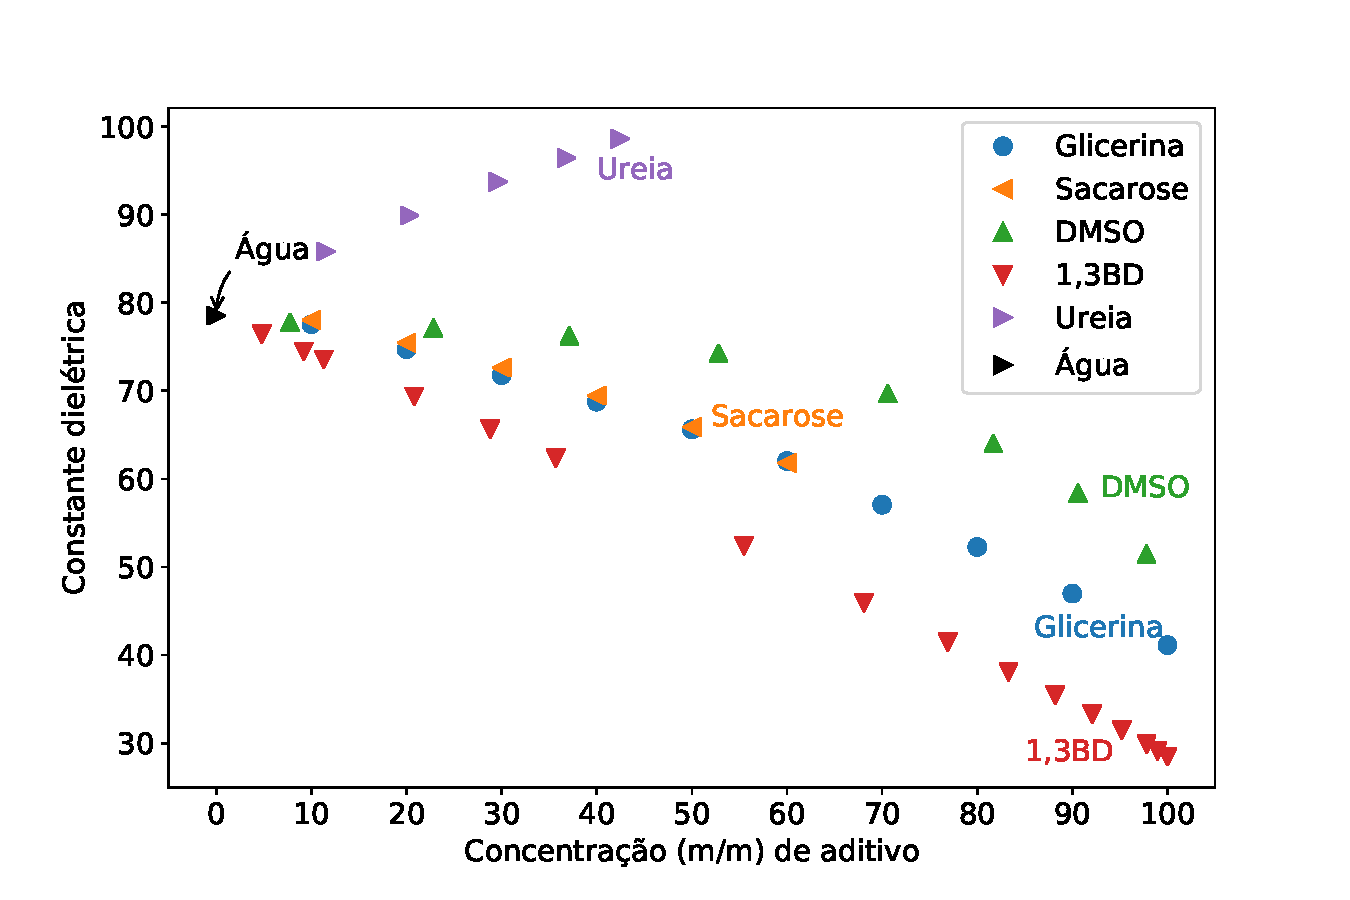
\includegraphics[width=0.7\textwidth]{imagens/propriedades/cte_dieletrica}
			\caption{Constante dielétrica em função da concentração de sacarose,\cite{Malmberg1950a} DMSO,\cite{Kaatze1989a} \BD,\cite{Piekarski1995} ureia\cite{Wyman1933} a 25°C, e glicerina a 20°C.\cite{Akerlof1932}}  % ureia: 25°C. DMSO: 25°C, sacarose: 25°C, Glicerina:20°C, 1,3BD:25°C
			\label{fig:cte_dieletrica}
		\end{figure}
	
		Não há variação entre o comportamento da sacarose e glicerina, e o DMSO praticamente não afeta a constante dielétrica na faixa de concentração estudada. O \BD{} possui sempre os menores valores de \(\varepsilon\), o que indica que nessas soluções há a menor dessorção de contraíons da superfície micelar. O aditivo que afeta a constante dielétrica mais diferentemente dos outros é a ureia, que aumenta \(\varepsilon\). Isso se mostrará crucial para explicar seu comportamento diferenciado.
	
		É possível que, com a dessorção de \Sal{} das micelas, as amostras com maior concentração de ureia se tornem mais carregadas positivamente. Logo, a formação de uma rede ramificada de micelas é menos favorável, pela carga superficial. Por essa razão, não se observa a região intermediária de viscosidade menor, e a viscosidade observada é próxima àquela do sistema altamente carregado.
		
		Os outros aditivos agem de maneira contrária, porém, a quantidade de \Sal{} incorporado já é bastante alta, então a ação de incorporar mais salicilato não tem um efeito tão forte. % todo: achar ref que fala do grau de incorporação de nasal.
		Todavia, ainda é necessário considerar se o aumento da hidrofobicidade do solvente acarretaria numa dessorção de salicilato, apesar de que, devido à sua carga, sua interação com a superfície micelar deve ser mais forte em solventes mais apolares.
	
		Da mesma maneira que o índice de refração, os parâmetros dos ITCs serão comparados com a constante dielétrica do meio para tentar observar algum padrão. Essas comparações estão na \autoref{fig:cwlm_dhwlm_por_eps} e \autoref{fig:cmc_dh_por_eps}.

		
		Algumas observações podem ser feitas quanto aos resultados observados. Aparentemente todos os aditivos possuem uma divergência única do ponto inicial, água, não havendo muita correlação entre eles, com exceção da \DHmic{}, onde a glicerina, sacarose e \BD{} aparentam seguir uma tendência semelhante. A ureia, em todos os casos, diverge pois seu valor de constante dielétrica aumenta. O DMSO não afeta grandemente \(\varepsilon\), mas tanto as concentrações quanto entalpias são fortemente afetadas pelo aumento de sua concentração. Isso indica que a constante dielétrica, por si só, também não consegue explicar os fenômenos observados. Porém, ela é necessária para capturar a divergência observada com a ureia.
		
		\begin{figure}[h]
			\begin{subfigure}[t]{0.5\textwidth}
				\centering
				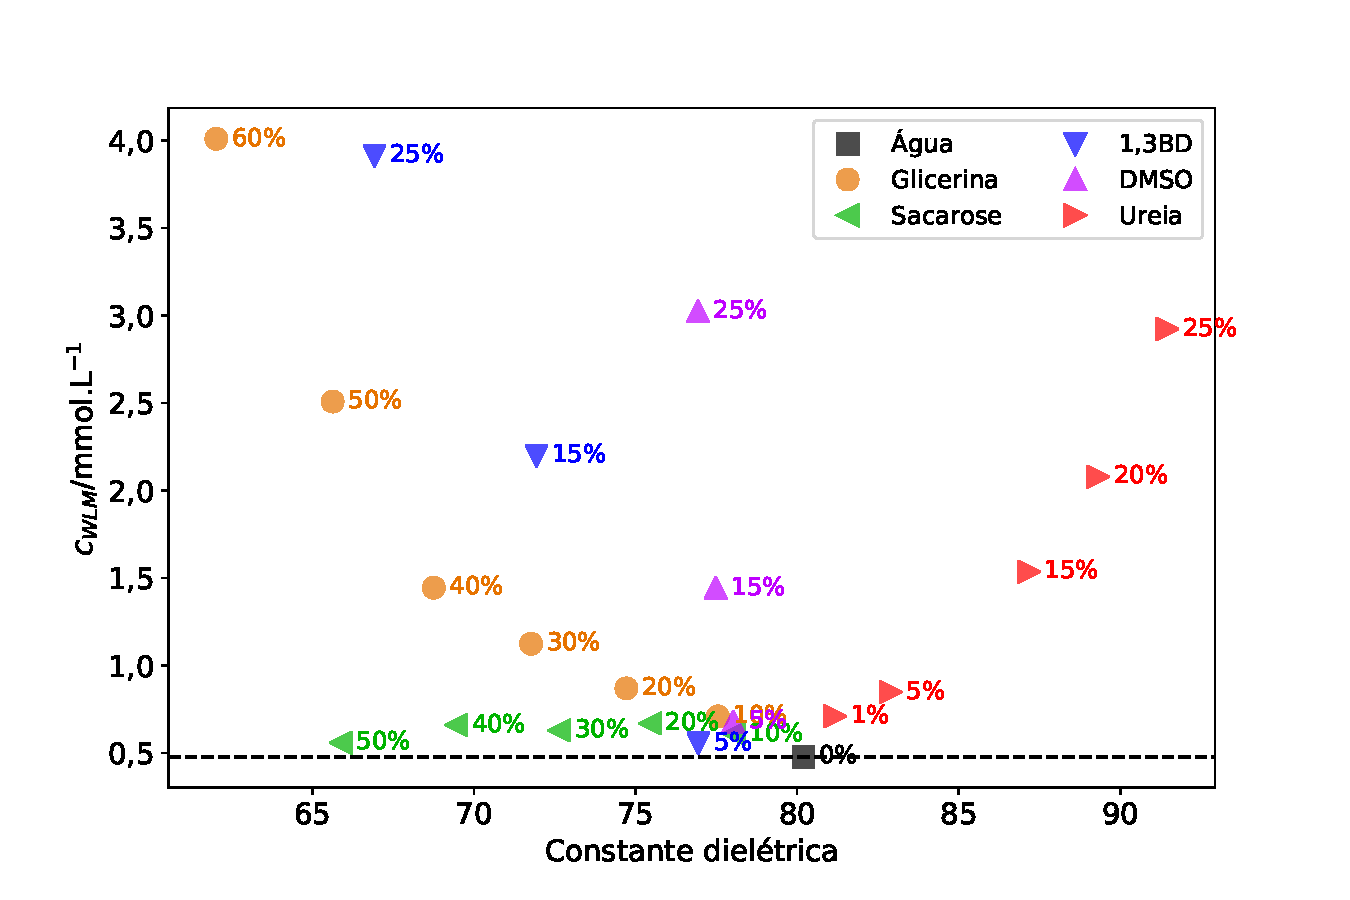
\includegraphics[width=\textwidth]{imagens/itc/Cwlm_por_eps}
				\caption{\cwlm}
				\label{fig:cwlm_por_eps}
			\end{subfigure} %
			\begin{subfigure}[t]{0.5\textwidth}
				\centering
				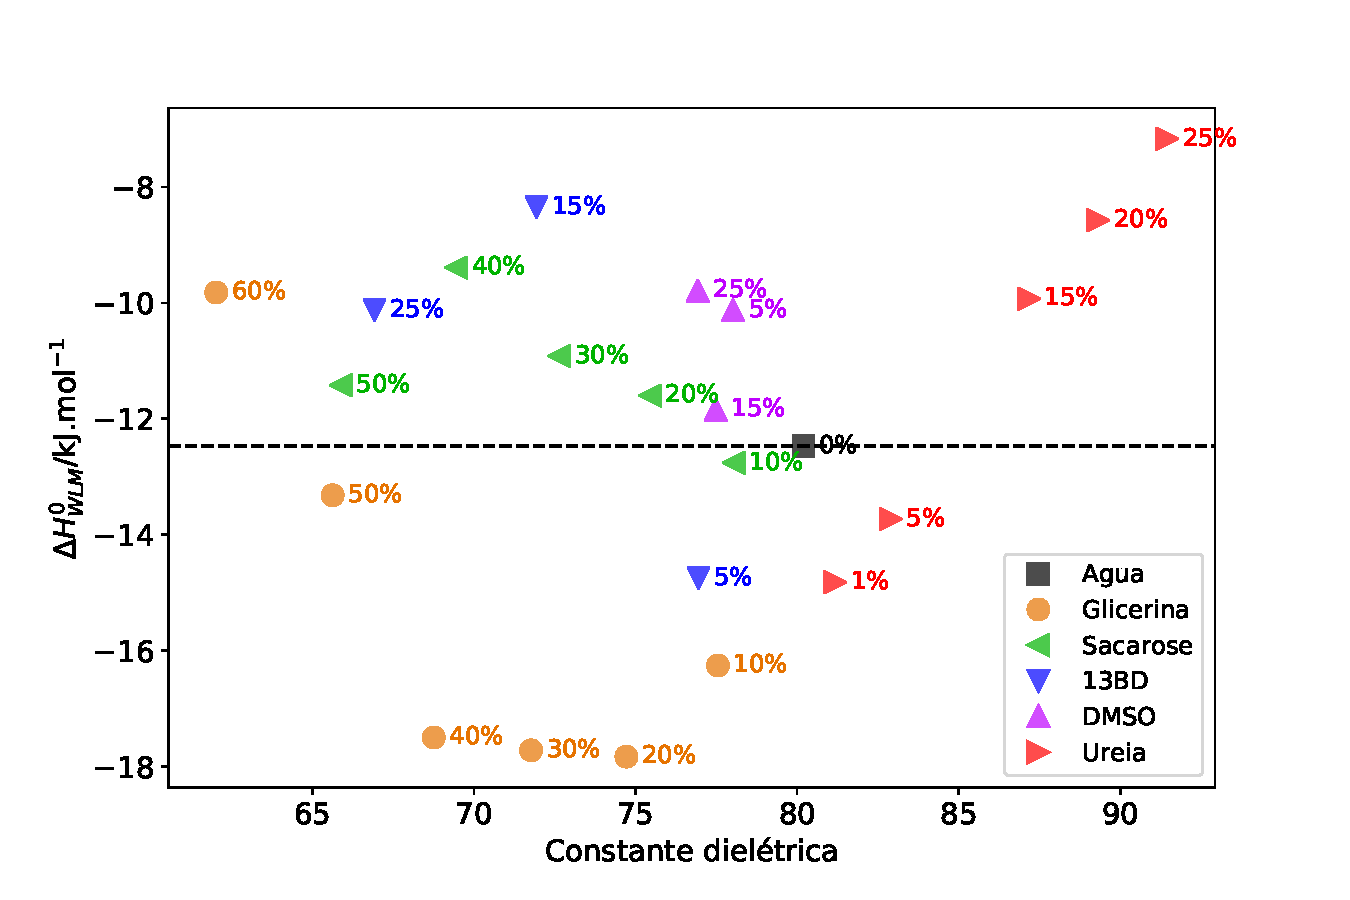
\includegraphics[width=\textwidth]{imagens/itc/DHwlm_por_eps}
				\caption{\DHwlm}
				\label{fig:dhwlm_por_eps}
			\end{subfigure}
			
			\caption{\cwlm{} e \DHwlm{} em função da constante dielétrica \(\varepsilon\).}
			\label{fig:cwlm_dhwlm_por_eps}
		\end{figure}
		
		\begin{figure}[h]
			\begin{subfigure}[t]{0.5\textwidth}
				\centering
				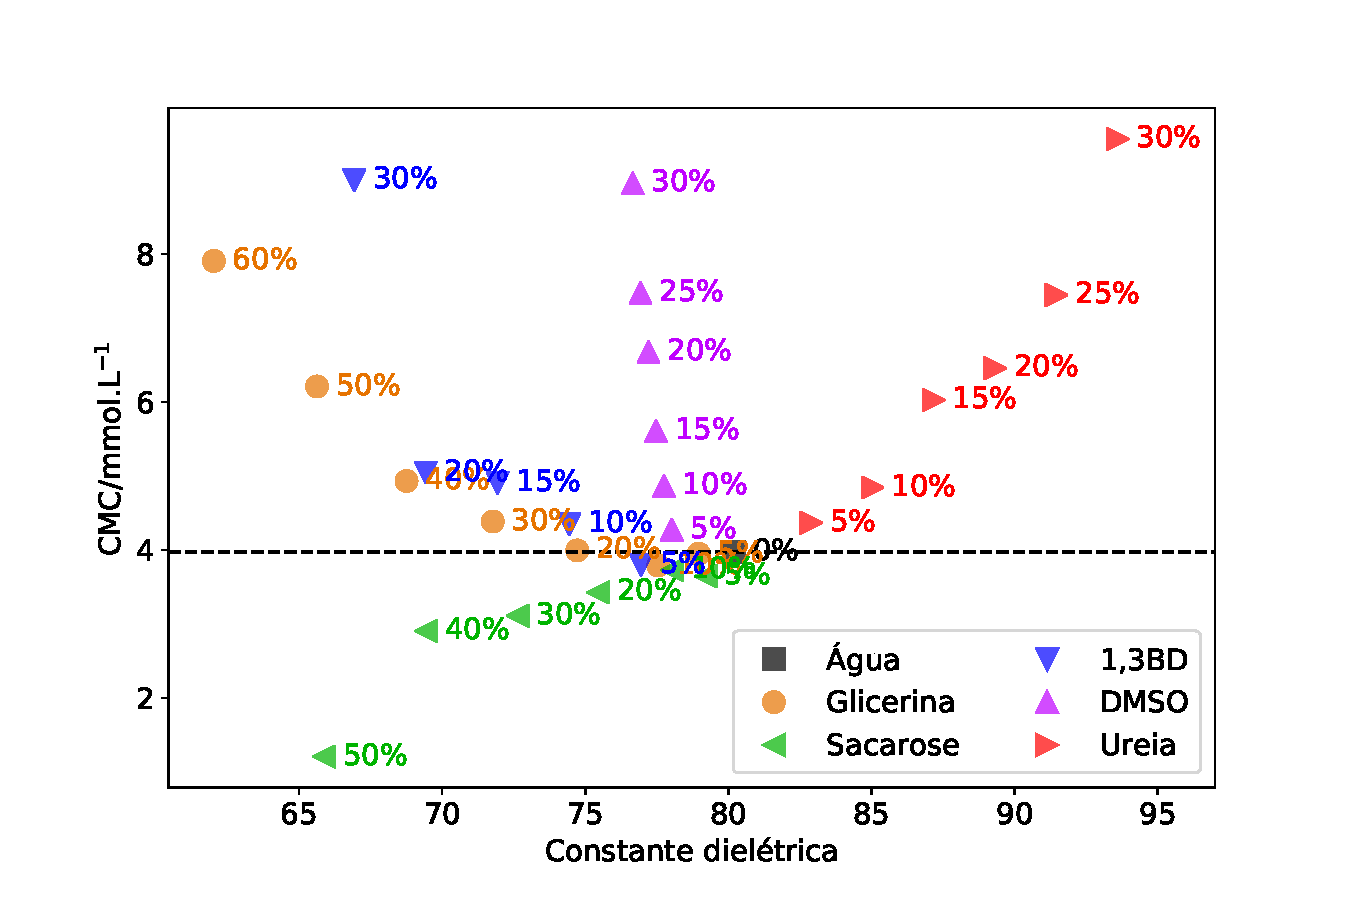
\includegraphics[width=\textwidth]{imagens/itc/CMC_por_eps}
				\caption{\cmc}
				\label{fig:cmc_por_eps}
			\end{subfigure} %
			\begin{subfigure}[t]{0.5\textwidth}
				\centering
				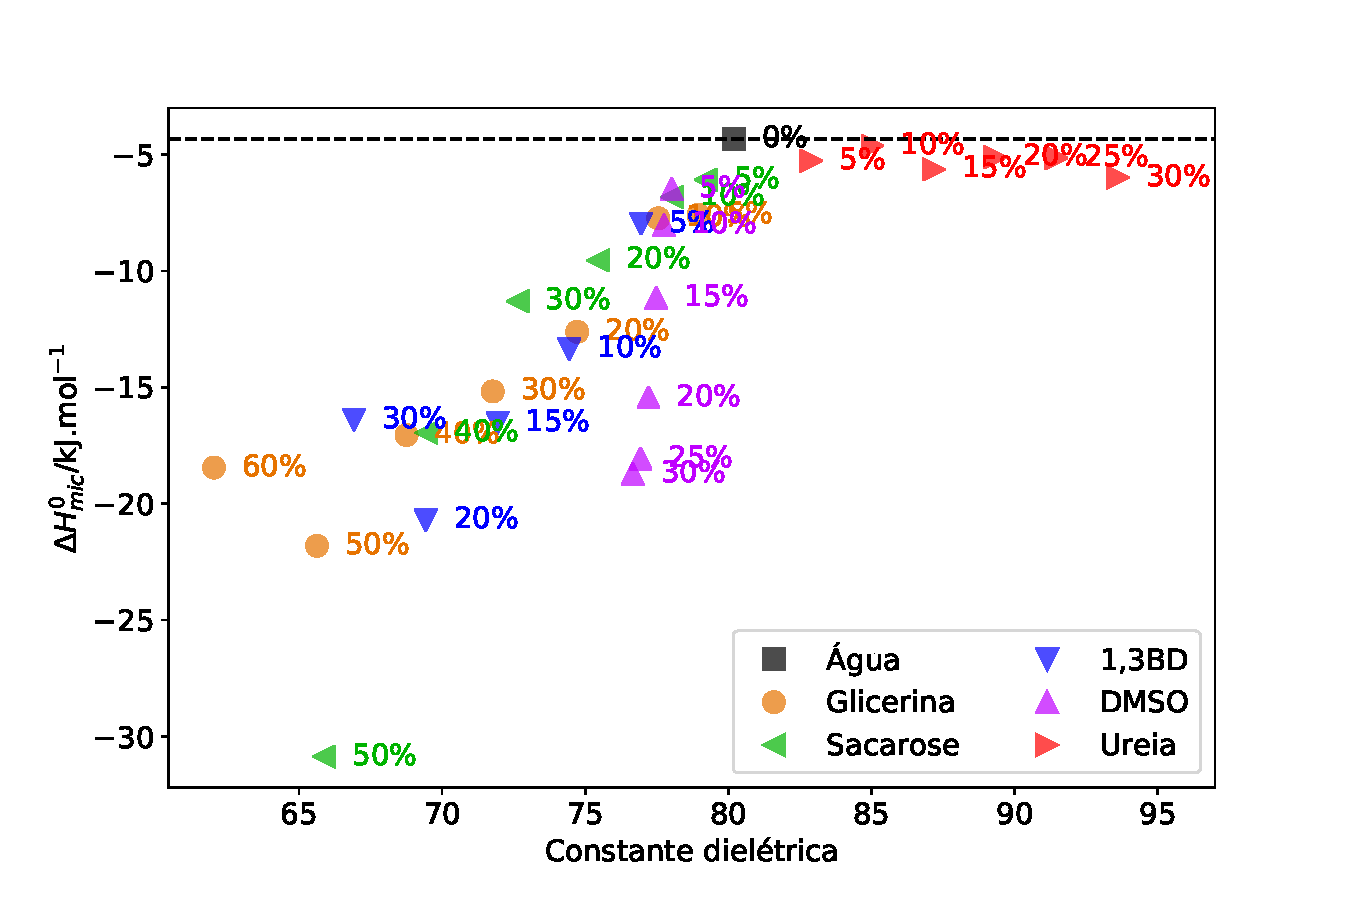
\includegraphics[width=\textwidth]{imagens/itc/DH_por_eps}
				\caption{\DHmic}
				\label{fig:dh_por_eps}
			\end{subfigure}
			\caption{\cmc{} e \DHmic{} em função da constante dielétrica \(\varepsilon\) do meio.}
			\label{fig:cmc_dh_por_eps}
		\end{figure}
		
		\FloatBarrier
		
		\section{Coesão do solvente e Parâmetro de Gordon} \index{resultados!coesão do solvente} \index{resultados!parâmetro de Gordon}
		
		Devido à incapacidade dos outros parâmetros explicarem o comportamento reológico e calorimétrico, procuramos por outras propriedades que possam estar relacionadas. Consultando trabalhos anteriores, pensamos na coesão do solvente para explicar o comportamento reológico e calorimétrico. Solventes bastante estruturados, como a água, diminuem a \cmc{} devido ao aumento da penalidade entrópica. Além disso, estipulamos que solventes mais bem estruturados devem dificultar a locomoção das micelas gigantes durante os processos de reptação, aumentando a viscosidade aparente. A partir disso, foram coletadas informações sobre a coesão dos solventes utilizados.
		
		Glicerina na concentração de 43\% (m/m) possui uma probabilidade reduzida de ligações de hidrogênio, portanto a percolação da rede de ligações de hidrogênio é encurtada.\cite{Parsons2001a, Dashnau2006}. Já açúcares são desestruturadores em baixas concentrações e estruturadores em altas. Para a glicose, a estruturação acontece em torno de 25-30\% m/m,\cite{Giangiacomo2006} já outros estudos mencionam 37\% (m/m).\cite{Ueberreiter1982} Sacarose foi descrita em trabalhos anteriores \cite{Song2008a} como aditivo para aumento da separação interlamelar, semelhante à glicerina. É possível que a sacarose afete as micelas e não as bicamadas devido à maior área de contato das micelas com o solvente. Além disso, a reologia observa a dinâmica das micelas ao fluir pelo solvente, já a distância interlamelar é uma propriedade estática, e seria melhor comparada com uma distância intermicelar média.
		
		DMSO foi demonstrado como um agente desestruturador em altas concentrações e estruturador em baixas, e essas propriedades foram descritas como fracas frente à capacidade do DMSO em solubilizar moléculas de surfactante.\cite{Bertoluzza1979b}
		Já o papel da ureia é inconclusivo de acordo com a literatura, com três mecanismos propostos em estudos,\cite{Dias2002} a saber, um mecanismo direto, um mecanismo indireto, e simplesmente um solvente mais polar. O mecanismo direto estabelece que ligações de hidrogênio favoráveis entre água e ureia contribuem para a troca de moléculas de solvente ao redor de regiões hidrofóbicas, aumentando sua solubilidade. O mecanismo indireto se baseia na desestruturação da água, diminuindo o custo energético/penalidade entrópica para solubilizar grupos apolares. O terceiro mecanismo propõe que a ureia aumenta a estabilidade de íons livres e grupos polares em solução devido ao aumento da constante dielétrica do meio.\cite{Dias2002}
		
		Para seguir a lógica das discussões na outra seção, é necessário levantar uma propriedade que traduza o conceito de coesão do solvente para um número mensurável. O parâmetro de Gordon já foi utilizado na literatura com esse propósito, então ele será utilizado neste trabalho.\cite{Moya2007a, Abdel-Rahem2012} Não foi utilizado o parâmetro de densidade de energia coesiva \(c\) devido à dificuldade de medir esse parâmetro. Porém, é necessário reforçar que \(G\) não traduz perfeitamente o conceito de estruturação, e será utilizado mais como uma maneira para facilitar a discussão. O parâmetro de Gordon já foi definido na \autoref{eqn:Gordon}.
		
		As tensões superficiais obtidas estão na \autoref{fig:tensao_superficial_por_conc} e os valores do parâmetro de Gordon calculados estão na \autoref{fig:param_gordon_por_conc}. \index{resultados!tensão superficial}
		
		\begin{figure}[h]
			\centering
			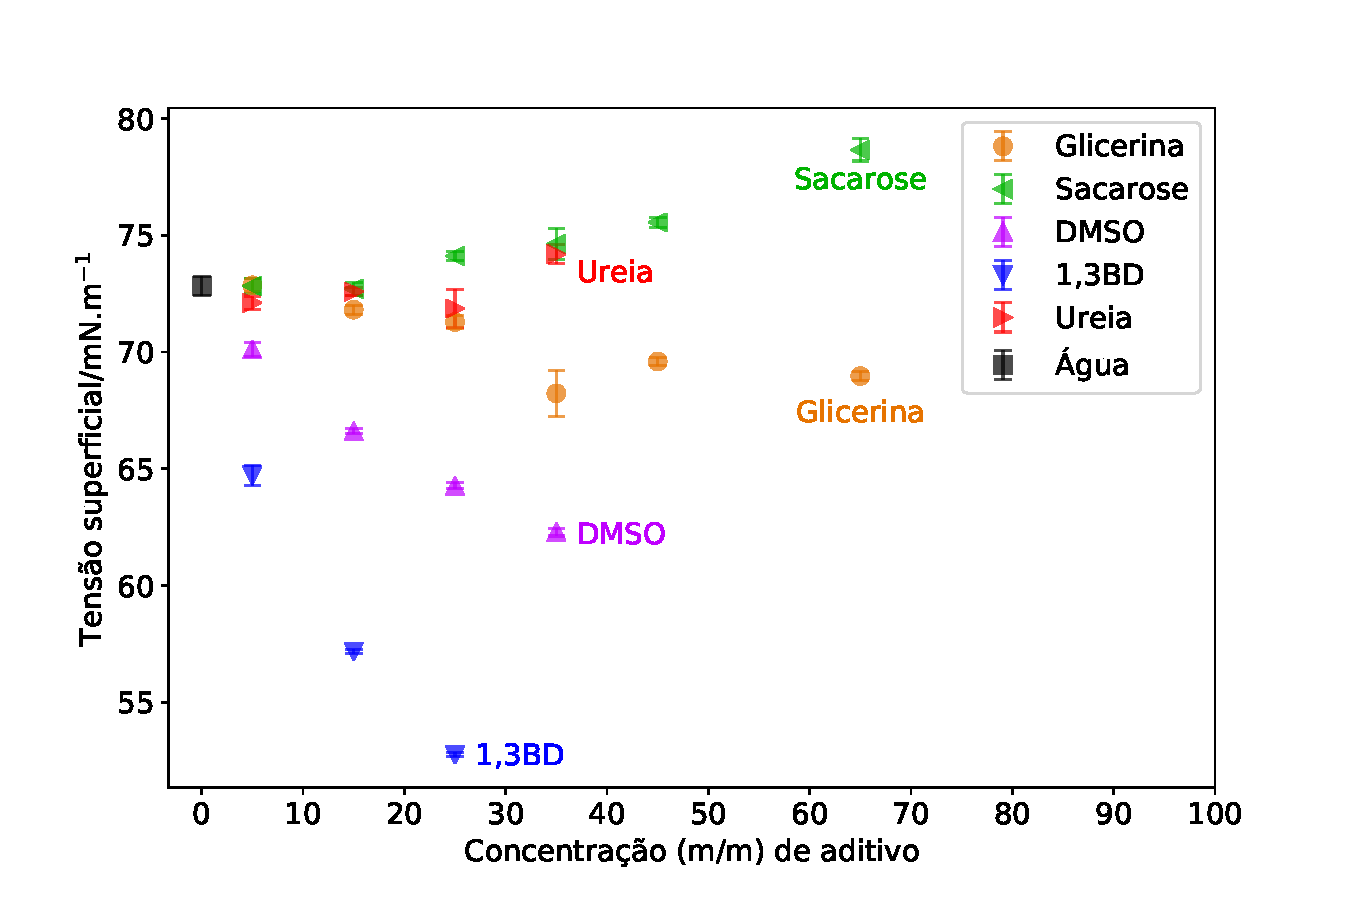
\includegraphics[width=0.7\textwidth]{imagens/propriedades/tensao_superficial}
			\caption{Tensão superficial de misturas binárias dos aditivos em água}
			\label{fig:tensao_superficial_por_conc}
		\end{figure}
		
		\begin{figure}[h]
			\centering
			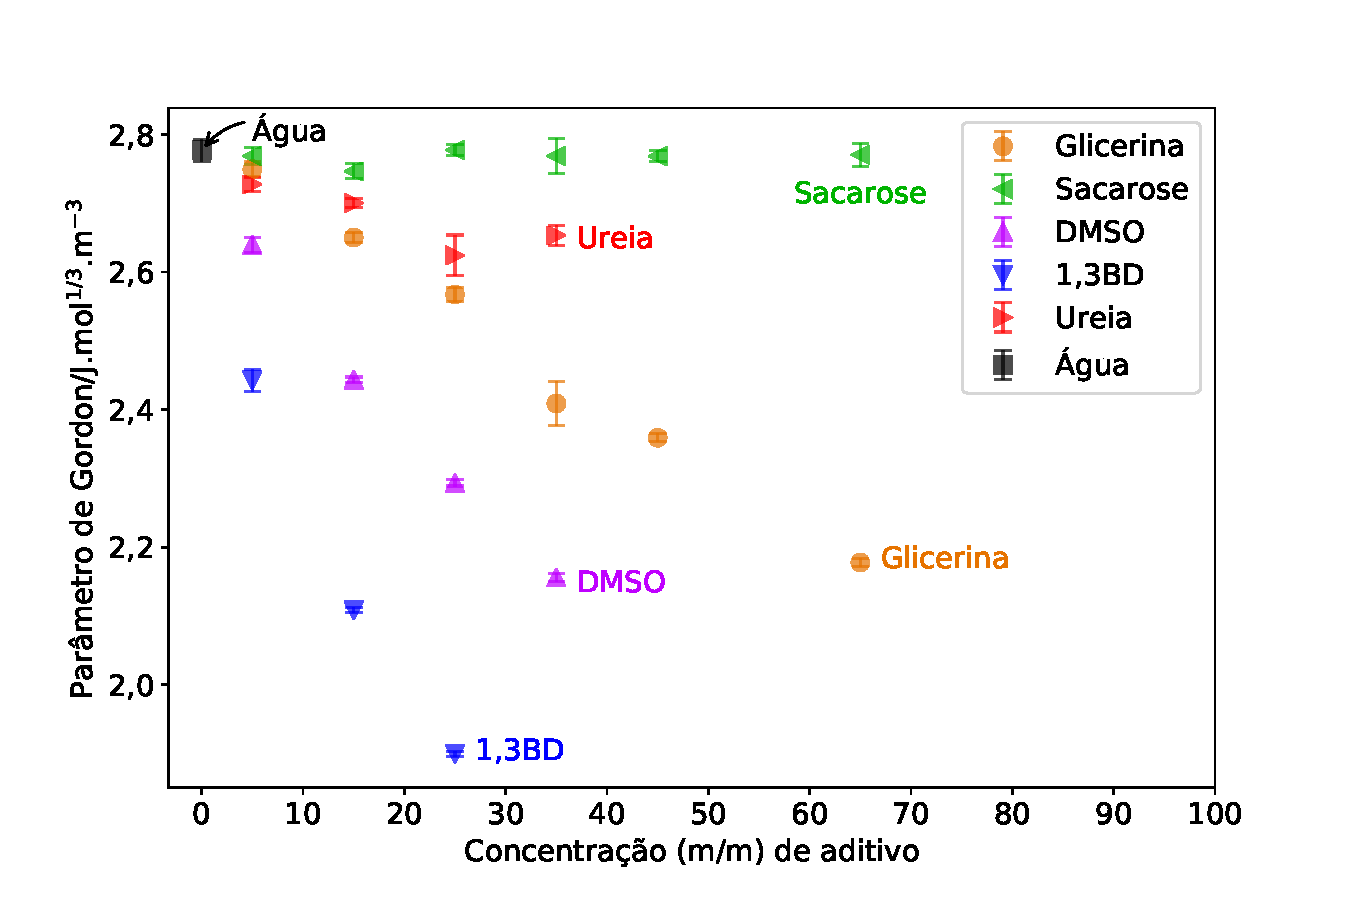
\includegraphics[width=0.7\textwidth]{imagens/propriedades/param_gordon}
			\caption{Parâmetro de Gordon das misturas binárias dos aditivos em água}
			\label{fig:param_gordon_por_conc}
		\end{figure}
		
		Podemos observar que os dois gráficos possuem basicamente o mesmo formato. A maior alteração ocorre devido à divisão pelo volume molar, onde a alta massa da sacarose mascara o aumento de sua tensão superficial, tornando os valores de \(G\) constantes. Essa divisão também diferencia as curvas de ureia e sacarose. \label{sec:correlacao_G_reologia}
		
		Pelo posição relativa das retas observadas para cada aditivo, podemos construir a seguinte correlação de estruturação do solvente:
		
		\begin{equation*}
			\textrm{1,3-BD} < \textrm{DMSO} < \textrm{Glicerina} < \textrm{Ureia} < \textrm{Sacarose}
		\end{equation*}
		
		Essa sequência possui grande correlação com o comportamento reológico (com exceção da ureia). \BD, que possui a menor estruturação, reduz mais fortemente a viscosidade das micelas. Já a sacarose praticamente não afetou a estruturação do solvente, e também não afetou muito a viscosidade. Como mencionado, a ureia é uma exceção devido à grande alteração na constante dielétrica, que deve dessorver moléculas de salicilato das micelas e aumentar sua carga. Isso faz com que o mecanismo principal de relaxação seja a reptação na faixa de concentração estudada, então a viscosidade é sempre alta.
		
		Um mecanismo possível para esse acontecimento é o seguinte. A rede criada pelo solvente é enfraquecida quando a estruturação do solvente (parâmetro de Gordon) está baixa, como está esboçado na \autoref{fig:estrutura_agua_G}. Logo, a movimentação das cadeias das micelas é favorecida, o mecanismo de reptação é acelerado, e então a viscosidade é mais baixa.
		
		\begin{figure}[h]
			\centering
			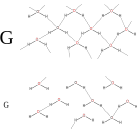
\includegraphics[width=0.5\textwidth]{imagens/Estrutura_agua_G}
			\caption{Ilustração do efeito do parâmetro de Gordon na estruturação do solvente}
			\label{fig:estrutura_agua_G}
		\end{figure}
		
		\FloatBarrier
		
		Para compreender o efeito do parâmetro de Gordon nas titulações, foram criadas figuras comparativas, da mesma maneira que nas seções anteriores. Os comparativos para a formação de micelas gigantes e micelas esféricas estão nas Figuras \ref{fig:cwlm_dhwlm_por_g} e \ref{fig:cmc_dh_por_g}, respectivamente.
		
		\begin{figure}[h]
			\begin{subfigure}[t]{0.5\textwidth}
				\centering
				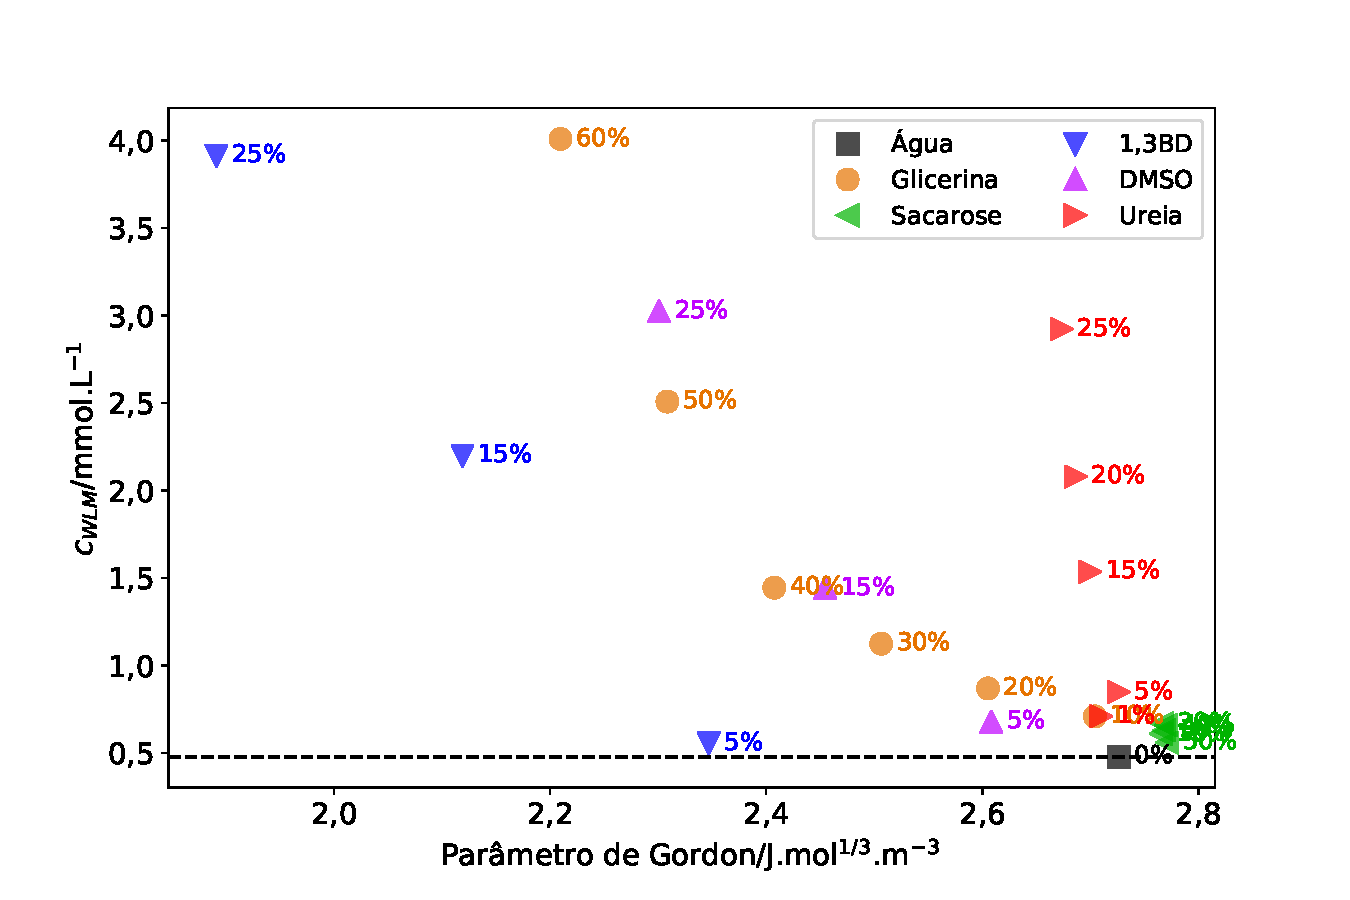
\includegraphics[width=\linewidth]{imagens/itc/Cwlm_por_G}
				\caption{\cwlm}
				\label{fig:cwlm_por_g}
			\end{subfigure} %
			\begin{subfigure}[t]{0.5\textwidth}
				\centering
				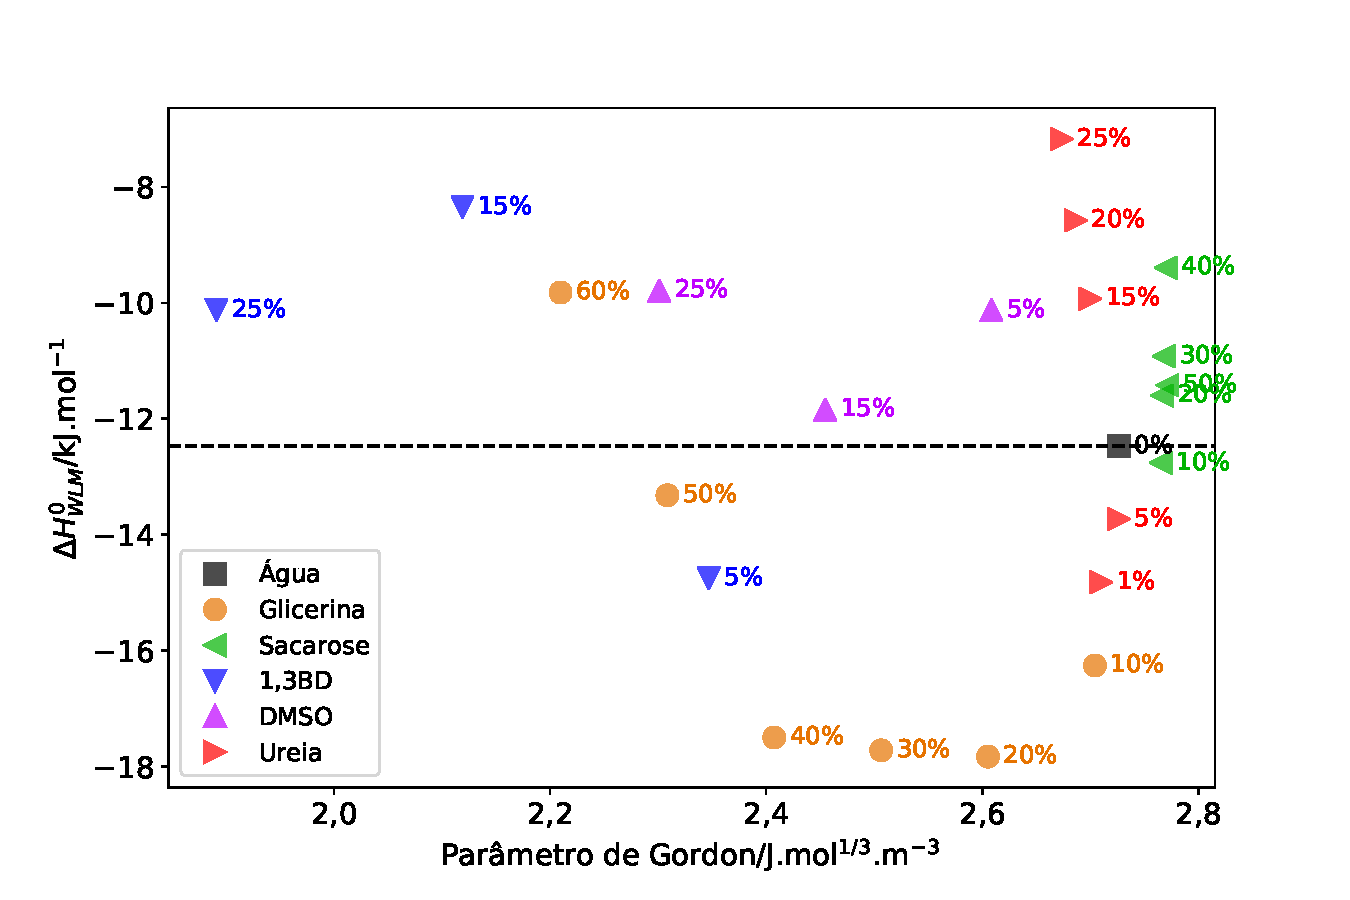
\includegraphics[width=\textwidth]{imagens/itc/DHwlm_por_G}
				\caption{\DHwlm}
				\label{fig:dhwlm_por_g}
			\end{subfigure}
			\caption{\cwlm{} e \DHwlm{} em função do parâmetro de Gordon}
			\label{fig:cwlm_dhwlm_por_g}
		\end{figure}
		
		\begin{figure}[h]
			\begin{subfigure}[t]{0.5\textwidth}
				\centering
				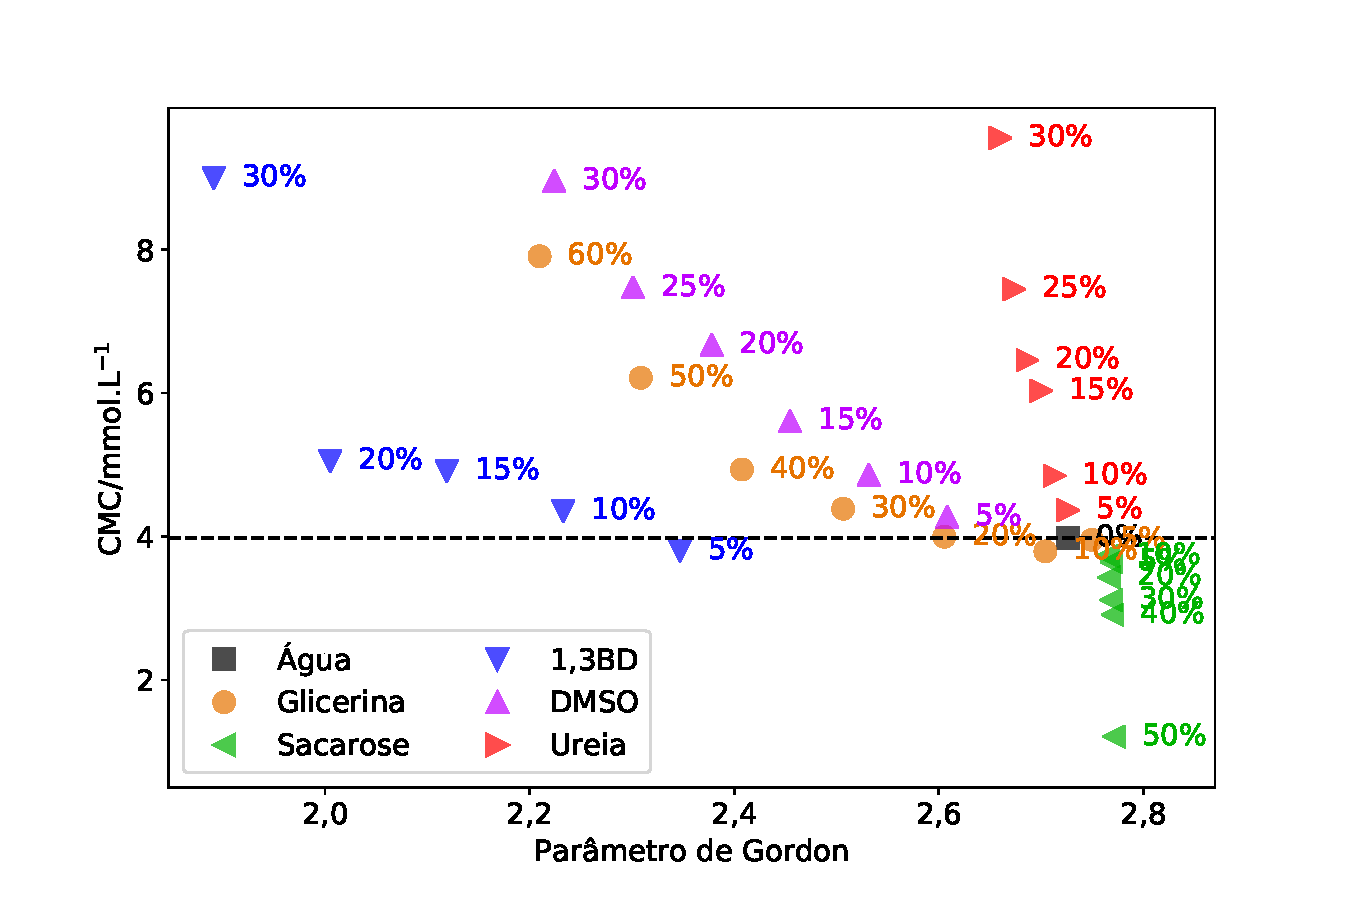
\includegraphics[width=\textwidth]{imagens/itc/CMC_por_G}
				\caption{\cmc}
				\label{fig:cmc_por_g}
			\end{subfigure} %
			\begin{subfigure}[t]{0.5\textwidth}
				\centering
				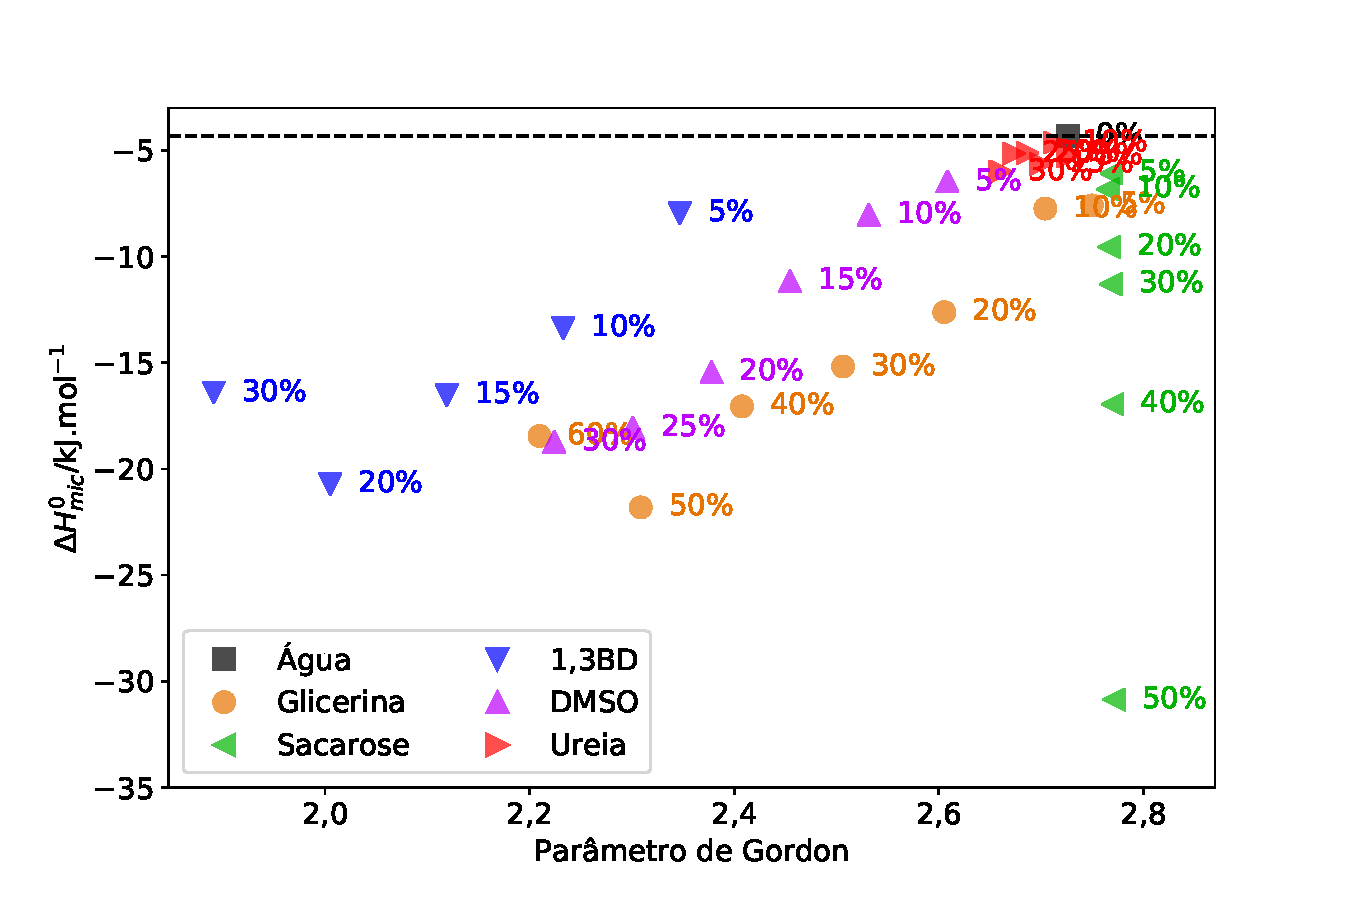
\includegraphics[width=\linewidth]{imagens/itc/DH_por_G}
				\caption{\DHmic}
				\label{fig:dh_por_g}
			\end{subfigure}
			\caption{\cmc{} e \DHmic{} em função do parâmetro de Gordon}
			\label{fig:cmc_dh_por_g}
		\end{figure}
		
		Pela inclinação das retas observadas nas Figuras \ref{fig:cwlm_por_g} e \ref{fig:cmc_por_g}, podemos observar o quão forte é o efeito de uma mudança no parâmetro de Gordon do aditivo específico na concentração de micelização. A ureia possui o efeito mais forte, onde uma pequena variação de \(G\) aumentou muito a \cmc e \cwlm, porém isso se deve principalmente ao aumento de \(\varepsilon\). Sacarose não afetou a \cwlm{} e diminuiu a \cmc, pelas razões já discutidas. Os outros três aditivos seguem uma tendência semelhante, onde uma diminuição de \(G\) resulta no aumento gradativo de \cwlm{} e \cmc. Pela inclinação, \BD{} possui o efeito mais brando na \cwlm, mas se a concentração de aditivo for levada em consideração também, vemos que seu efeito é bastante significativo, atingindo a \cwlm{} de 4 \mM{} com 25\% de aditivo, comparado com glicerina, que atingiu essa concentração com 60\%. Interessantemente, até 20\%, o efeito do \BD{} na \cmc{} é bastante pequeno, menor que o DMSO, e há um salto em 30\%, equiparando-se ao DMSO.
				
		As \DHwlm{} não possuem uma ordenação clara. Ureia aparenta ter comportamentos divergentes entre soluções de concentrações baixas (\(<\) 15\%) e altas (\(\ge\) 15\%). Já a \DHmic{} possui padrões, como os valores de ureia agrupados, pois não há salicilato para ser dessorvido. Glicerina e DMSO novamente possuem um comportamento relativamente próximo, e \BD{} tem o menor efeito na entalpia por variação de \(G\). A sacarose diminui a \DHmic{} e a \cmc{}, apesar de não afetar \(G\), indicando que seu papel está relacionado com a interação com as micelas, não somente seu efeito no solvente.
		
		A correlação do parâmetro de Gordon é especialmente forte com o comportamento reológico (página \pageref{sec:correlacao_G_reologia}), e, como será visto há algumas correlações que podem ser feitas com a calorimetria. Deve ser enfatizado que esse parâmetro, por si só, também não explica o comportamento completo. É necessário combinar todas essas considerações para entender o sistema. Por exemplo, se um aditivo for ativo na superfície, os valores de tensão superficial irão decair muito fortemente, mas não necessariamente haverá uma alteração forte na estruturação do solvente. Logo, é necessário utilizar aditivos pouco ativos em superfície, e hidrofílicos, caso seja necessário estender este estudo.
		\FloatBarrier
		
		\section{Interação dos aditivos com a superfície micelar}
		
		Uma propriedade importante que deve receber enfoque é a interação dos aditivos com a superfície micelar. Aditivos que interagem fortemente afetam muito os processos de autoassociação, como demonstra o salicilato de sódio. Efeitos semelhantes, mas menos intensos, podem complementar os parâmetros levantados até o momento.
		
		Estudos da influência de álcoois lineares na viscosidade de micelas gigantes de C\textsubscript{16}TASal e CPySal\cite{Bayer1986} mostraram que quando álcoois de cadeia curta interagiam com a superfície micelar, agem como um cossolvente e diminuem o comprimento das micelas, logo diminuindo sua viscosidade. Caso \BD{} se comporte de maneira similar, esse é mais um efeito que pode resultar nas quedas fortes da viscosidade. Um estudo mostra que o \BD{} interage como cosurfactante em cristais líquidos, o que reforça a teoria de seu efeito em micelas gigantes.\cite{Iwanaga1998a} A reologia oscilatória (\autoref{sec:reologia_oscilatoria}) mostra que o módulo no platô \(G\) para as soluções com \BD{} é menor que nos outros aditivos, reforçando a ideia de que houve uma alteração na estrutura das micelas. DMSO aparentemente se localiza na superfície micelar, logo abaixo da cabeça dos surfactantes, e altera a flexibilidade de lamelas,\cite{Notman2006} portanto é possível que o mesmo ocorra com as micelas gigantes, o DMSO iria aumentar a flexibilidade. A interação entre \Sal{} e DMSO na superfície merece mais estudos.
		
		A presença desses aditivos na superfície das micelas durante a relaxação também pode afetar a hidrofilicidade das mesmas, afetando o mecanismo de ``sticky contacts''. Isso levaria a uma diminuição na viscosidade das micelas. O \BD{} poderia se localizar na superfície micelar, aumentando sua hidrofilicidade, em comparação com as metilas do grupo trimetilamônio, levando à uma diminuição na viscosidade. A glicerina, por ser mais polar, possivelmente não se concentraria tanto na mesma região que \BD, logo seria menos eficaz em diminuir a viscosidade ou aumentar a \cmc. A posição das hidroxilas do \BD{} permite que seus grupos polares sejam expostos para uma mesma direção, já a glicerina, devido à repulsão entre as três hidroxilas próximas, não permite que todas se alinhem no mesmo plano, dificultando sua inclusão na superfície micelar.0  O DMSO pode se solubilizar na superfície micelar e interagir com os grupos metila, pois é menos polar que os outros aditivos, e isso pode resultar em uma diminuição maior na viscosidade que a glicerina, mas não tanto quanto o \BD{}. 
		
		A sacarose diminui a \cmc{} de outros surfactantes, como SDS, \CTAB{} e Brij 35, pela interação de suas hidroxilas com a superfície micelar reduzindo a repulsão, e pela estruturação do solvente. Logo, a diminuição de \(n\) e \(\varepsilon\), que deveriam aumentar a \cmc{}, são compensadas e a \cmc{} é mantida. Não há uma diminuição de \cwlm, como houve de \cmc, pois o salicilato interage mais fortemente com a superfície micelar, deslocando as hidroxilas da sacarose, logo seu efeito é principalmente na estruturação do solvente.
		
		\section{Correlações simultâneas dos parâmetros com \cmc{} e \DHmic}
		\label{sec:correlacao_params_cmc_dh}
		
		Até este momento, foram feitas correlações dos parâmetros do solvente com as propriedades calorimétricas mensuradas somente um a um, com raros casos explicados considerando-se outros parâmetros simultaneamente. Seria interessante tentar correlacionar todas essas propriedades simultaneamente, ou seja, realizar uma análise multivariada. Na literatura, existem estudos que tentam utilizar análise de fatores e regressões para classificar e estudar as propriedades de solventes na química orgânica\cite{Bohle1977,Chastrette1982, ReichardtSolvents} e também na área coloidal \cite{Moya2007a}. Esses tipos de análise, chamados de regressão linear múltipla, ou ordinária (\emph{OLS}), regressão de componentes principais \emph{PLS} e regressão dos mínimos quadrados parciais \emph{PLS} são principalmente utilizados na área da química analítica, chamada de Quimiometria.\cite{MarciaQuimiometria}
		
		Uma das necessidades para esse tipo de análise é que as variáveis sejam verdadeiramente independentes umas das outras, aditivas e relevantes ao problema em questão. Como pode ser visto pela \autoref{eqn:permissividade_e_indice_refrac}, há certa colinearidade entre o índice de refração e a constante dielétrica. O que as diferencia é fundamentalmente o efeito do solvente e suas interações.
		
		Estudos de classificação dos solventes utilizam os parâmetros já mencionados, e vários outros, como pontos de ebulição, coeficientes de partição, volume molar, constante dielétrica, índice de refração, energia de HOMO e LUMO, parâmetro \(E_T(30)\) obtidos a partir de uma sonda solvatocrômica, parâmetro de Hildebrand e momento de dipolo. Não necessariamente esses parâmetros são independentes, o que resultaria numa redução da dimensão dos dados.\cite{ReichardtSolvents}
		
		O objetivo desta seção é facilitar a interpretação dos resultados calorimétricos através dos parâmetros da solução escolhidos (\(n\), \(\varepsilon\), \(G\)), e não realizar uma descrição quimiométrica completa, nem atribuir muitos significados físicos aos coeficientes encontrados. Não serão mostrados os resultados desses ajustes para reologia (utilizando a viscosidade como variável dependente, os parâmetros e concentração de NaSal como variável dependente) e calorimetria de micelas gigantes (utilizando \cwlm{} e \DHwlm{} como variáveis dependentes e os parâmetros como variáveis dependentes) pois não foram observadas boas correlações.
		
		Inicialmente, será utilizado um método quimiométrico bastante empregado, o PLS (\emph{Partial Least Squares}), depois será utilizado um método de regressão linear múltipla, mais simples, e por último as misturas binárias serão organizadas em grupos de acordo com suas similaridades, através de um dendrograma.
		
		\subsection{PLS} \index{partial least squares@\textsl{partial least squares}}
		
		Aqui será dada uma breve descrição do método de PLS (\emph{Partial Least Squares}). Mais informações podem ser encontradas no excelente livro de \citeauthor{MarciaQuimiometria}. O PLS é baseado no método de PCR (\emph{Principal Component Regression}). No PCR, uma matriz com as informações da amostra, \textbf{X}, é decomposta em duas matrizes, uma denominada escores, \textbf{T}\textsubscript{A}, e outra matriz de pesos, \textbf{L}\textsubscript{A}, e uma matriz de resíduos \textbf{E},
		
		\begin{equation}
			\mathbf{X} = \mathbf{T}_A \mathbf{L}_A^T + \mathbf{E}
			\label{eqn:decomp_PCR}
		\end{equation}
		
		A partir da matriz de pesos, que contém a informação dos componentes principais, realiza-se um ajuste de \cite{MarciaQuimiometria}
		
		\begin{equation}
			\mathbf{y} = \mathbf{T}_A\mathbf{q} + \mathbf{e}
			\label{eqn:modelo_PCR}
		\end{equation}
		
		\noindent onde \textbf{y} é a matriz com as variáveis dependentes que se pretende ajustar, \textbf{q} é o vetor de regressão, que contém os pesos de cada componente principal para realizar o ajuste, e \textbf{e} é uma matriz de resíduos. Outra maneira de se representar essa equação é por uma maneira estendida
		
		\begin{equation}
			\mathbf{y} = q_1\mathbf{t}_1 + \cdots + q_A\mathbf{t}_A + \mathbf{e}_y
			\label{eqn:modelo_PCR_estendido}
		\end{equation}
		
		O vetor de regressão \textbf{q} pode ser estimado pelo método dos mínimos quadrados, o que resulta em
		
		\begin{equation}
			\hat{\textbf{q}} = \left(  \mathbf{T}_A^T \mathbf{T}_A  \right)^{-1}\mathbf{y}
			\label{eqn:estimativa_regress_q}
		\end{equation}

		A matriz de dados nesse caso sofre uma decomposição de valores singulares (\emph{singular value decomposition}, SVD). Porém, para a análise de PLS, uma restrição é imposta durante a decomposição da matriz de dados. Ocorre um compromisso entre a explicação da variância em \textbf{X} e a previsão da variável independente \textbf{y}, então um pouco da propriedade de interesse é colocada no cálculo das variáveis latentes. O algoritmo utilizado para isso neste trabalho foi o algoritmo de NIPALS, proposto por Wold.
		
		% todo: pensar se eu ponho as eqs 74, 80 do livro da Márcia aqui.
		Foram feitas análises de PLS  com o índice de refração, constante dielétrica e parâmetro de Gordon para tentar prever a \cmc{} e a \DHmic. Utilizou-se dois componentes (de 3) em ambos os casos, os dados foram autoescalados de modo a garantir que todas as parâmetros tenham o mesmo peso no modelo final. Logo, os valores de constante dielétrica, na faixa de 50-80, não teriam um peso 50 vezes maior do que os valores de índice de refração, que estão entre 1 e 1,5. 
		
		Utilizou-se validação cruzada com 1 elemento, e sem validação cruzada, e o vetor de previsão permaneceu igual. Essas análises foram realizadas com o software Pirouette 3.11, e comparadas com uma análise que foi feita utilizando pacote \emph{sklearn}, em Python. Esse pacote é livre, ao contrário do Pirouette, então qualquer um pode reproduzir essas análises. Os resultados foram muito próximos, então não serão mostradas as figuras resultantes de ambos os métodos, somente daqueles obtidos no Pirouette. As retas de \cmc{} e \DHmic{} medidos por \cmc{} e \DHmic{} observados estão presentes nas Figuras \ref{fig:pls_cmc_pirouette} e \ref{fig:pls_dh_pirouette}, respectivamente.
		
		\begin{figure}[h]
			\centering
			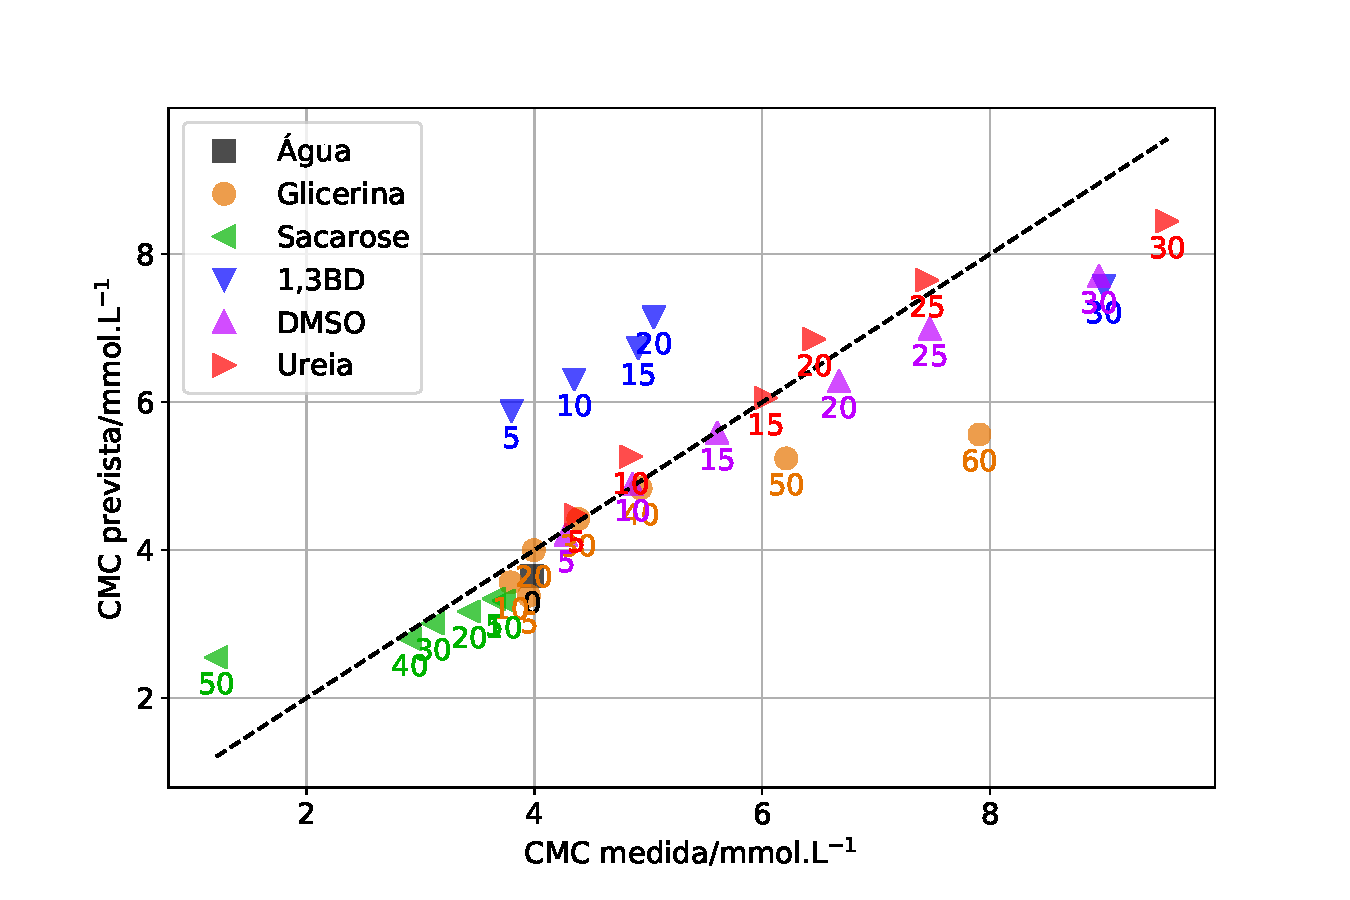
\includegraphics[width=0.7\textwidth]{imagens/itc/PLS_cmc_pirouette}
			\caption{Comportamento do modelo de \cmc{} criado por PLS, mostrando a correlação entre os valores observados e previstos. A reta preta tracejada mostra o modelo perfeito, onde há uma relação 1:1 entre o observado e o previsto. A reta vermelha mostra o modelo criado, junto com a qualidade do ajuste.}
			\label{fig:pls_cmc_pirouette}
		\end{figure}
	
		\begin{figure}[h]
			\centering
			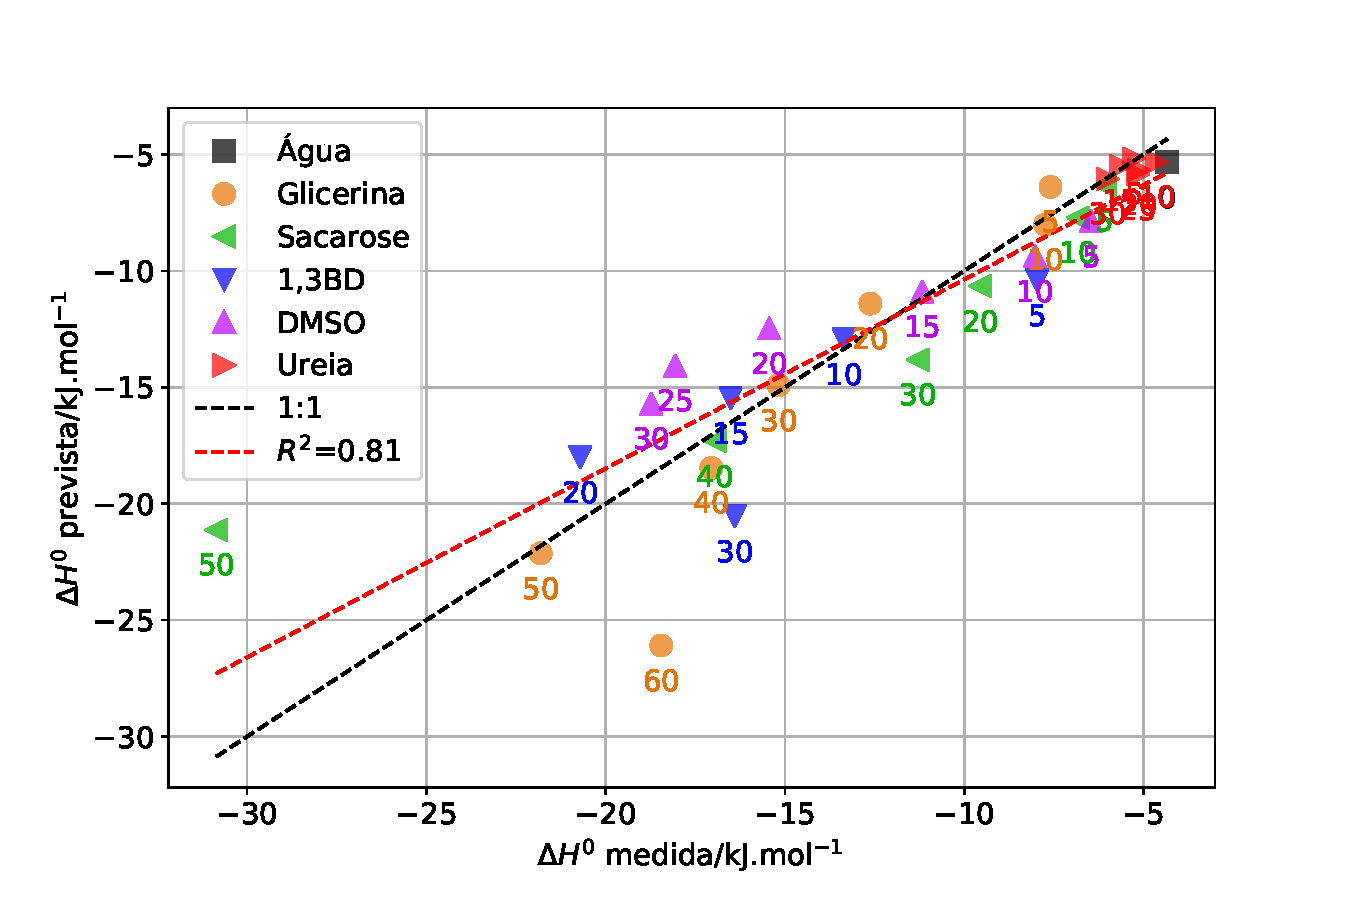
\includegraphics[width=0.7\textwidth]{imagens/itc/PLS_dh_pirouette}
			\caption{Comportamento do modelo de \DHmic{} criado por PLS, mostrando a correlação entre os valores observados e previstos. A reta preta tracejada mostra o modelo perfeito, onde há uma relação 1:1 entre o observado e o previsto. A reta vermelha mostra o modelo criado, junto com a qualidade do ajuste.}
			\label{fig:pls_dh_pirouette}
		\end{figure} 
		
		Pelas curvas de ajuste e do modelo ideal de \cmc, podemos observar que as amostras que mais divergem da região central são aquelas com alta concentração de aditivo, provavelmente porque a divergência entre suas propriedades e de água pura são muito grandes, e o processo de autoassociação é muito alterado. Além disso, observamos que todas as medidas com \BD{} estão distantes da reta 1:1, e as concentrações de 5 a 20 \% m/m estão paralelas. Isso indica que esse aditivo possui um efeito adicional, aparentemente constante nessa faixa de concentração, que resulta em valores de \cmc{} menores do que o esperado, observando somente os parâmetros escolhidos. Possivelmente, isso é consequência da tendência do \BD{} de interagir na superfície micelar, diminuir a repulsão e facilitar a autoassociação. Seria interessante realizar ajustes de \(\Delta G^\circ_\mathrm{mic}\), ao invés de \cmc, como realizaram outros estudos\cite{Abdel-Rahem2012, Moya2007a}, mas seria necessário estimar o grau de ionização das micelas (\autoref{eqn:itc_DeltaG_mic}), o que exigiria mais estudos utilizando condutividade elétrica.
		
		A previsão de \DHmic{} é melhor que de \cmc, e os compostos que mais fogem do modelo são, novamente, as soluções com maior concentração de aditivo. Em especial, temos 50\% de sacarose, 60\% de glicerina e 30\% de \BD{}.
		
		O código para fazer análise de PLS em Python, e uma figura semelhante à \autoref{fig:pls_cmc_pirouette} está na listagem \ref{lst:pls_cmc_python}.
		
		\begin{listing}[h]
			\inputminted{python}{./python/pls_cmc_sklearn.py}
			\caption{Código utilizado para gerar a dependência de \cmc{} com os parâmetros estudados, resultando na \autoref{fig:pls_cmc_pirouette}. A tabela de dados utilizada possui em cada linha as misturas utilizadas, suas concentrações em \% m/m, as variáveis dependentes (\cmc{} e \DHmic) e as variáveis independentes (\(n\), \(\varepsilon\), \(G\))}
			\label{lst:pls_cmc_python}
		\end{listing}
		
		O resultado desse modelo é um conjunto de coeficientes que, quando multiplicados pelos parâmetros escolhidos (\(n\), \(\varepsilon\), \(G\)), resultam nas propriedades (\cmc, \DHmic). Os membros do vetor não possuem unidades pois os dados foram autoescalados, então é necessário desfazer o autoescalamento para obter uma equação que utiliza coeficientes com as unidades utilizadas neste trabalho. As equações \ref{eqn:PLS_cmcs} e \ref{eqn:PLS_dhs} possuem tanto as relações em unidades usuais (a) quanto autoescaladas (b) para a \cmc{} e \DHmic, respectivamente. % (\mM, \(kJ.mol^{-1}\), \(J.mol^{-1/3}.m^{-3}\))
		
		\label{sec:PLS_micelizacao}
		
		\begin{subequations}
			\begin{align}
				\textrm{CMC}               & = -7,206G              + 0,225\varepsilon             + 27,955n            - 31,871  \label{eqn:PLS_cmc}     \\
				\textrm{CMC}_{\textrm{AS}} & = -0,941G_\textrm{AS}  + 0,864\varepsilon_\textrm{AS} + 0,319n_\textrm{AS}           \label{eqn:PLS_cmc_AS}
			\end{align}
			\label{eqn:PLS_cmcs}
		\end{subequations}
		
		\begin{subequations}
			\begin{align}
				\Delta H_\textrm{mic}^0     &= 7,64G              + 0,395\varepsilon             - 119n                + 101  \label{eqn:PLS_dh} \\
				\Delta H_\textrm{mic, AS}^0 &= 0,300G_\textrm{AS} + 0,458\varepsilon_\textrm{AS} - 0,414n_\textrm{AS}         \label{eqn:PLS_dh_AS}
			\end{align}
			\label{eqn:PLS_dhs}
		\end{subequations}
		
		Os coeficientes das equações autoescaladas estão relacionados com o quanto cada parâmetro afeta a propriedade. Em especial, os sinais mostram se um coeficiente aumenta ou diminui a propriedade modelada. Por exemplo, na \autoref{eqn:PLS_cmc_AS}, o parâmetro de Gordon possui um sinal negativo. Isso significa que um aumento de \(G\) resulta numa diminuição de \cmc, o que está de acordo com a interpretação fornecida para \(G\), que é a coesividade do solvente. Solventes mais coesos resultam em penalidades entrópicas maiores, favorecendo a micelização. A constante dielétrica, por outro lado, promove a dissociação de íons da superfície micelar, logo um aumento de \(\varepsilon\) resulta num aumento de \cmc, pois a repulsão entre os surfactantes é maior. O índice de refração, ou melhor, a diferença entre o índice de refração do meio e do surfactante, está relacionado com a atração entre as moléculas de surfactante. Quanto maior for \(n\), mais próximos são os índices de refração, menor é a atração e maior é a \cmc.
		
		A visualização do efeito desses parâmetros na \DHmic{} é menos trivial. Para interpretar esse fenômeno, é necessário entender a origem da entalpia de micelização. % todo: pesquisar e colocar aqui.
		Observamos que somente o índice de refração possui um sinal negativo, logo um aumento de \(n\) resulta numa diminuição de \DHmic{} (tornando-se mais negativo). Por outro lado, \(G\) e \(\varepsilon\) mostram que aumentos em seus valores resultam em uma diminuição na amplitude de \DHmic. 
		
		\vfill
		
		\FloatBarrier
		\subsection{OLS} \index{ordinary least squares@\textsl{ordinary least squares}}
		
		Outra metodologia que pode ser utilizada para realizar essas correlações é a dos mínimos quadrados ordinários (\emph{ordinary least squares}, OLS). Esse método é mais simples do que o PLS, pois não ocorre uma decomposição em componentes principais. Neste caso, o ajuste é feito reduzindo-se os mínimos quadrados de \cite{MarciaQuimiometria}
	
		\begin{equation}
			\mathbf{A} = \mathbf{CB} + \mathbf{E}
			\label{eqn:ols_modelo_matricial}
		\end{equation}
		
		\noindent onde \textbf{A} é a matriz de resposta \(I \times J\), neste caso, ou \cmc{} ou \DHmic, \textbf{B} é uma matriz \(L \times J\) com os coeficientes que fornecem os pesos para as variáveis, \textbf{C} é uma matriz \(I \times L\) com as variáveis independentes e \textbf{E} é uma matriz \(I \times J\) com os erros de cada ponto. \(I\) é o número de amostras estudado, \(L\) é o número de coeficientes esperado e \(J\) é o número de variáveis independentes utilizado. A nomenclatura pode ser comparada à lei de Beer, \(A = (\varepsilon b)c + \mathrm{erro}\).
		
		Para o estudo da \cmc, a \autoref{eqn:ols_modelo_cmc} pode ser reduzida para
		
		\begin{equation}
		\textrm{CMC} = a_G \cdot G + a_\varepsilon \cdot \varepsilon + a_n \cdot n + e
		\label{eqn:ols_modelo_cmc}
		\end{equation}
		
		Esse tipo de ajuste é igual ao ajuste de uma equação linear, porém com mais de uma variável independente, e é mais recomendado quando o número de variáveis independentes é pequeno.\cite{MarciaQuimiometria}
		
		Foram feitos ajustes por mínimos quadrados ordinários tanto para a previsão da \cmc{} quanto a \DHmic. Os resultados dos ajustes estão nas Figuras \ref{fig:ols_cmc_python} e \ref{fig:ols_dh_python}.
		
		\begin{figure}[h]
			\centering
			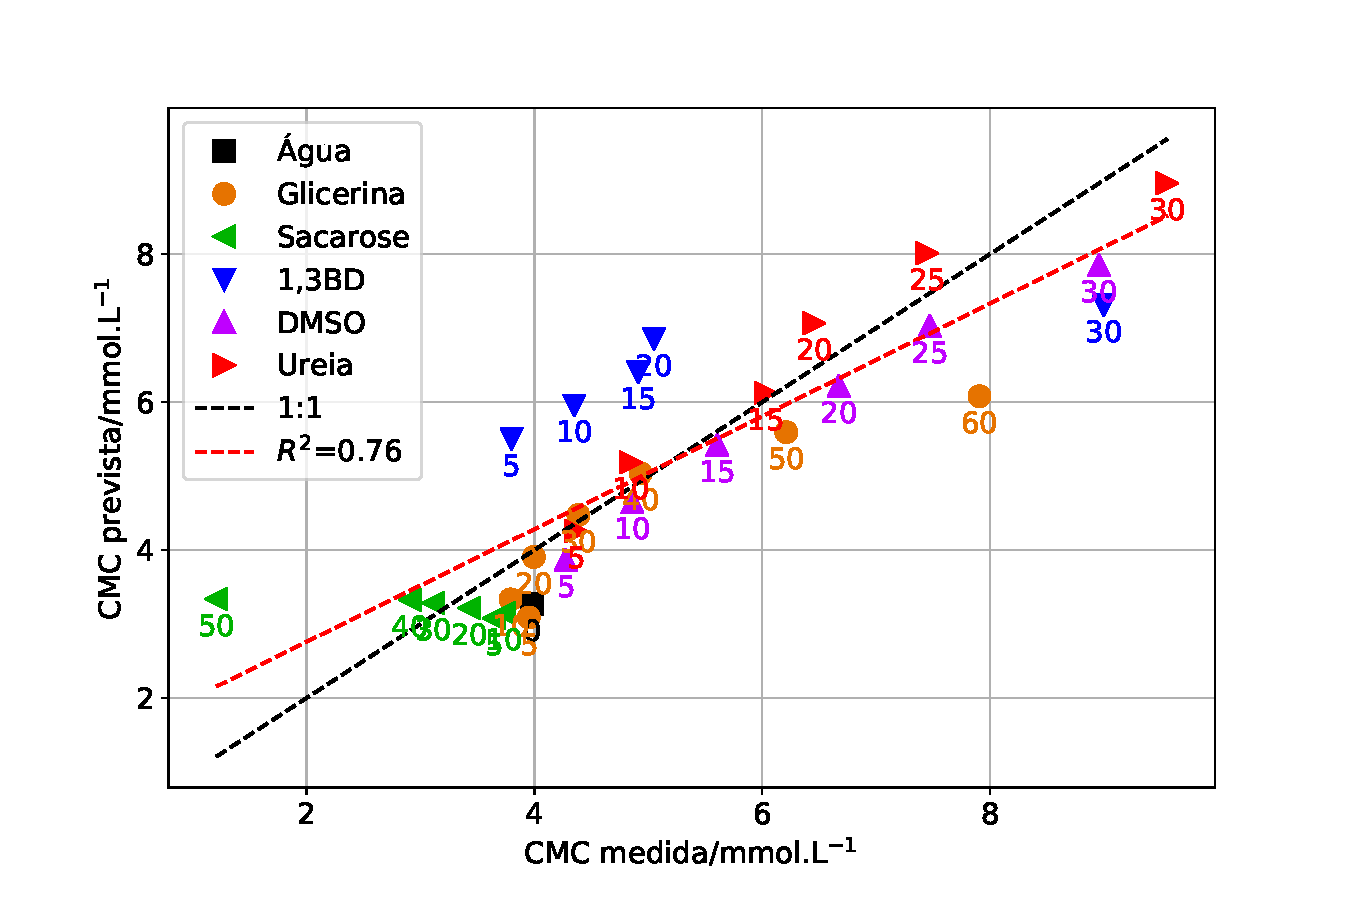
\includegraphics[width=0.7\textwidth]{imagens/itc/ols_cmc_python}
			\caption{Comportamento do modelo de \cmc{} criado por OLS, mostrando a correlação entre os valores observados e previstos. A reta preta tracejada mostra o modelo perfeito, onde há uma relação 1:1 entre o observado e o previsto. A reta vermelha mostra o modelo criado, junto com a qualidade do ajuste.}
			\label{fig:ols_cmc_python}
		\end{figure}
		
		\begin{figure}[h]
			\centering
			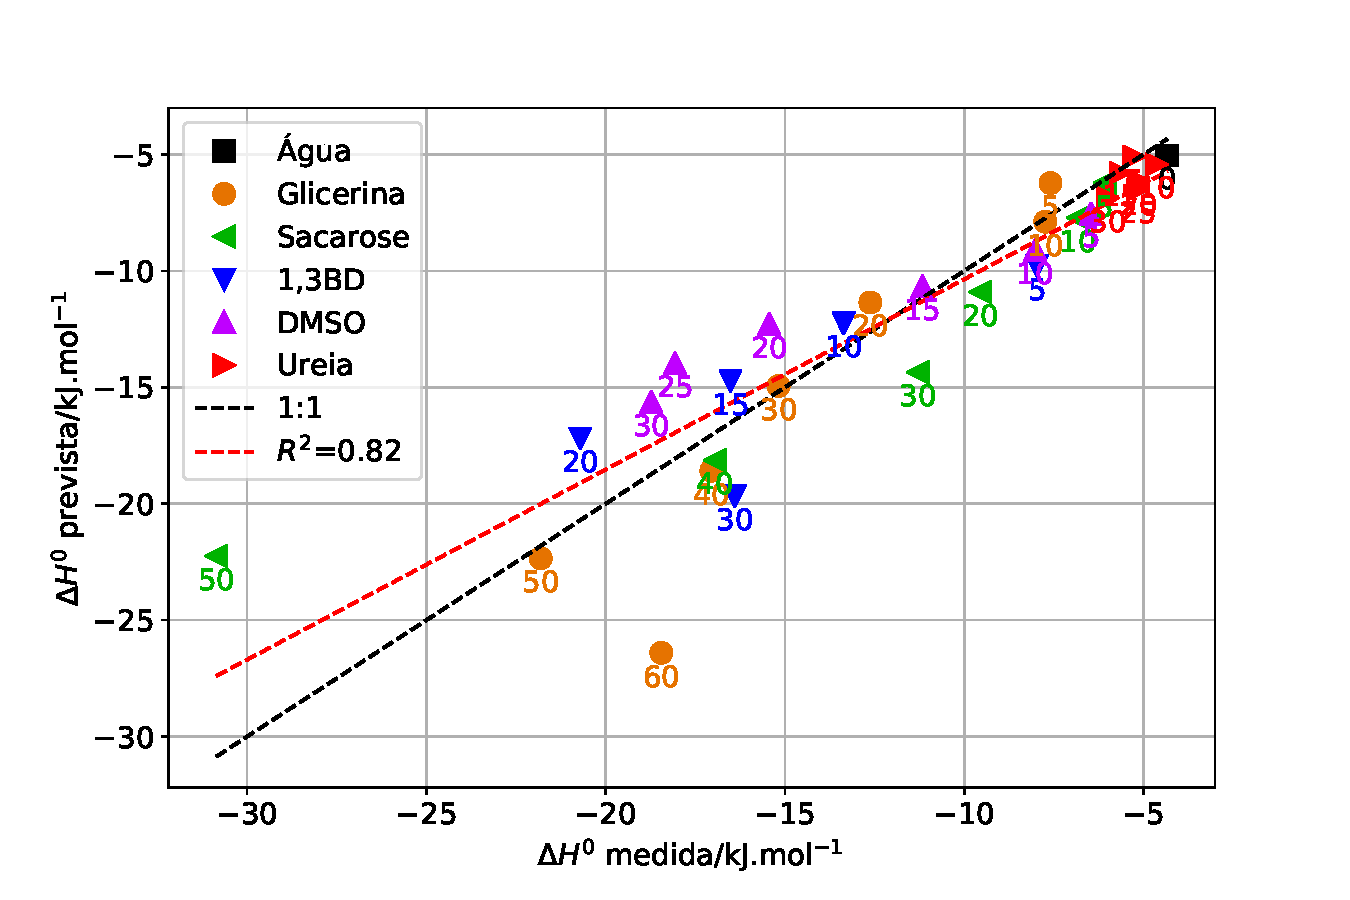
\includegraphics[width=0.7\textwidth]{imagens/itc/ols_dh_python}
			\caption{Comportamento do modelo de \DHmic{} criado por OLS, mostrando a correlação entre os valores observados e previstos. A reta preta tracejada mostra o modelo perfeito, onde há uma relação 1:1 entre o observado e o previsto. A reta vermelha mostra o modelo criado, junto com a qualidade do ajuste.}
			\label{fig:ols_dh_python}
		\end{figure}

		Para realizar as análises e criar a \autoref{fig:ols_cmc_python}, utilizou-se o código na listagem \ref{lst:ols_cmc_python}.
		
		\begin{listing}[h]
			\inputminted{python}{./python/ols_cmc_statsmodels.py}
			\caption{Código utilizado para gerar a dependência de \cmc{} com os parâmetros estudados, resultando na \autoref{fig:ols_cmc_python}. A tabela de dados utilizada possui em cada linha as misturas utilizadas, suas concentrações em \% (m/m), as variáveis dependentes (\cmc{} e \DHmic) e as variáveis independentes (\(n\), \(\varepsilon\), \(G\)).}
			\label{lst:ols_cmc_python}
		\end{listing}
		
		Os modelos obtidos estão nas Equações \ref{eqn:ols_cmcs} e \ref{eqn:ols_dhs}. O pacote fornece os parâmetros autoescalados, e para convertê-los em parâmetros nas unidades tradicionais, é necessário desescalá-los, o que pode ser feito com o código da listagem \ref{lst:ols_cmc_conversao}.
		
		\begin{subequations}
			\begin{align}
			\textrm{CMC}               & = -7{,}073G              + 0{,}239\varepsilon             + 43{,}5n              -54{,}67  \label{eqn:ols_cmc}     \\
			\textrm{CMC}_{\textrm{AS}} & = -0{,}917G_\textrm{AS}  + 0{,}919\varepsilon_\textrm{AS} +0{,}497n_\textrm{AS}          \label{eqn:ols_cmc_AS}
			\end{align}
			\label{eqn:ols_cmcs}
		\end{subequations}
		
		\begin{subequations}
			\begin{align}
			\Delta H_\textrm{mic}^0     & = 6{,}29G              + 0{,}372\varepsilon             - 138n               + 132  \label{eqn:ols_dh} \\
			\Delta H_\textrm{mic, AS}^0 & = 0{,}258G_\textrm{AS} + 0{,}432\varepsilon_\textrm{AS} - 0{,}480n_\textrm{AS}        \label{eqn:ols_dh_AS}
			\end{align}
			\label{eqn:ols_dhs}
		\end{subequations}
		
		\begin{listing}[h]
			\inputminted{python}{./python/ols_cmc_conversão.py}
			\caption{Código utilizado para transformar os parâmetros dos ajustes de autoescalados para valores habituais.}
			\label{lst:ols_cmc_conversao}
		\end{listing}
		
		Ambos os conjuntos de equações são bastante semelhantes, o que mostra que é possível realizar essas correlações tanto com o método mais complexo (PLS) quanto o método mais simples (OLS). Como o número de parâmetros utilizado é pequeno, é recomendado utilizar o método mais simples. % todo: ref livro Márcia
		
		Assim como nas Equações \ref{eqn:PLS_cmcs} e \ref{eqn:PLS_dhs}, os coeficientes dos parâmetros estão relacionados com o quanto cada parâmetro afeta os processos. Os sinais são iguais, logo as interpretações são as mesmas.
		
		Ambos os modelos apresentados possuem validade somente para os mesmos aditivos, nas faixas empregadas. Não há garantia de que esses modelos consigam prever outros aditivos, a não ser que parâmetros adicionais, mais gerais, sejam propostos.
		
		Além disso, os parâmetros escolhidos não são necessariamente independentes, ou seja, não são ortogonais. Isso diminui a qualidade dos modelos criados. Porém, o motivo principal para a criação desses modelos foi tentar interpretar o conjunto de informações simultaneamente, o que é difícil pois o conjunto de dados possui 5 dimensões. Logo, o objetivo desse estudo foi atingido.
		
		Foram feitas correlações dos parâmetros com as propriedades das micelas gigantes, porém os ajustes foram muito ruins. Isso se deve provavelmente à maior complexidade do sistema, devido à presença de NaSal, e não é possível explicar as variações considerando-se somente três parâmetros.
		
		
		\FloatBarrier
		
		\section{Visualização das semelhanças dos solventes} \index{dendrograma}
		
		Uma maneira de visualizar a similaridade das misturas binárias é utilizando um dendrograma. Esse tipo de gráfico é produzido calculando-se a distância entre pontos. Neste caso, cada ponto, representando cada mistura, está em um espaço tridimensional, de coordenadas \(n\), \(\varepsilon\) e \(G\). Inicialmente, calcula-se a distância entre os pontos, e agrupa-se os pontos que forem mais próximos, e repete-se o cálculo de distância, agora entre os grupos. O método de cálculo para a distância entre grupos varia, podendo ser feito, por exemplo, pelo vizinho mais próximo, pelo vizinho mais distante, ou pela média. \cite{MarciaQuimiometria}
		
		Dito isso, foi montado um dendrograma das misturas binárias, que está presente na \autoref{fig:dendrograma}. Do lado esquerdo do gráfico, os solventes estão sendo vistos com grande ``criteriosidade'', onde pequenas diferenças conseguem separá-los. À medida que se anda para a direita, a ``lupa'' se afasta e os solventes começam a se agrupar, até que todos os solventes são vistos como um só. A reta vertical simboliza o ponto onde a semelhança entre as misturas é de 50\%. Nessa região, os solventes podem ser separados em 6 grupos distintos, que foram coloridos.\cite{MarciaQuimiometria}
		
		\begin{figure}[h]
			\centering
			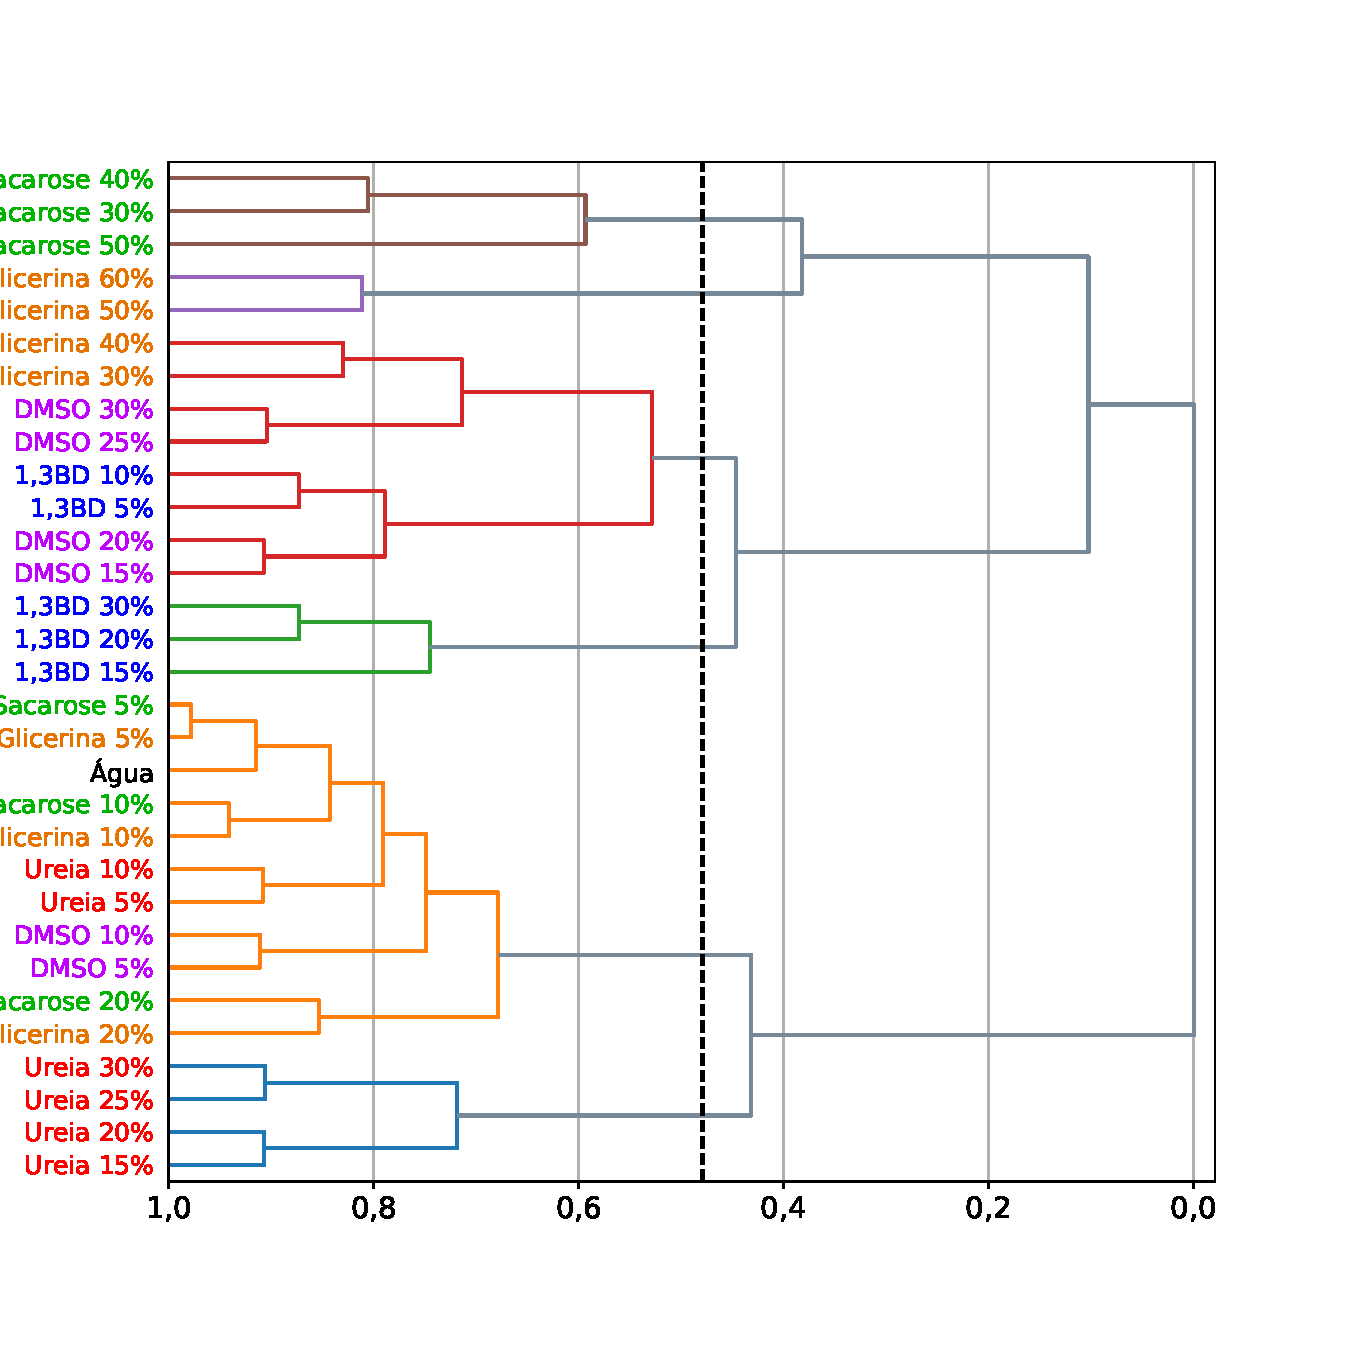
\includegraphics[width=0.7\textwidth]{imagens/propriedades/dendrograma}
			\caption{Dendrograma das propriedades das misturas binárias. A tabela de propriedades utilizada para esse gráfico é a mesma utilizada para os ajustes}
			\label{fig:dendrograma}
		\end{figure}
		
		Podemos observar a clara divisão entre dois grupos maiores. Um deles, acima, contém todas as misturas com alta concentração de aditivo, e todas as misturas de \BD{}. Abaixo, temos todas as misturas de baixa concentração de aditivo, e todas as de ureia. Dentro do grupo da alta concentração, podemos observar que a sacarose se agrupa, assim como a glicerina. Além disso, concentrações altas de glicerina se assemelham à concentrações um pouco menores de DMSO. \BD{} em baixas concentrações é parecido com DMSO em concentrações moderadas, e \BD{} em altas concentrações se isola.
		
		No grupo de baixa concentração, temos que as misturas de 5-10\% dos aditivos estão próximos, e que sacarose e glicerina 5\% são as mais próximas da água. Ureia em baixas concentrações afetou pouco as propriedades da solução, e se assemelha também à esses compostos, mais do que DMSO 5-10\%. As demais concentrações de ureia se assemelham a esse grupo, provavelmente se separando pela constante dielétrica, e se mantendo próximos pelo índice de refração e parâmetro de Gordon.
		
		Para criar esse dendrograma, utilizou-se o código da listagem \ref{lst:dendrograma}.
		
		\begin{listing}[h]
			\inputminted{python}{./python/dendrograma.py}
			\caption{Código utilizado para criar o dendrograma da \autoref{fig:dendrograma}}
			\label{lst:dendrograma}
		\end{listing}
		\FloatBarrier
		
		\section{Estimativas de \(\Delta G^\circ_{\textrm{mic}}\) e \(\Delta S^\circ_{\textrm{mic}}\)} 
		
		Através da \autoref{eqn:itc_DeltaG_mic} e \autoref{eqn:itc_gibbs_para_entropia} é possível calcular a variação energia livre de Gibbs de micelização, e a variação da entropia de micelização. Para esses cálculos, é necessário ter o grau de ionização \(\alpha\) das micelas , que deve variar muito com a composição da solução. A primeira aproximação desta seção será assumir que as micelas estão totalmente ionizadas, mas idealmente o grau de ionização deveria ser calculado através de medidas de condutividade. Além disso, as equações irão assumir que não há interação dos aditivos com as micelas, e essa será a segunda aproximação. Não existe na literatura um formalismo para a formação de micelas gigantes, então não serão calculados \(\Delta G^\circ\) e \(\Delta S^\circ\) para a formação de micelas gigantes. Os cálculos levaram em conta a concentração de aditivo para calcular a fração molar de surfactante na \cmc.
		
		Para comparações, foi criada a \autoref{fig:dg_tds_por_composto} que contém essas grandezas em função da composição dos aditivos. Ao invés de se utilizar \(\Delta S^\circ_{\textrm{mic}}\) nessa comparação, a contribuição entrópica total, \(-T\Delta S^\circ_{\textrm{mic}}\), foi utilizada. Isso permite avaliar melhor as contribuições relativas de cada grandeza, porque a faixa dos valores de \(\Delta S^\circ_{\textrm{mic}}\) é entre +60 J.mol\menosUm{} a -20 J.mol\menosUm, já os valores de \(\Delta H^\circ_{\textrm{mic}}\) estão na faixa de kJ.mol\menosUm. Essa figura também serve como uma tabela visual.
		
		\begin{figure}[h]
			\begin{subfigure}{0.5\textwidth}
				\centering
				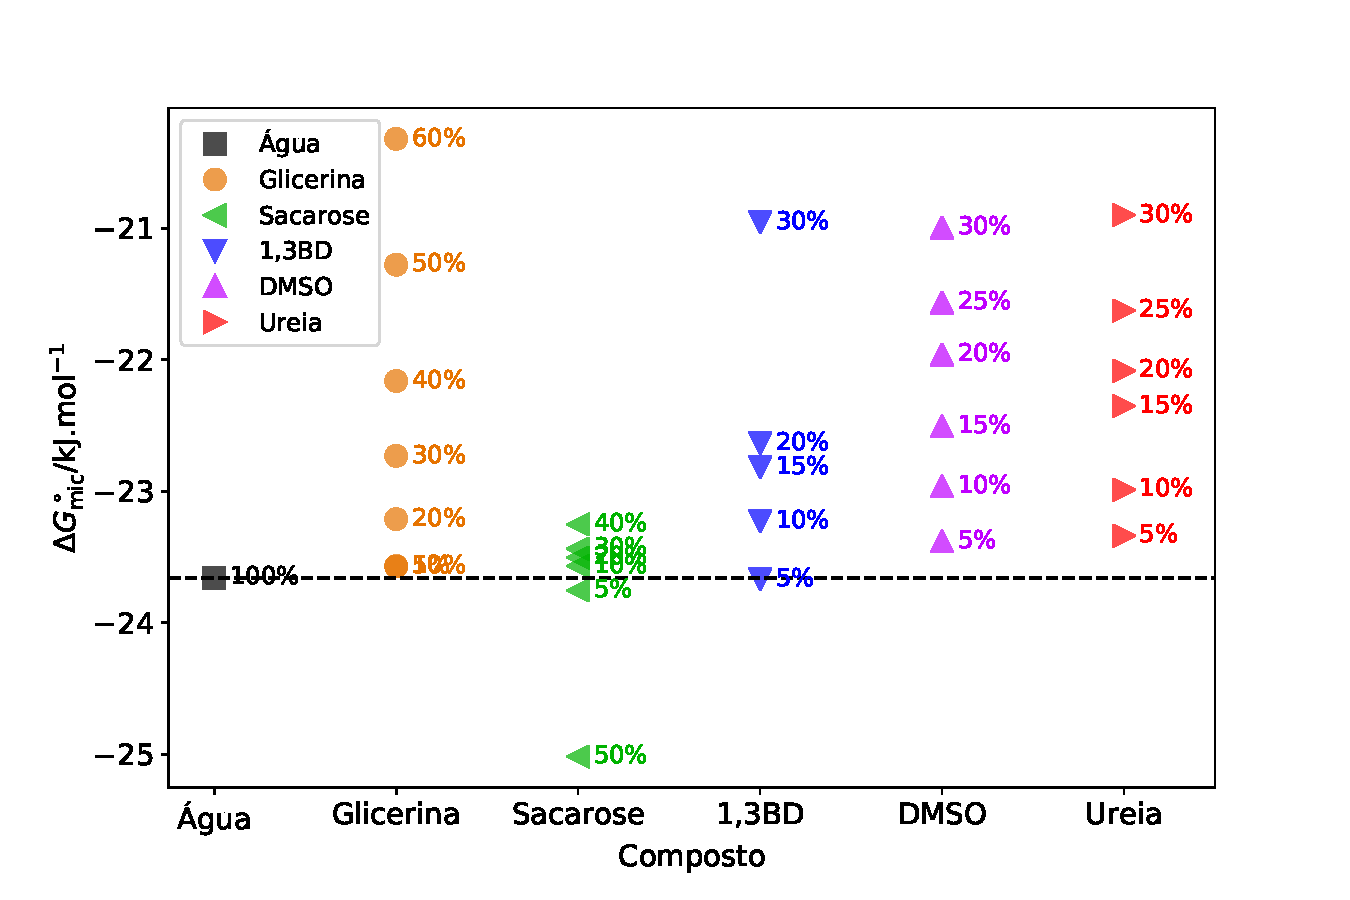
\includegraphics[width=\textwidth]{imagens/itc/DG_por_composto}
				\caption{\(\Delta G^\circ_{\textrm{mic}}\)}
				\label{fig:dg_por_composto}
			\end{subfigure}%
			\begin{subfigure}{0.5\textwidth}
				\centering
				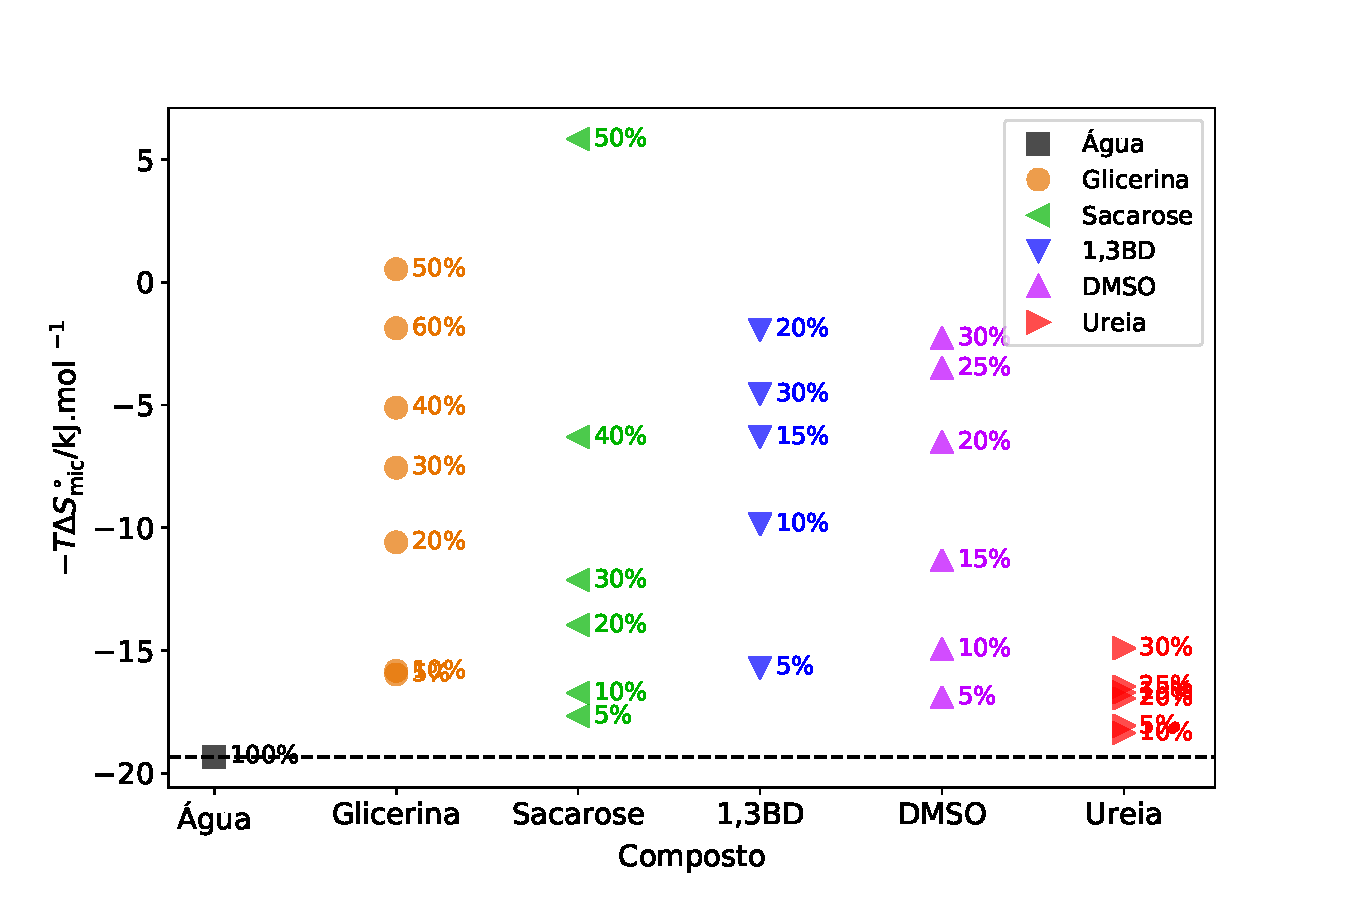
\includegraphics[width=\textwidth]{imagens/itc/TDS_por_composto}
				\caption{\(-T\Delta S^\circ_{\textrm{mic}}\)}
				\label{fig:tds_por_composto}
			\end{subfigure}
			\caption{(\ref{fig:dg_por_composto}) Energia livre de Gibbs de micelização e (\ref{fig:tds_por_composto}) contribuição entrópica para a micelização (\(-T\Delta S^\circ_{\textrm{mic}}\)) para os processos de formação de micelas de \TTAB{} em soluções dos diversos solventes binários utilizados. Essas grandezas foram calculadas a partir da \cmc{} e \DHmic. A reta horizontal é utilizada como comparação com a água.}
			\label{fig:dg_tds_por_composto}
		\end{figure}
		
		Como \(\Delta G^\circ_{\textrm{mic}}\) é obtido a partir da \cmc, é esperado que a tendência de comportamento das duas grandezas seja a mesma. De forma geral, quanto maior é a concentração de aditivo, maior é a \cmc{} e menor é a \(\Delta G^\circ_{\textrm{mic}}\). Há deslocamentos das posições de cada ponto devido à contribuição da alta concentração de aditivo no cálculo da fração molar de surfactante, como fica evidente ao se observar o comportamento da sacarose onde, apesar da \cmc{} gradualmente diminuir, os valores de \(\Delta G^\circ_{\textrm{mic}}\) oscilam ao redor do valor em água, para depois cair bruscamente em 50\%.
		
		Para todos os compostos estudados, a contribuição entrópica para a micelização se torna cada vez menor, indicando que o termo entálpico se torna mais relevante para o processo. Enquanto que, em água, o termo entrópico corresponde a aproximadamente \(\frac{4}{5}\) da contribuição total para \(\Delta G^\circ_{\textrm{mic}}\), em sacarose 50\% o termo entrópico age contra a micelização. De fato, esse é o único aditivo que levou a uma inversão no valor de \(-T\Delta S^\circ_{\textrm{mic}}\). Como esse é também o único aditivo que levou à uma diminuição de \(\Delta G^\circ_{\textrm{mic}}\), isso pode significar que a sacarose levou à micelização por sua interação com a superfície micelar, como já foi mencionado.
		
		Já os outros aditivos tiveram aumentos de \(-T\Delta S^\circ_{\textrm{mic}}\) possivelmente porque a penalidade entrópica diminui com a desestruturação do solvente. Outra observação interessante ocorre nas variações de de 50-- 60\% de glicerina e 20--30\% de \BD. Provavelmente, isso se deve à alteração significativa do solvente nessas condições, que tornou a medida em si pouco confiável, como também foi observado nas figuras anteriores. Se a tendência se mantivesse, possivelmente as concentrações mais altas de glicerina e \BD{} teriam valores de \(-T\Delta S^\circ_{\textrm{mic}}\) positivos ou próximos de zero, indicando o ponto onde a contribuição entrópica se tornou irrelevante, e a entalpia domina. Vemos também que a ureia pouco afeta o termo entálpico, mas afeta a \cmc. Porém, esse deve ser o aditivo que mais afeta a carga superficial micelar, então é difícil criar especulações confiáveis.
		
		\section{Conclusão Parcial} \index{conclusões!aditivos}
		
		Nesta parte do trabalho, mostrou-se o efeito de diversos aditivos na reologia e na calorimetria de micelas gigantes. Os experimentos reológicos mostraram como os processos de relaxação de tensão foram afetados pela adição dos aditivos, e por calorimetria observou-se a espontaneidade de formação de micelas gigantes.
		
		Todos os aditivos estudados tiveram efeitos diferentes nas micelas gigantes. Por um lado, sacarose praticamente não afetou tanto a reologia quanto a formação das micelas gigantes, apesar de promover a formação de micelas esféricas. Por outro lado, 1,3-butanodiol diminuiu fortemente a viscosidade das micelas, porém afetou a formação tanto quanto os outros aditivos. Ureia se mostrou o aditivo mais diferente de todos, aumentando a viscosidade da região de equimolaridade e diminuindo nas outras. Glicerina e DMSO tiveram efeitos semelhantes, tanto diminuindo a viscosidade das micelas quanto sua espontaneidade de formação, com DMSO tendo um efeito um pouco mais forte que glicerina.
		
		% todo: por ref
		Para explicar esses fenômenos, considerou-se alguns parâmetros. Primeiramente, o índice de refração, levantado por Hoffmann e Abdel-Rahem, constante dielétrica, levantado por Abdel-Rahem, e parâmetro de Gordon, também considerado por Abdel-Rahem, mas aplicado somente para micelas esféricas. Combinando-se esses parâmetros com efeitos mais qualitativos, como a posição dos aditivos nas micelas, foi possível explicar os fenômenos observados. O parâmetro com maior correspondência com o comportamento reológico foi o parâmetro de Gordon, relacionado à estruturação do solvente. Quanto mais próximo era o parâmetro de Gordon do solvente ao parâmetro da água pura, menos afetado era o diagrama de viscosidade. Isso pode ser consequência da diminuição da energia coesiva imposta pelo meio e, portanto, mais fácil se torna a dissipação da tensão pelas micelas gigantes. A exceção é ureia, pois é o único aditivo que aumenta a constante dielétrica do meio, e então remove espécies carregadas, como \Sal, da superfície micelar, aumentando a quantidade de \Sal{} necessária para atingir a neutralidade de carga. A interação dos aditivos com a superfície micelar deve ser considerada também, pois 1,3-butanodiol pode agir como um cosurfactante de cadeia curta, diminuindo o tempo de relaxação das micelas, diminuindo sua viscosidade.
		
		As calorimetrias de formação de micelas gigantes foram afetadas pelo solvente. Todos os solventes, com exceção de sacarose, aumentaram a concentração de formação de micelas gigantes, \cwlm, por uma combinação dos efeitos levantados. O parâmetro de Gordon diminui a penalidade entrópica do solvente, desfavorecendo agregação. O aumento da constante dielétrica aumenta a dissociação de espécies, aumentando a repulsão, também levando ao desfavorecimento da agregação. O índice de refração está relacionado à atração das moléculas de surfactante, e quanto maior for o índice, menor é a atração e menor é a tendência de formação micelar.
		
		De modo a observar o efeito de todos os parâmetros simultaneamente, foram realizados ajustes para se obter equações empíricas relacionando os parâmetros às propriedades. Foi possível correlacionar somente as concentrações micelares críticas (\cmc) e entalpias de micelização (\DHmic) aos parâmetros escolhidos. Isso ocorreu possivelmente pela maior simplicidade do sistema sem NaSal.
		
		As grandezas \(\Delta G^\circ_{\textrm{mic}}\) e \(\Delta S^\circ_{\textrm{mic}}\) foram estimadas a partir dos dados calorimétricos. Observou-se que as tendências de \(\Delta G^\circ_{\textrm{mic}}\) eram similares às de \cmc, o que é esperado. Já a \(\Delta S^\circ_{\textrm{mic}}\), ajustada para \(-T\Delta S^\circ_{\textrm{mic}}\) mostrou que quanto maior é a concentração de aditivo, menor é a contribuição entrópica para a micelização, e que em altas concentrações de sacarose, a entropia de micelização contribuía na direção oposta à micelização, apesar da \cmc{} diminuir. Isso mostra que a sacarose interage com a superfície micelar, levando à micelização, e também que os outros aditivos devem desestruturar o solvente de modo a diminuir a penalidade entrópica.
		
		Como perspectivas futuras, pode-se estudar outros aditivos para verificar o quanto os parâmetros levantados conseguem explicar outros comportamentos. Além disso, quantificar a concentração de aditivo na superfície micelar, mostrar como esses aditivos interagem com as moléculas de surfactante, com as moléculas de salicilato, e seus efeitos na cinética de quebra e recombinação micelar aprofundariam o entendimento sobre micelas gigantes. Utilizando-se condutivímetros de boa qualidade, seria possível aprofundar os estudos de calorimetria, e obter valores mais confiáveis para \(\Delta G^\circ_{\textrm{mic}}\) e \(\Delta S^\circ_{\textrm{mic}}\), o que ajudaria na discussão sobre a estruturação do solvente, penalidade entrópica e interação dos aditivos com as micelas.
		
		% todo: criar correlações agora utilizando outros parâmetros para índice de refração e cte dielétrica. Utilizar, por exemplo, (\varepsilon_r - 1 )/(2 \varepsilon_r + 1) e refração molar (V_m (n^2 - 1)/(n^2 - 2)) e cte dielétrica x dipolo, energia coesiva (raiz quadrada do param de hildebrand)
		% todo: tentar correlacionar viscosidades utilizando os parâmetros, mais a conc de salicilato como variáveis independentes
		
	\chapter{Reologia oscilatória} \index{resultados!reologia oscilatória}
	\label{sec:reologia_oscilatoria}

		Os aditivos afetam a viscosidade das soluções, como visto na \autoref{sec:efeito_aditivos_viscosidade}. Neste capítulo, será estudado o efeito dos aditivos na reologia oscilatória das micelas gigantes, que está relacionada aos processos de relaxação das micelas. Para realizar isso, foram escolhidas algumas concentrações de base, localizadas nos picos de viscosidade e no vale. Essas concentrações são 60, 100 e 260 \mM{} de NaSal. Na ausência de aditivo, também foram analisadas as concentrações de 35, 72, 189 e 365 \mM.
		
		As curvas foram ajustadas pelos modelos de Maxwell (Equações \ref{eqn:Maxwell_G1_def}, \ref{eqn:Maxwell_G2_def}), Oldroyd (Equações \ref{eqn:Maxwell_G1_def}, \ref{eqn:modelo_oldroyd_g2}), Jeffreys (Equações \ref{eqn:modelo_jeffreys_g1}, \ref{eqn:modelo_jeffreys_g2}), um modelo com dois elementos Maxwellianos, que será chamado de Dois-Modos (Equações \ref{eqn:modelo_doismodos_g1}, \ref{eqn:modelo_doismodos_g2}) e pelo recém proposto modelo de García-Saraji (Equações \ref{eqn:garcia_saraji_g1}, \ref{eqn:garcia_saraji_g2}). Dos ajustes, foram obtidos os módulos no platô, \(G\), e os tempos de relaxação \(\tau_\mathrm{rel}\), para cada dupla G' e G''. Além disso, foram calculados os coeficientes de determinação \(R^2\) (\autoref{eqn:R2}), e os coeficientes de determinação ajustado \(R\mathrm{'}^{2}\) (\autoref{eqn:R2lin}).\cite{MarciaQuimiometria} Esse tipo de estudo é utilizado na literatura para se avaliar a qualidade de um modelo.\cite{Garcia2018} Com essas informações, foram criados gráficos de Cole-Cole, onde se analisa G'' em função de G', normalizados por \(G\). Os coeficientes de determinação são dados por
		
		\begin{equation}
			R^2 = 1 - \dfrac{SQ_\mathrm{res}}{SQ_\mathrm{Tcor}}
			\label{eqn:R2}
		\end{equation} \index{coeficiente de determinação \(R^2\)}
		
		\begin{equation}
			R\mathrm{'}^{2} = 1 - \dfrac{MQ_\mathrm{res}}{MQ_\mathrm{Tcor}}
			\label{eqn:R2lin}
		\end{equation} \index{coeficiente de determinação ajustado \(R'^2\)}
		
		\noindent onde \(SQ_\mathrm{res}\) é a soma quadrática dos resíduos, \(SQ_\mathrm{Tcor}\) é a soma quadrática total corrigida, \(MQ_\mathrm{res}\) é a média quadrática dos resíduos e \(MQ_\mathrm{Tcor}\) é a média quadrática total corrigida. Esses termos estão definidos nas Equações \ref{eqn:SQres} --- \ref{eqn:MQTcor}.\cite{MarciaQuimiometria}
		
		\begin{equation}
			SQ_\mathrm{res} = \sum_{i=1}^{I} \left( y_i - \hat{y}_i \right) ^ 2
			\label{eqn:SQres}
		\end{equation}
		
		\begin{equation}
			SQ_\mathrm{Tcor} = \sum_{i=1}^{I} \left(y_i - \overline{y} \right)^2
			\label{eqn:SQTcor}
		\end{equation}
		
		\begin{equation}
			MQ_\mathrm{res} = \dfrac{SQ_\mathrm{res}}{I-p}
			\label{eqn:MQres}
		\end{equation}
		
		\begin{equation}
			MQ_\mathrm{Tcor} = \dfrac{SQ_\mathrm{Tcor}}{I - 1}
			\label{eqn:MQTcor}
		\end{equation}
		
		\noindent onde \(y_i\) é o i-ésimo ponto da curva, \(I\) é o número total de pontos, \(\hat{y}\) é a média dos valores de \(y\) (G' ou G''), \(\hat{y}_i\) é o i-ésimo valor previsto pelo modelo e \(p\) é o número de parâmetros do modelo (p.e. modelo de Maxwell possui \(G\), \(\tau_\mathrm{rel}\), \(p=2\)).
		
		O objetivo desta seção é relacionar os reogramas ao perfil de viscosidade no repouso, e determinar qual é a fonte das variações de viscosidade, e se a estrutura micelar foi afetada. Além disso, serão comparados os modelos de ajuste, e se o melhor modelo varia dependendo da região do diagrama. O coeficiente de determinação será utilizado para determinar a qualidade do ajuste, e será estudado se esse parâmetro é confiável.
		
		\section{Água}
		\label{sec:reologia_oscilatoria_experimental_agua}
		\index{resultados!reologia oscilatória!água}
		Primeiramente, será analisado a reologia oscilatória de amostras com 100 \mM{} de \CTAB{} e concentrações crescentes de NaSal. As concentrações foram escolhidas de forma a amostrar todas as regiões do diagrama de viscosidade no repouso, vide \autoref{fig:rh_agua_oscilatorio}, e mesmo assim realizar medidas com todos os aditivos. Por essa razão, as concentrações dos máximos e mínimos estão um pouco deslocadas. As concentrações utilizadas foram 35, 60, 72, 100, 189, 260 e 360 \mM{} de NaSal. Os resultados da reologia oscilatória desses pontos estão na \autoref{fig:oscilatorio_agua}.

		\begin{figure}[h]
			\centering
			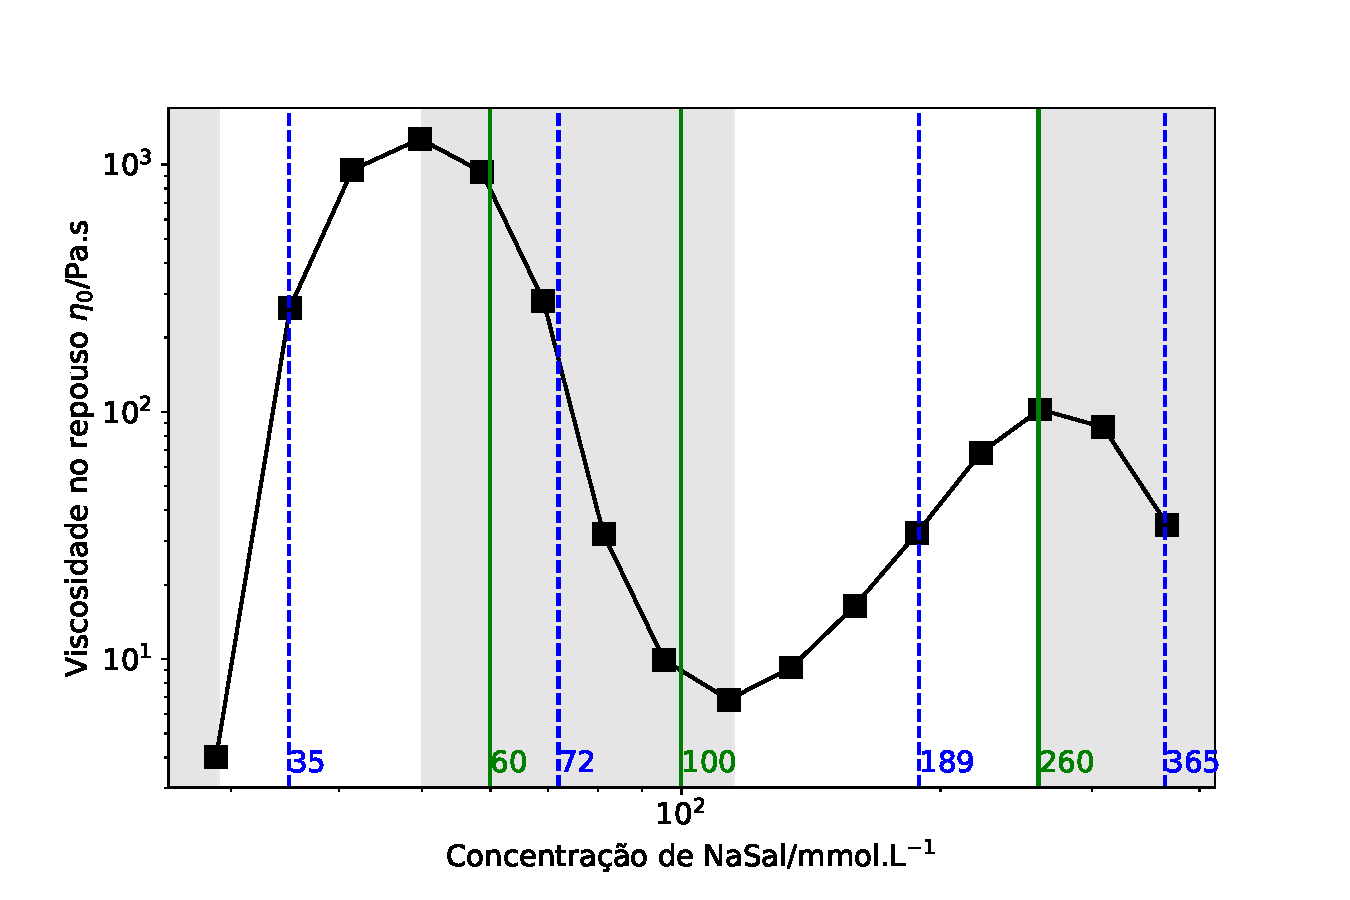
\includegraphics[width=0.7\textwidth]{imagens/reologia/RH_agua_oscilatorio}
			\caption{Perfil de viscosidade para amostras com \CTAB{} 100 \mM{} em concentrações crescentes de NaSal. As retas verdes indicam as concentrações utilizadas em todas as análises. As retas azuis tracejadas indicam as concentrações extras utilizadas na análise da água. As bandas cinzas indicam as cinco regiões desse tipo de diagrama.}
			\label{fig:rh_agua_oscilatorio}
		\end{figure}
		
		\begin{figure}[h]
			\centering
			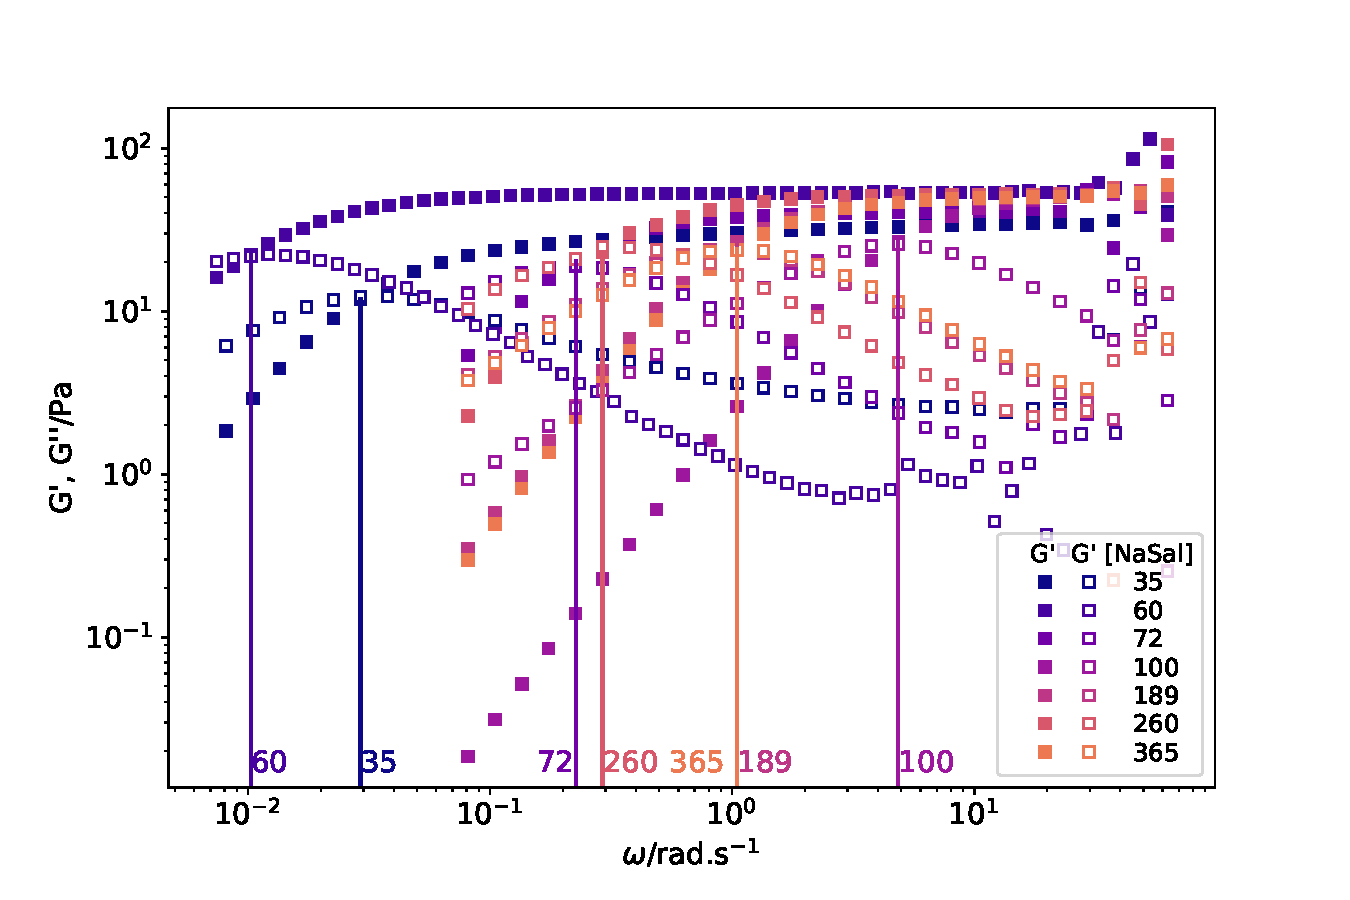
\includegraphics[width=0.7\textwidth]{imagens/reologia/oscilatorio_agua}
			%\caption[Reogramas para água]{G' (símbolos cheios) e G''(símbolos vazados) em função da frequência de perturbação \(\omega\), em rad.s\menosUm, para amostras com \CTAB{} 100\mM{} e NaSal em concentrações crescentes. Para facilitar a visualização, o ponto de cruzamento para cada curva está indicado por uma reta horizontal. As curvas de 189 e 365\mM{} de NaSal se sobrepuseram.}
			\caption{G' (símbolos cheios) e G''(símbolos vazados) em função da frequência de perturbação \(\omega\), em rad.s\menosUm, para amostras com \CTAB{} 100 \mM{} e NaSal em concentrações crescentes, em água. Para facilitar a visualização, o ponto de cruzamento para cada curva está indicado por uma reta horizontal. As curvas de 189 e 365 \mM{} de NaSal se sobrepuseram.}
			\label{fig:oscilatorio_agua}
		\end{figure}
		
		É possível ver que todas as curvas de G' atingem aproximadamente o mesmo valor em frequências altas, onde se encontra o módulo no platô, \(G\). Além disso, pode-se observar que o ponto de cruzamento, indicativo do inverso tempo de relaxação, também oscila, sendo mínimo em 60 \mM, o máximo de viscosidade, e máximo em 100 \mM, o mínimo de viscosidade. 
		
		Além disso, é possível observar que em frequências altas, os valores de G' e G'', principalmente, começam a oscilar. Essa oscilação não é real, e é devido a limitações de medida do equipamento. Para fazer os ajustes, todos os pontos a partir do momento em que começam a oscilar foram descartados. Os pontos que aparentam não seguir os modelos, mas que não mostram oscilação, foram mantidos. Os ajustes de Maxwell realizados para essas curvas estão nas Figuras \ref{fig:oscilatorio_agua_maxwell1} e \ref{fig:oscilatorio_agua_maxwell2}. O código para esse ajuste se encontra na listagem \ref{lst:ajuste_maxwell}, no fim desta seção. Os outros modelos seguiram o mesmo modelo, variando-se as equações de acordo com o modelo.
				
		\begin{figure}[h]
			\begin{subfigure}[t]{0.5\textwidth}
				\includegraphics[width=\textwidth]{imagens/reologia/oscilatorio_agua_35}
				\caption{[NaSal] = 35 \mM}
				\label{fig:oscilatorio_agua_35}
			\end{subfigure} %
			\begin{subfigure}[t]{0.5\textwidth}
				\centering
				\includegraphics[width=\textwidth]{imagens/reologia/oscilatorio_agua_60}
				\caption{[NaSal] = 60 \mM}
				\label{fig:oscilatorio_agua_60}
			\end{subfigure}
			
			\begin{subfigure}[t]{0.5\textwidth}
				\includegraphics[width=\textwidth]{imagens/reologia/oscilatorio_agua_72}
				\caption{[NaSal] = 72 \mM}
				\label{fig:oscilatorio_agua_72}
			\end{subfigure} %
			\begin{subfigure}[t]{0.5\textwidth}
				\includegraphics[width=\textwidth]{imagens/reologia/oscilatorio_agua_100}
				\caption{[NaSal] = 100 \mM}
				\label{fig:oscilatorio_agua_100}
			\end{subfigure}
		
		\caption{Ajustes de Maxwell para as curvas da \autoref{fig:oscilatorio_agua} de menor concentração de NaSal}
		\label{fig:oscilatorio_agua_maxwell1}
		\end{figure}
	
		\begin{figure}[h]
			\begin{subfigure}[t]{0.5\textwidth}
				\centering
				\includegraphics[width=\textwidth]{imagens/reologia/oscilatorio_agua_189}
				\caption{[NaSal] = 189 \mM}
				\label{fig:oscilatorio_agua_189}
			\end{subfigure} %
			\begin{subfigure}[t]{0.5\textwidth}
				\includegraphics[width=\textwidth]{imagens/reologia/oscilatorio_agua_260}
				\caption{[NaSal] = 260 \mM}
				\label{fig:oscilatorio_agua_260}
			\end{subfigure}
	
		\centering	\begin{subfigure}[t]{0.5\textwidth}
				\includegraphics[width=\textwidth]{imagens/reologia/oscilatorio_agua_365}
				\caption{[NaSal] = 365 \mM}
				\label{fig:oscilatorio_agua_365}
			\end{subfigure} 
		
			\caption{Ajustes de Maxwell para as curvas da \autoref{fig:oscilatorio_agua} de maior concentração de NaSal}
			\label{fig:oscilatorio_agua_maxwell2}
		\end{figure}
	
		Na \autoref{fig:oscilatorio_agua_35}, o ponto de cruzamento visual e o calculado divergem significantemente. Além disso, é observado um aumento de G'' em altas frequências não previsto pelo modelo, e G' também possui uma divergência da planaridade. Isso indica que não há somente um tempo de relaxação nesse sistema, e que outros modos de relaxação se tornam mais evidentes à medida que a frequência aumenta. O mesmo pode ser observado, mas em menor escala, para a \autoref{fig:oscilatorio_agua_60}.
		
		As outras amostras seguiram consideravelmente bem o modelo de Maxwell, com valores de \(R^2\) próximos à unidade, como mostram as caixas de informação. Além disso, observa-se que não há uma diferença significativa entre \(R^2\) e \(R\mathrm{'}^2\). O mesmo ocorreu para os outros modelos, então esse parâmetro não será utilizado.
		
		O mesmo procedimento foi seguido para os outros modelos. Os ajustes não serão mostrados por brevidade. Os resultados dos ajustes se encontram nas Tabelas \ref{tab:g0_agua} --- \ref{tab:R2_agua}.
		
%		\begin{table}[h]
%        \IBGEtab{%
%			\caption{Módulos no platô, \(G_0\) em Pa, em função da concentração de NaSal em \mM, de todos os ajustes}
%			\label{tab:g0_agua}
%		}%
%		{%
%			\begin{tabular}{c | c c c c c}
%				\toprule
%				NaSal & Maxwell             & OldroydB             & Jeffreys             & Dois-Modos 1            & Dois-Modos 2            \\ \midrule
%				 35   & 30,8    \(\pm\) 0,5 & 30,8     \(\pm\) 0,4 & 30,8     \(\pm\) 0,4 & 26,8        \(\pm\) 0,3 & 7,3         \(\pm\) 0,4 \\
%				 60   & 51,5    \(\pm\) 0,3 & 51,5     \(\pm\) 0,3 & 51,5     \(\pm\) 0,3 & 32          \(\pm\) 2   & 21          \(\pm\) 2   \\
%				 72   & 40,0    \(\pm\) 0,1 & 39,9     \(\pm\) 0,1 & 39,9     \(\pm\) 0,1 & 35,9        \(\pm\) 0,9 & 4,6         \(\pm\) 0,9 \\
%				 100  & 52,3    \(\pm\) 0,1 & 52,1     \(\pm\) 0,1 & 52,2     \(\pm\) 0,1 & 3,6         \(\pm\) 0,5 & 49,7        \(\pm\) 0,5 \\
%				 189  & 49,7    \(\pm\) 0,3 & 49,6     \(\pm\) 0,3 & 49,7     \(\pm\) 0,3 & 48,3        \(\pm\) 0,3 & 3,7         \(\pm\) 0,4 \\
%				 260  & 51,6    \(\pm\) 0,3 & 51,5     \(\pm\) 0,3 & 51,5     \(\pm\) 0,3 & 50          \(\pm\) 1   & 3           \(\pm\) 1   \\
%				 365  & 49,8    \(\pm\) 0,2 & 49,6     \(\pm\) 0,2 & 49,7     \(\pm\) 0,2 & 47,0        \(\pm\) 0,3 & 4,2         \(\pm\) 0,3 \\ \bottomrule
%			\end{tabular}
%		}{}
%		\end{table}  


		\begin{table}[h]
	\IBGEtab{%
		\caption{Módulos no platô \(G\), em Pa, em função da concentração de NaSal em \mM, de todos os ajustes}
		\label{tab:g0_agua}
	}%
	{%
		\begin{tabular}{c | c c c c c c}
			\toprule
			NaSal & Maxwell             & OldroydB             & Jeffreys             & Dois-Modos 1            & Dois-Modos 2            & García-Saraji      \\ \midrule
			 35   & 30,8    \(\pm\) 0,5 & 30,8     \(\pm\) 0,4 & 30,8     \(\pm\) 0,4 & 26,8        \(\pm\) 0,3 & 7,3         \(\pm\) 0,4 & 30,9  \(\pm\) 0,4  \\
			 60   & 51,5    \(\pm\) 0,3 & 51,5     \(\pm\) 0,3 & 51,5     \(\pm\) 0,3 & 32          \(\pm\) 2   & 21          \(\pm\) 2   & 51,5  \(\pm\) 0,3  \\
			 72   & 40,0    \(\pm\) 0,1 & 39,9     \(\pm\) 0,1 & 39,9     \(\pm\) 0,1 & 35,9        \(\pm\) 0,9 & 4,6         \(\pm\) 0,9 & 39,9  \(\pm\) 0,1  \\
			 100  & 52,3    \(\pm\) 0,1 & 52,1     \(\pm\) 0,1 & 52,2     \(\pm\) 0,1 & 3,6         \(\pm\) 0,5 & 49,7        \(\pm\) 0,5 & 52,31 \(\pm\) 0,09 \\
			 189  & 49,7    \(\pm\) 0,3 & 49,6     \(\pm\) 0,3 & 49,7     \(\pm\) 0,3 & 48,3        \(\pm\) 0,3 & 3,7         \(\pm\) 0,4 & 49,7  \(\pm\) 0,2  \\
			 260  & 51,6    \(\pm\) 0,3 & 51,5     \(\pm\) 0,3 & 51,5     \(\pm\) 0,3 & 50          \(\pm\) 1   & 3           \(\pm\) 1   & 51,6  \(\pm\) 0,3  \\
			 365  & 49,8    \(\pm\) 0,2 & 49,6     \(\pm\) 0,2 & 49,7     \(\pm\) 0,2 & 47,0        \(\pm\) 0,3 & 4,2         \(\pm\) 0,3 & 49,8  \(\pm\) 0,1  \\ \bottomrule
		\end{tabular}
	}{}
\end{table}   \index{resultados!reologia oscilatória!ajustes}
	
%		\begin{table}[h]
%		\IBGEtab{%
%			\caption{Tempos de relaxação, \(\tau_\mathrm{rel}\) em s, de todos os ajustes, em função da concentração de NaSal em \mM. O segundo tempo de relaxação do modelo de Jeffreys não foi incluído nesta tabela pois todos os valores eram da ordem de 1ms, e possuíam um desvio alto. Esses valores se encontram na tabela \ref{tab:outros_params_agua}.}
%			\label{tab:tr_agua}
%		}%
%		{%
%			\begin{tabular}{c | c c c c c c}
%				\toprule
%				NaSal & Maxwell               & OldroydB               & Jeffreys 1               & Dois Modos 1               & Dois Modos 2               &  \\ \midrule
%				 35   & 24      \(\pm\) 1     & 24       \(\pm\) 1     & 24        \(\pm\) 1     & 29,3        \(\pm\) 0,8   & 0,76        \(\pm\) 0,08  &  \\
%				 60   & 79      \(\pm\) 2     & 79       \(\pm\) 2     & 79        \(\pm\) 2     & 128         \(\pm\) 5     & 38          \(\pm\) 2     &  \\
%				 72   & 4,47    \(\pm\) 0,05  & 4,49     \(\pm\) 0,05  & 4,49      \(\pm\) 0,05  & 4,99        \(\pm\) 0,09  & 1,4         \(\pm\) 0,2   &  \\
%				 100  & 0,209   \(\pm\) 0,001 & 0,212    \(\pm\) 0,001 & 0,212     \(\pm\) 0,001 & 0,055       \(\pm\) 0,008 & 0,221       \(\pm\) 0,002 &  \\
%				 189  & 1,01    \(\pm\) 0,01  & 1,02     \(\pm\) 0,01  & 1,02      \(\pm\) 0,01  & 1,06        \(\pm\) 0,01  & 0,06        \(\pm\) 0,01  &  \\
%				 260  & 2,71    \(\pm\) 0,05  & 2,72     \(\pm\) 0,05  & 2,72      \(\pm\) 0,05  & 2,84        \(\pm\) 0,08  & 0,4         \(\pm\) 0,2   &  \\
%				 365  & 0,90    \(\pm\) 0,01  & 0,911    \(\pm\) 0,008 & 0,911     \(\pm\) 0,008 & 0,971       \(\pm\) 0,007 & 0,15        \(\pm\) 0,02  &  \\ \bottomrule
%			\end{tabular}
%		}{}
%	\end{table}  

		\begin{table}[h]
			\IBGEtab{%
				\caption{Tempos de relaxação, \(\tau_\mathrm{rel}\) em s, de todos os ajustes, em função da concentração de NaSal em \mM. O segundo tempo de relaxação do modelo de Jeffreys não foi incluído nesta tabela pois todos os valores eram da ordem de 1ms, e possuíam um desvio alto. Esses valores se encontram na \autoref{tab:outros_params_agua}.}
				\label{tab:tr_agua}
			}%
			{%
				\begin{tabular}{c | c c c c c c}
					\toprule
					NaSal & Maxwell               & OldroydB               & Jeffreys 1              & Dois Modos 1              & Dois Modos 2              & García-Saraji       \\ \midrule
					 35   & 24      \(\pm\) 1     & 24       \(\pm\) 1     & 24        \(\pm\) 1     & 29,3        \(\pm\) 0,8   & 0,76        \(\pm\) 0,08  & 40    \(\pm\) 8     \\
					 60   & 79      \(\pm\) 2     & 79       \(\pm\) 2     & 79        \(\pm\) 2     & 128         \(\pm\) 5     & 38          \(\pm\) 2     & 110   \(\pm\) 67    \\
					 72   & 4,47    \(\pm\) 0,05  & 4,49     \(\pm\) 0,05  & 4,49      \(\pm\) 0,05  & 4,99        \(\pm\) 0,09  & 1,4         \(\pm\) 0,2   & 4,7   \(\pm\) 0,2   \\
					 100  & 0,209   \(\pm\) 0,001 & 0,212    \(\pm\) 0,001 & 0,212     \(\pm\) 0,001 & 0,055       \(\pm\) 0,008 & 0,221       \(\pm\) 0,002 & 0,219 \(\pm\) 0,004 \\
					 189  & 1,01    \(\pm\) 0,01  & 1,02     \(\pm\) 0,01  & 1,02      \(\pm\) 0,01  & 1,06        \(\pm\) 0,01  & 0,06        \(\pm\) 0,01  & 1,04  \(\pm\) 0,03  \\
					 260  & 2,71    \(\pm\) 0,05  & 2,72     \(\pm\) 0,05  & 2,72      \(\pm\) 0,05  & 2,84        \(\pm\) 0,08  & 0,4         \(\pm\) 0,2   & 2,78  \(\pm\) 0,08  \\
					 365  & 0,90    \(\pm\) 0,01  & 0,911    \(\pm\) 0,008 & 0,911     \(\pm\) 0,008 & 0,971       \(\pm\) 0,007 & 0,15        \(\pm\) 0,02  & 0,95  \(\pm\) 0,02  \\ \bottomrule
				\end{tabular}
			}{}
		\end{table}  

%	\begin{table}[h]
%		\IBGEtab{%
%			\caption{Valores da viscosidade em altas frequências \(\eta_{\infty}\), do modelo de Oldroyd, e do segundo tempo de relaxação do modelo de Jeffreys, em ms.}
%			\label{tab:outros_params_agua}
%		}%
%		{%
%			\begin{tabular}{c | p{3cm} | p{3cm}}
%				\toprule
%				NaSal  &  \(\eta_\infty\)/Pa.s          &  \(\tau_{rel,2}\)/ms            \\ \midrule
%				35    &  0,14            \(\pm\) 0,05  &  5                \(\pm\) 1     \\
%				60    &  0,5             \(\pm\) 0,4   &  10               \(\pm\) 8     \\
%				72    &  0,07            \(\pm\) 0,02  &  1,8              \(\pm\) 0,6   \\
%				100   &  0,023           \(\pm\) 0,004 &  0,45             \(\pm\) 0,08  \\
%				189   &  0,04            \(\pm\) 0,02  &  0,7              \(\pm\) 0,3   \\
%				260   &  0,10            \(\pm\) 0,04  &  2,0              \(\pm\) 0,8   \\
%				365   &  0,07            \(\pm\) 0,01  &  1,4              \(\pm\) 0,3   \\ \bottomrule
%			\end{tabular}
%		}{} 
%	\end{table}  

	\begin{table}[h]
		\IBGEtab{%
			\caption{Valores da viscosidade em altas frequências \(\eta_{\infty}\), do modelo de Oldroyd, do segundo tempo de relaxação do modelo de Jeffreys, em ms, e dos parâmetros \(a\), em s, e b, do modelo de García-Saraji. Esses valores estão próximos aos apresentados pelos autores. \cite{Garcia2018}}
			\label{tab:outros_params_agua}
		}%
		{%
			%\begin{tabular}{c | p{3cm} | p{3cm}}
			\begin{tabular}{c | c c c c}
				\toprule
                NaSal  &  \(\eta_\infty\)/Pa.s          &  \(\tau_{rel,2}\)/ms         & \(a\)/s      &  \(b\) \\ \midrule
				35    &  0,14            \(\pm\) 0,05  &  5                \(\pm\) 1   & 2,8     0,6  &  0,3 0,1 \\
				60    &  0,5             \(\pm\) 0,4   &  10               \(\pm\) 8   & 1,6     0,8  &  0,2 0,4 \\
				72    &  0,07            \(\pm\) 0,02  &  1,8              \(\pm\) 0,6 & 0,2     0,1  &  0,6 0,2 \\
				100   &  0,023           \(\pm\) 0,004 &  0,45             \(\pm\) 0,08& 0,03    0,02 &  0,6 0,2 \\
				189   &  0,04            \(\pm\) 0,02  &  0,7              \(\pm\) 0,3 & 0,05    0,06 &  0,9 0,4 \\
				260   &  0,10            \(\pm\) 0,04  &  2,0              \(\pm\) 0,8 & 0,10    0,09 &  1,0 0,4 \\
				365   &  0,07            \(\pm\) 0,01  &  1,4              \(\pm\) 0,3 & 0,09    0,04 &  0,8 0,2 \\ \bottomrule
			\end{tabular}
		}{} 
	\end{table}  

%	\begin{table}[h]
%		\IBGEtab{%
%			\caption{Valores do coeficiente de determinação \(R^2\) de todos os ajustes. O valor de coeficiente ajustado não será incluso pois não diverge significantemente.}
%			\label{tab:R2_agua}
%		}%
%		{%
%			\begin{tabular}{c |c c c c}
%				\toprule
%				 NaSal  & Maxwell & OldroydB & Jeffreys & Dois-Modos \\ \midrule
%				35  & 0,914   & 0,925    & 0,925    & 0,988      \\
%				60  & 0,976   & 0,977    & 0,977    & 0,998      \\
%				72  & 0,997   & 0,997    & 0,997    & 0,999      \\
%				100 & 0,999   & 1,000    & 1,000    & 1,000      \\
%				189 & 0,996   & 0,997    & 0,997    & 0,999      \\
%				260 & 0,993   & 0,994    & 0,994    & 0,994      \\
%				365 & 0,998   & 0,999    & 0,999    & 1,000      \\ \bottomrule
%			\end{tabular}
%			}{}
%	\end{table}  

	\begin{table}[h]
		\IBGEtab{%
			\caption{Valores do coeficiente de determinação \(R^2\) de todos os ajustes. O valor de coeficiente ajustado não será incluso pois não diverge significantemente.}
			\label{tab:R2_agua}
		}%
		{%
			\begin{tabular}{c |c c c c c}
				\toprule
                 NaSal  & Maxwell & OldroydB & Jeffreys & Dois-Modos & García-Saraji \\ \midrule
				35  & 0,914   & 0,925    & 0,925    & 0,988  & 0.941    \\
				60  & 0,976   & 0,977    & 0,977    & 0,998  & 0.979    \\
				72  & 0,997   & 0,997    & 0,997    & 0,999  & 0.998    \\
				100 & 0,999   & 1,000    & 1,000    & 1,000  & 1.000    \\
				189 & 0,996   & 0,997    & 0,997    & 0,999  & 0.997    \\
				260 & 0,993   & 0,994    & 0,994    & 0,994  & 0.994    \\
				365 & 0,998   & 0,999    & 0,999    & 1,000  & 0.999    \\ \bottomrule
			\end{tabular}
		}{}
	\end{table}  

	Os valores de módulo no platô foram todos próximos em todos os modelos, exceto pelas primeiras concentrações, quando a rede micelar ainda está sendo formada. Isso já foi observado anteriormente\cite{Rehage1991}, e que \(G\) essencialmente não varia entre os dois picos, indicando que a estrutura micelar se mantém constante.
	
	% todo: Rehage e Hoffmann em 1991 mostraram que não muda muito entre os picos. Transição sol-gel. O módulo é dependente da concentração de partículas ou o número de pontos de crosslinking por unidade de volume. Valor constante de G0 indica que a estrutura micelar não muda em função da força iônica. No mesmo artigo, ele fala que no segundo máximo as micelas ficaram negativas.
	No modelo de Dois-Modos, não há uma restrição para os valores de \(G_{0,1}\) e \(G_{0,2}\), e observa-se que os dois módulos variam entre um valor perto de 50 Pa e outro entre 3-5 Pa, praticamente insignificante. Esse segundo módulo, provavelmente, está auxiliando no ajuste da região final de G'', onde há uma divergência para cima de G' e G''. A amostra com 60 \mM{} de NaSal, porém, mostrou dois valores bastante diferentes de \(G\) quando comparados aos outros mas, se somados, resultam no módulo dos outros modelos, mostrando que os dois elementos do modelo são, de fato, aditivos. Isso ocorreu provavelmente porque há uma região pequena antes do cruzamento, então não foi possível ajustar muito bem a curva por completo. Adquirir pontos antes do cruzamento nesse caso é, experimentalmente, muito difícil, pois exigiria muitas horas para completar uma análise, e a secagem da amostra seria difícil de ser adequadamente prevenida. Os desvios de todos os parâmetros estão semelhantes, e são maiores para as amostras longe da concentração de 100 \mM. Uma exceção é, novamente, o modelo de Dois-Modos, que possui incertezas maiores, possivelmente porque variações nesses parâmetros não resultam em mudanças significativas na qualidade do ajuste, já que utilizar um único parâmetro foi adequado.
	
	Os valores de tempo de relaxação seguem o mesmo perfil de viscosidade, como pode ser visto na \autoref{fig:oscilatorio_agua_tr}. Entre os modelos, os valores de \(\tau_{\mathrm{rel}}\) também estão todos próximos, com exceção do modelo de Dois Modos e de García-Saraji. No modelo Dois Modos, um dos tempos se aproxima dos tempos dos outros modelos, e o outro tempo é diferente. Com 60 \mM, o mesmo fenômeno ocorreu com os tempos de relaxação, mas neste caso a média dos dois tempos (128 e 38), 83, é parecido com os outros tempos de relaxação. Os tempos de relaxação para as amostras com 35 e 60 \mM{} do modelo de García-Saraji demonstraram grande variabilidade em comparação com os outros modelos, em especial a amostra com 60 \mM. Isso pode se dever à falta de pontos antes do cruzamento, sendo que o modelo necessita do perfil completo de viscosidade para estimar como o tempo de relaxação varia com a frequência. O segundo tempo de relaxação do modelo de Jeffreys, presente na \autoref{tab:outros_params_agua}, possui valores muito baixos e com incerteza alta, mostrando que esse parâmetro não é relevante ao ajuste, e também é diferente do segundo tempo de relaxação do modelo Dois-Modos. A viscosidade em frequências altas, do modelo de Oldroyd, que visa ajustar a região de alta frequência de G'', também não teve um ajuste muito bom, com altas incertezas.
	
	\begin{figure}[h]
		\centering
		\includegraphics[width=0.9\textwidth]{imagens/reologia/oscilatório_agua_tr}
		\caption{Tempos de relaxação, em segundos, calculados pelo ajuste dos quatro modelos estudados. As linhas são guias para os olhos, para mostrar a similaridade com o perfil de viscosidade (\autoref{fig:rh_agua_oscilatorio}).}
		\label{fig:oscilatorio_agua_tr}  
	\end{figure}

	
	O coeficiente de determinação possuiu valores muito altos para as amostras com concentração de NaSal maior que 100 \mM, sendo máximo nesse caso. Para as amostras com 35 e 60, o ajuste foi pior. Além disso, pode-se observar que os modelos mais complexos possuem um ajuste melhor. Isso é esperado, pois com mais parâmetros é possível aproximar mais o modelo ao dado experimental. Porém, essa melhoria pode não possuir significado físico, sendo completamente um resultado matemático. Isso ocorreu mais evidentemente nos modelos de Dois Modos e de García-Saraji, onde os parâmetros, em geral, possuíam incertezas maiores pois acabavam descrevendo as mesmas regiões dos espectros mecânicos. A \autoref{fig:ajuste_gs_tm_35} mostra os ajustes do modelo de Dois-Modos e García-Saraji para a amostra com 35 \mM{} de NaSal, evidenciando que o coeficiente de ajuste melhorado não implicou numa descrição melhor do sistema.
	
%	\begin{figure}[h]
%		\centering
%		\includegraphics[width=0.7\textwidth]{imagens/reologia/ajuste_TM_35}
%		\caption{Ajuste com o modelo de Dois-Modos do reograma completo para a amostra com 100 \mM{} de CTAB e 35 \mM{} de NaSal}
%		\label{fig:ajuste_tm_35}
%	\end{figure}

	\begin{figure}[h]
		\begin{subfigure}{0.5\textwidth}
			\centering
			\includegraphics[width=\textwidth]{imagens/reologia/ajuste_TM_35}
			\caption{Dois-Modos}
			\label{fig:ajuste_tm_35}
		\end{subfigure} %
		\begin{subfigure}{0.5\textwidth}
			\centering
			\includegraphics[width=\textwidth]{imagens/reologia/ajuste_GS_35}
			\caption{García-Saraji}
			\label{fig:ajuste_gs_35}
		\end{subfigure}
		\caption{Ajuste do reograma completo para a amostra com 100 \mM{} de \CTAB{} e 35 \mM{} de NaSal com os modelos de Dois Modos e de García-Saraji}
		\label{fig:ajuste_gs_tm_35}
	\end{figure}
	

	Utilizando os valores de \(G\) calculados pelos modelos, foi construído um diagrama de Cole-Cole, presente na \autoref{fig:colecole_agua}. Utilizou-se o \(G\) do modelo de Maxwell, já que os valores entre modelos não variaram muito. Esse tipo de diagrama possui um formato semicircular caso o conjunto de dados seguir bem o modelo de Maxwell. Essa é uma maneira alternativa de se visualizar o quão bons são os ajustes. É possível criar um diagrama sem normalizar G' e G'' por \(G\), mas isso torna a comparação entre sistemas diferentes mais difícil.

		\begin{figure}[b]
			\centering
			\includegraphics[width=0.7\textwidth]{imagens/reologia/colecole_agua}
			\caption{Diagrama de Cole-Cole com G' e G'' normalizado, para amostras com 100 \mM{} de \CTAB{} e concentrações crescentes de NaSal. A linha tracejada mostra como seria o comportamento ideal, 100\% Maxwelliano. As marcas \texttt{x} indicam o último ponto considerado nos ajustes.}
			\label{fig:colecole_agua}
		\end{figure} \index{resultados!reologia oscilatória!Cole-Cole}

	Com o diagrama de Cole-Cole, é possível observar, graficamente, que as amostras com 35 e 60 \mM{} de NaSal são as que menos se ajustam ao modelo, já as outras são melhores. É possível, a partir de diagramas como esses, estimar outras propriedades das micelas (\autoref{eqn:mesh_contorno_por_reologia}) mas isso necessita de valores confiáveis para altas frequências (à direita no diagrama), o que não ocorreu.
	
	\begin{listing}[h]
		\inputminted{python}{./python/ajuste_maxwell.py}
		\caption{Código utilizado para realizar o ajuste de Maxwell de ambos os conjuntos de dados (G' e G'') simultaneamente.}
		\label{lst:ajuste_maxwell}
	\end{listing}
	
	\FloatBarrier
	
	\section{Aditivos} \index{resultados!reologia oscilatória!aditivos}

	O mesmo processo de análise foi feito com os aditivos. Os reogramas foram divididos em várias imagens para facilitar as comparações. As misturas analisadas e as imagens são: 30 e 60\% (m/m) de Glicerina (\autoref{fig:oscilatorio_glicerina}), 50\% (m/m) de Sacarose (\autoref{fig:oscilatorio_ur_sacarose}), e 5 ( \autoref{fig:oscilatorio_ur_sacarose}), 15 e 30\% (m/m) de Ureia (\autoref{fig:oscilatorio_ur}) 15 e 25\% (m/m) de DMSO (\autoref{fig:oscilatorio_dmso}), 15 e 25\% (m/m) de \BD{} (\autoref{fig:oscilatorio_13bd}). As linhas verticais são ajudas para diferenciar as curvas, e apontam para o ponto de cruzamento.
	
	\begin{figure}[h]
		\begin{subfigure}[t]{0.5\textwidth}
			\centering
			\includegraphics[width=\textwidth]{imagens/reologia/oscilatorio_glic30p}
			\caption{Glicerina 30\%}
			\label{fig:oscilatorio_glic_30p}
		\end{subfigure} %
		\begin{subfigure}[t]{0.5\textwidth}
			\centering
			\includegraphics[width=\textwidth]{imagens/reologia/oscilatorio_glic60p}
			\caption{Glicerina 60\%}
			\label{fig:oscilatorio_glic_60p}
		\end{subfigure} %
	\caption{G' (símbolos cheios) e G'' (símbolos vazados) em função da frequência de perturbação \(\omega\), para amostras de \CTAB{} 100 \mM{}, NaSal 60, 100 e 260 \mM{} e glicerina 30 e 60\% (m/m).}
	\label{fig:oscilatorio_glicerina}
	\end{figure} 	\index{resultados!glicerina}

	\begin{figure}[h]
		\begin{subfigure}[t]{0.5\textwidth}
			\centering
			\includegraphics[width=\textwidth]{imagens/reologia/oscilatorio_sac50p}
			\caption{Sacarose 50\%}
			\label{fig:oscilatorio_sac_50p}
		\end{subfigure} %
		\begin{subfigure}[t]{0.5\textwidth}
			\centering
			\includegraphics[width=\textwidth]{imagens/reologia/oscilatorio_ur5p}
			\caption{Ureia 5\%}
			\label{fig:oscilatorio_ur_5p}
		\end{subfigure} 
	\caption{G' (símbolos cheios) e G'' (símbolos vazados) em função da frequência de perturbação \(\omega\), para amostras de \CTAB{} 100 \mM{}, NaSal 60, 100 e 260 \mM{} e sacarose 50 \% (\ref{fig:oscilatorio_sac_50p}) e ureia 5\% (m/m) (\ref{fig:oscilatorio_ur_5p})}
	\label{fig:oscilatorio_ur_sacarose}
	\end{figure} 	\index{resultados!ureia} 	\index{resultados!sacarose}

	\begin{figure}[h]
	\begin{subfigure}[t]{0.5\textwidth}
		\centering
		\includegraphics[width=\textwidth]{imagens/reologia/oscilatorio_ur15p}
		\caption{Ureia 15\%}
		\label{fig:oscilatorio_ur_15p}
	\end{subfigure} %
	\begin{subfigure}[t]{0.5\textwidth}
		\centering
		\includegraphics[width=\textwidth]{imagens/reologia/oscilatorio_ur30p}
		\caption{Ureia 30\%}
		\label{fig:oscilatorio_ur_30p}
	\end{subfigure} %
	\caption{G' (símbolos cheios) e G'' (símbolos vazados) em função da frequência de perturbação \(\omega\), para amostras de \CTAB{} 100 \mM{}, NaSal 60, 100 e 260 \mM{} e ureia 15\% e 30\% m/m}
	\label{fig:oscilatorio_ur}
	\end{figure} 	\index{resultados!ureia}

	\begin{figure}[h]
		\begin{subfigure}[t]{0.5\textwidth}
			\centering
			\includegraphics[width=\textwidth]{imagens/reologia/oscilatorio_dmso15p}
			\caption{DMSO 15\%}
			\label{fig:oscilatorio_dmso_15p}
		\end{subfigure} %
		\begin{subfigure}[t]{0.5\textwidth}
			\centering
			\includegraphics[width=\textwidth]{imagens/reologia/oscilatorio_dmso25p}
			\caption{DMSO 25\%}
			\label{fig:oscilatorio_dmso_25p}
		\end{subfigure} %
		\caption{G' (símbolos cheios) e G'' (símbolos vazados) em função da frequência de perturbação \(\omega\), para amostras de \CTAB{} 100 \mM{}, NaSal 60, 100 e 260 \mM{} e DMSO 15\% e 25\% m/m}
		\label{fig:oscilatorio_dmso}
	\end{figure} 	\index{resultados!dimetilsulfóxido}
	
	\begin{figure}[h]
		\begin{subfigure}[t]{0.5\textwidth}
			\centering
			\includegraphics[width=\textwidth]{imagens/reologia/oscilatorio_13bd15p}
			\caption{\BD{} 15\%}
			\label{fig:oscilatorio_13bd_15p}
		\end{subfigure} %
		\begin{subfigure}[t]{0.5\textwidth}
			\centering
			\includegraphics[width=\textwidth]{imagens/reologia/oscilatorio_13bd25p}
			\caption{\BD{} 15\%}
			\label{fig:oscilatorio_13bd_25p}
		\end{subfigure} %
		\caption{G' (símbolos cheios) e G'' (símbolos vazados) em função da frequência de perturbação \(\omega\), para amostras de \CTAB{} 100 \mM{}, NaSal e 1,3-butanodiol 15\% e 25\% m/m. Nem todas as amostras possuíam consistência suficiente para serem medidas no reômetro, então foram descartadas da análise.}
		\label{fig:oscilatorio_13bd}
	\end{figure} 	\index{resultados!1,3-butanodiol}

	De início, é possível observar que várias das amostras não possuem um comportamento próximo ao Maxwelliano, em especial as amostras com \BD{}, 60\% de glicerina e 30\% de ureia com 60 \mM{} de NaSal. Em comum, essas amostras possuem baixa viscosidade. Interessantemente, todas as amostras, com exceção de  \BD{} 25\%, aparentam possuir valores de \(G\) próximos, da ordem de 10-50 Pa, independente da viscosidade total da solução, o que mostra que a estrutura micelar nesses sistemas foi mantido, e a viscosidade foi afetada por mudanças no tempo de relaxação, primariamente. Além disso, as amostras com 50\% de sacarose foram as únicas analisadas que possuem a região de alta frequência de G'' bem definida, possivelmente devido à alta viscosidade do solvente.
	
	Com esses dados, foram realizados ajustes com os quatro modelos. Os coeficientes de determinação \(R^2\) se encontram na \autoref{tab:R2_aditivos}, os módulos no platô se encontram na \autoref{tab:g0_aditivos} e os tempos de relaxação se encontram na \autoref{tab:tr_aditivos}. 


%	\begin{table}[h]
%		\IBGEtab{%
%			\caption{Valores do coeficiente de determinação \(R^2\) para os ajustes das amostras com CTAB 100 \mM{}, concentrações crescentes de NaSal, também em \mM, e seletas concentrações de aditivo, em \% m/m. O valor de coeficiente ajustado não será incluso pois não diverge significativamente.}
%			\label{tab:R2_aditivos}
%		}%
%		{%
%			\begin{tabular}{c c c | c c c c}
%				\toprule
%				 Aditivo  & \% Adit & [NaSal] & Maxwell & OldroydB & Jeffreys & Dois Modos \\ \midrule
%				Glicerina & 30        & 60         & 0,981   & 0,988    & 0,988    & 0,997      \\
%				Glicerina & 30        & 100        & 0,998   & 0,999    & 0,999    & 1,000      \\
%				Glicerina & 30        & 260        & 0,998   & 0,999    & 0,999    & 1,000      \\
%				Glicerina & 60        & 60         & 0,901   & 0,941    & 0,901    & 0,912      \\
%				Glicerina & 60        & 100        & 0,991   & 0,999    & 0,999    & 1,000      \\
%				Glicerina & 60        & 260        & 0,998   & 0,999    & 0,999    & 0,999      \\
%				Sacarose  & 50        & 60         & 0,916   & 0,954    & 0,954    & 0,953      \\
%				Sacarose  & 50        & 100        & 0,992   & 0,999    & 0,999    & 1,000      \\
%				Sacarose  & 50        & 260        & 0,951   & 0,989    & 0,989    & 0,998      \\ \midrule
%				  Ureia   & 5         & 60         & 0,989   & 0,990    & 0,990    & 0,999      \\
%				  Ureia   & 5         & 100        & 0,999   & 0,999    & 0,999    & 1,000      \\
%				  Ureia   & 5         & 260        & 0,998   & 0,999    & 0,999    & 0,999      \\
%				  Ureia   & 15        & 60         & 0,913   & 0,928    & 0,928    & 0,969      \\
%				  Ureia   & 15        & 100        & 0,998   & 0,999    & 0,999    & 1,000      \\
%				  Ureia   & 15        & 260        & 0,997   & 0,998    & 0,998    & 0,999      \\
%				  Ureia   & 30        & 60         & 0,765   & 0,786    & 0,786    & 0,938      \\
%				  Ureia   & 30        & 100        & 0,996   & 0,997    & 0,997    & 0,999      \\
%				  Ureia   & 30        & 260        & 0,997   & 0,998    & 0,998    & 1,000      \\ \midrule
%				  DMSO    & 15        & 60         & 0,960   & 0,971    & 0,971    & 0,994      \\
%				  DMSO    & 15        & 100        & 0,998   & 0,998    & 0,998    & 0,999      \\
%				  DMSO    & 15        & 260        & 0,998   & 0,999    & 0,999    & 1,000      \\
%				  DMSO    & 25        & 60         & 0,938   & 0,966    & 0,966    & 0,996      \\
%				  DMSO    & 25        & 100        & 0,998   & 0,999    & 0,999    & 1,000      \\
%				  DMSO    & 25        & 260        & 0,975   & 0,982    & 0,975    & 0,977      \\
%				  1,3BD   & 15        & 100        & 0,999   & 0,999    & 0,999    & 0,999      \\
%				  1,3BD   & 15        & 260        & 0,955   & 0,975    & 0,975    & 0,975      \\
%				  1,3BD   & 25        & 100        & 0,571   & 0,602    & 0,602    & 0,571		\\ \bottomrule
%			\end{tabular}
%		}{}
%	\end{table}  
\index{resultados!reologia oscilatória!ajustes}
	\begin{table}[h]
	\IBGEtab{%
		\caption{Valores do coeficiente de determinação \(R^2\) para os ajustes das amostras com \CTAB{} 100 \mM{}, concentrações crescentes de NaSal, também em \mM, e seletas concentrações de aditivo, em \% m/m. O valor de coeficiente ajustado não será incluso pois não diverge significativamente.}
		\label{tab:R2_aditivos}
	}%
	{%
		\begin{tabular}{c c c | c c c c c}
			\toprule
            Aditivo  & \% Adit & [NaSal] & Maxwell & OldroydB & Jeffreys & Dois Modos  & Garcia-Saraji  \\ \midrule
			Glicerina & 30        & 60         & 0,981   & 0,988    & 0,988    & 0,997 & 0,978    \\
			Glicerina & 30        & 100        & 0,998   & 0,999    & 0,999    & 1,000 & 0,998    \\
			Glicerina & 30        & 260        & 0,998   & 0,999    & 0,999    & 1,000 & 0,999    \\
			Glicerina & 60        & 60         & 0,901   & 0,941    & 0,901    & 0,912 & 0,972    \\
			Glicerina & 60        & 100        & 0,991   & 0,999    & 0,999    & 1,000 & 0,999    \\
			Glicerina & 60        & 260        & 0,998   & 0,999    & 0,999    & 0,999 & 0,975    \\
			Sacarose  & 50        & 60         & 0,916   & 0,954    & 0,954    & 0,953 & 0,999    \\
			Sacarose  & 50        & 100        & 0,992   & 0,999    & 0,999    & 1,000 & 0,972    \\
			Sacarose  & 50        & 260        & 0,951   & 0,989    & 0,989    & 0,998 & 0,758    \\ \midrule
			Ureia   & 5         & 60         & 0,989   & 0,990    & 0,990    & 0,999   & 0,991  \\
			Ureia   & 5         & 100        & 0,999   & 0,999    & 0,999    & 1,000   & 0,999  \\
			Ureia   & 5         & 260        & 0,998   & 0,999    & 0,999    & 0,999   & 0,999  \\
			Ureia   & 15        & 60         & 0,913   & 0,928    & 0,928    & 0,969   & 0,900  \\
			Ureia   & 15        & 100        & 0,998   & 0,999    & 0,999    & 1,000   & 0,998  \\
			Ureia   & 15        & 260        & 0,997   & 0,998    & 0,998    & 0,999   & 0,999  \\
			Ureia   & 30        & 60         & 0,765   & 0,786    & 0,786    & 0,938   & 0,959  \\
			Ureia   & 30        & 100        & 0,996   & 0,997    & 0,997    & 0,999   & 0,999  \\
			Ureia   & 30        & 260        & 0,997   & 0,998    & 0,998    & 1,000   & 0,984  \\ \midrule
			DMSO    & 15        & 60         & 0,960   & 0,971    & 0,971    & 0,994   & 0,989  \\
			DMSO    & 15        & 100        & 0,998   & 0,998    & 0,998    & 0,999   & 0,999  \\
			DMSO    & 15        & 260        & 0,998   & 0,999    & 0,999    & 1,000   & 0,999  \\
			DMSO    & 25        & 60         & 0,938   & 0,966    & 0,966    & 0,996   & 0,940  \\
			DMSO    & 25        & 100        & 0,998   & 0,999    & 0,999    & 1,000   & 0,999  \\
			DMSO    & 25        & 260        & 0,975   & 0,982    & 0,975    & 0,977   & 0,999  \\
			\BD{}   & 15        & 100        & 0,999   & 0,999    & 0,999    & 0,999   & 0,807  \\
			\BD{}   & 15        & 260        & 0,955   & 0,975    & 0,975    & 0,975   & 0,998  \\
			\BD{}   & 25        & 100        & 0,571   & 0,602    & 0,602    & 0,571   & 0,999    \\ \bottomrule
		\end{tabular}
	}{}
\end{table} 

	\begin{table}[h]
		\begin{adjustbox}{angle=90}
	\IBGEtab{%
		\caption{Módulos no platô \(G\), em Pa, para amostras com \CTAB{} 100 \mM{}, concentrações crescentes de NaSal, também em \mM, e seletas concentrações de aditivo, em \% m/m. Erros de 0 significam que o algoritmo não conseguiu estimar um erro.}
		\label{tab:g0_aditivos}
	}%
	{%
		\begin{tabular}{c c c | c c c c c c}
			\toprule
         Aditivo  & \% Adit & [NaSal] & Maxwell             & OldroydB             & Jeffreys             & Dois Modos 1            & Dois Modos 2                      & García-Saraji    \\ \midrule
		Glicerina & 30         & 60         & 35,5    \(\pm\) 0,3 & 35,4     \(\pm\) 0,2 & 35,5     \(\pm\) 0,2 & 33,3        \(\pm\) 0,3 & 3,8         \(\pm\) 0,3 & 34,5  \(\pm\)  0,2 \\
		Glicerina & 30         & 100        & 53,8    \(\pm\) 0,2 & 53,4     \(\pm\) 0,2 & 53,6     \(\pm\) 0,1 & 5,3         \(\pm\) 0,2 & 52,3        \(\pm\) 0,1 & 51,1  \(\pm\)  0,2 \\
		Glicerina & 30         & 260        & 52      \(\pm\) 0,2 & 51,7     \(\pm\) 0,1 & 51,8     \(\pm\) 0,1 & 50,3        \(\pm\) 0,2 & 4,5         \(\pm\) 0,2 & 50,1  \(\pm\)  0,2 \\ 
		Glicerina & 60         & 60         & 26      \(\pm\) 2   & 65       \(\pm\) 14  & 26,27    \(\pm\) 0   & 2           \(\pm\) 2   & 26          \(\pm\) 2   & 25,6  \(\pm\)  0,3 \\
		Glicerina & 60         & 100        & 43,4    \(\pm\) 0,5 & 41,9     \(\pm\) 0,2 & 42,6     \(\pm\) 0,2 & 39,7        \(\pm\) 0,1 & 12,5        \(\pm\) 0,3 & 44,1  \(\pm\)  0,2 \\
		Glicerina & 60         & 260        & 45      \(\pm\) 0,3 & 43,3     \(\pm\) 0,5 & 44,1     \(\pm\) 0,3 & 31          \(\pm\) 15  & 16          \(\pm\) 16  & 57    \(\pm\)  1 \\ 
		Sacarose  & 50         & 60         & 56,3    \(\pm\) 0,8 & 56,3     \(\pm\) 0,6 & 56,3     \(\pm\) 0,6 & 46          \(\pm\) 2   & 13          \(\pm\) 2   & 47,5  \(\pm\)  0,3 \\
		Sacarose  & 50         & 100        & 59,9    \(\pm\) 0,6 & 58,5     \(\pm\) 0,2 & 59,2     \(\pm\) 0,2 & 57,05       \(\pm\) 0,1 & 18,8        \(\pm\) 0,7 & 54    \(\pm\)   3 \\
		Sacarose  & 50         & 260        & 55,7    \(\pm\) 0,8 & 55,5     \(\pm\) 0,4 & 55,6     \(\pm\) 0,4 & 54          \(\pm\) 0,2 & 22          \(\pm\) 1   & 1,4   \(\pm\)   0,4 \\  \midrule
		Ureia   & 5          & 60         & 42,8    \(\pm\) 0,3 & 42,7     \(\pm\) 0,3 & 42,7     \(\pm\) 0,3 & 14          \(\pm\) 1   & 30          \(\pm\) 1   & 35,5  \(\pm\)  0,2 \\
		Ureia   & 5          & 100        & 63      \(\pm\) 0,2 & 62,9     \(\pm\) 0,2 & 62,9     \(\pm\) 0,2 & 61,5        \(\pm\) 0,2 & 3,7         \(\pm\) 0,3 & 53,8  \(\pm\)  0,1 \\
		Ureia   & 5          & 260        & 51      \(\pm\) 0,2 & 50,9     \(\pm\) 0,1 & 50,9     \(\pm\) 0,1 & 49,3        \(\pm\) 0,3 & 2,5         \(\pm\) 0,3 & 52,0  \(\pm\)  0,1 \\ 
		Ureia   & 15         & 60         & 35,3    \(\pm\) 0,3 & 35,3     \(\pm\) 0,3 & 35,3     \(\pm\) 0,3 & 33          \(\pm\) 0,4 & 3,6         \(\pm\) 0,4 & 26  3\(\pm\) \\
		Ureia   & 15         & 100        & 54,3    \(\pm\) 0,1 & 54,3     \(\pm\) 0,1 & 54,3     \(\pm\) 0,1 & 53,5        \(\pm\) 0,1 & 1,9         \(\pm\) 0,2 & 43,6  \(\pm\)  0,2 \\
		Ureia   & 15         & 260        & 53,6    \(\pm\) 0,2 & 53,4     \(\pm\) 0,2 & 53,5     \(\pm\) 0,2 & 51,4        \(\pm\) 0,3 & 3,6         \(\pm\) 0,3 & 45,0  \(\pm\)  0,2 \\ 
		Ureia   & 30         & 60         & 23      \(\pm\) 1   & 20       \(\pm\) 1   & 21       \(\pm\) 1   & 9,8         \(\pm\) 0,9 & 20          \(\pm\) 1   & 56,6  \(\pm\)  0,5 \\
		Ureia   & 30         & 100        & 50      \(\pm\) 0,2 & 49,9     \(\pm\) 0,2 & 49,9     \(\pm\) 0,2 & 47,1        \(\pm\) 0,7 & 3,5         \(\pm\) 0,7 & 60,1  \(\pm\)  0,2 \\
		Ureia   & 30         & 260        & 50,2    \(\pm\) 0,2 & 50       \(\pm\) 0,2 & 50,1     \(\pm\) 0,2 & 47,1        \(\pm\) 0,3 & 4,9         \(\pm\) 0,3 & 56,0  \(\pm\)  0,4 \\  \midrule
		DMSO    & 15         & 60         & 34,4    \(\pm\) 0,3 & 34,4     \(\pm\) 0,2 & 34,4     \(\pm\) 0,2 & 32,8        \(\pm\) 0,2 & 3,4         \(\pm\) 0,2 & 43    \(\pm\)  0,00 \\
		DMSO    & 15         & 100        & 51,1    \(\pm\) 0,2 & 51,1     \(\pm\) 0,3 & 51,1     \(\pm\) 0,2 & 48          \(\pm\) 1   & 5           \(\pm\) 1   & 63,0  \(\pm\)  0,2 \\
		DMSO    & 15         & 260        & 50      \(\pm\) 0,3 & 49,3     \(\pm\) 0,2 & 49,7     \(\pm\) 0,2 & 47,3        \(\pm\) 0,5 & 6,5         \(\pm\) 0,5 & 51,0  \(\pm\)  0,1 \\ 
		DMSO    & 25         & 60         & 25,4    \(\pm\) 0,5 & 25,2     \(\pm\) 0,4 & 25,3     \(\pm\) 0,4 & 22,2        \(\pm\) 0,2 & 8           \(\pm\) 0,3 & 35,3  \(\pm\)  0,2 \\
		DMSO    & 25         & 100        & 44,1    \(\pm\) 0,2 & 43,8     \(\pm\) 0,2 & 43,9     \(\pm\) 0,2 & 41,7        \(\pm\) 0,4 & 4,2         \(\pm\) 0,3 & 54,33 \(\pm\)  0,09 \\
		DMSO    & 25         & 260        & 57      \(\pm\) 1   & 61       \(\pm\) 2   & 56,52    \(\pm\) 0   & 8           \(\pm\) 13  & 50          \(\pm\) 12  & 53,6  \(\pm\)  0,1 \\ 
		\BD{}    & 15         & 100        & 47,6    \(\pm\) 0,3 & 47,6     \(\pm\) 0,4 & 47,55    \(\pm\) 0   & 6           \(\pm\) 5   & 43          \(\pm\) 4   & 22  1\(\pm\) \\
		\BD{}    & 15         & 260        & 55      \(\pm\) 4   & 13       \(\pm\) 2   & 23       \(\pm\) 3   & 13          \(\pm\) 5   & 2E6       \(\pm\) 3E9   & 50,0  \(\pm\)  0,2 \\
		\BD{}    & 25         & 100        & 0,8     \(\pm\) 0,1 & 0,4      \(\pm\) 0,2 & 0,5      \(\pm\) 0,2 & 0           \(\pm\) 0   & 0,76        \(\pm\) 0   & 50,2  \(\pm\)  0,2 \\ \bottomrule
		\end{tabular}
	}{} \end{adjustbox}
\end{table} 

%	\begin{table}[h]
%		\begin{adjustbox}{angle=90}
%	\IBGEtab{%
%		\caption{Tempos de relaxação \(\tau_\mathrm{rel}\), em s, dos ajustes realizados. O segundo tempo de relaxação do modelo de Jeffreys está em ms.}
%		\label{tab:tr_aditivos}
%	}%
%	{%
%		\begin{tabular}{c c c | c c c c c c}
%			\toprule
%			 Aditivo  &\% Adit & [NaSal]      & Maxwell                & OldroydB                & Jeffreys 1                & Jeffreys 2    & Dois Modos 1               & Dois Modos 2               \\ \midrule
%			Glicerina & 30         & 60       & 6,4     \(\pm\) 0,2    & 6,5      \(\pm\) 0,1    & 6,5       \(\pm\) 0,1     & 8\(\pm\)2     & 7           \(\pm\) 0,1    & 0,61        \(\pm\) 0,09   \\
%			Glicerina & 30         & 100      & 0,428   \(\pm\) 0,005  & 0,436    \(\pm\) 0,003  & 0,436     \(\pm\) 0,003   & 1,4\(\pm\)0,2 & 0,029       \(\pm\) 0,002  & 0,448       \(\pm\) 0,002  \\
%			Glicerina & 30         & 260      & 0,631   \(\pm\) 0,007  & 0,642    \(\pm\) 0,004  & 0,642     \(\pm\) 0,004   & 1,8\(\pm\)0,2 & 0,662       \(\pm\) 0,003  & 0,05        \(\pm\) 0,005  \\
%			Glicerina & 60         & 60       & 0,027   \(\pm\) 0,002  & 0,013    \(\pm\) 0,002  & 0,03      \(\pm\) 0       & 0\(\pm\)0     & 0,2         \(\pm\) 0,2    & 0,023       \(\pm\) 0,004  \\
%			Glicerina & 60         & 100      & 0,196   \(\pm\) 0,004  & 0,213    \(\pm\) 0,002  & 0,213     \(\pm\) 0,002   & 3,4\(\pm\)0,2 & 0,2248      \(\pm\) 0,0009 & 0,0196      \(\pm\) 0,0009 \\
%			Glicerina & 60         & 260      & 0,0444  \(\pm\) 0,0004 & 0,0464   \(\pm\) 0,0006 & 0,0464    \(\pm\) 0,000   & 0,9\(\pm\)0,2 & 0,035       \(\pm\) 0,007  & 0,06        \(\pm\) 0,02   \\
%			Sacarose  & 50         & 60       & 25      \(\pm\) 1      & 24,6     \(\pm\) 1      & 24,6      \(\pm\) 1       & 5\(\pm\)0,7   & 33          \(\pm\) 2      & 3,1         \(\pm\) 0,9    \\
%			Sacarose  & 50         & 100      & 0,24    \(\pm\) 0,005  & 0,255    \(\pm\) 0,002  & 0,255     \(\pm\) 0,002   & 2,7\(\pm\)0,1 & 0,2622      \(\pm\) 0,0007 & 0,0109      \(\pm\) 0,0005 \\
%			Sacarose  & 50         & 260      & 2,6     \(\pm\) 0,1    & 2,65     \(\pm\) 0,06   & 2,65      \(\pm\) 0,06    & 4,7\(\pm\)0,4 & 2,74        \(\pm\) 0,02   & 0,016       \(\pm\) 0,001  \\ \midrule
%			Ureia   & 5          & 60       & 55      \(\pm\) 1      & 55       \(\pm\) 1      & 55        \(\pm\) 1       & 40\(\pm\)20   & 26          \(\pm\) 2      & 75          \(\pm\) 2      \\
%			Ureia   & 5          & 100      & 0,753   \(\pm\) 0,006  & 0,759    \(\pm\) 0,006  & 0,759     \(\pm\) 0,006   & 0,8\(\pm\)0,2 & 0,78        \(\pm\) 0,005  & 0,054       \(\pm\) 0,008  \\
%			Ureia   & 5          & 260      & 2,53    \(\pm\) 0,02   & 2,54     \(\pm\) 0,02   & 2,54      \(\pm\) 0,02    & 1,5\(\pm\)0,3 & 2,64        \(\pm\) 0,02   & 0,31        \(\pm\) 0,06   \\
%			Ureia   & 15         & 60       & 14,2    \(\pm\) 0,6    & 14,2     \(\pm\) 0,5    & 14,2      \(\pm\) 0,5     & 2,9\(\pm\)1   & 16          \(\pm\) 0,5    & 0,9         \(\pm\) 0,2    \\
%			Ureia   & 15         & 100      & 4,37    \(\pm\) 0,04   & 4,38     \(\pm\) 0,03   & 4,38      \(\pm\) 0,03    & 1,3\(\pm\)0,2 & 4,46        \(\pm\) 0,02   & 0,19        \(\pm\) 0,03   \\
%			Ureia   & 15         & 260      & 1,47    \(\pm\) 0,02   & 1,48     \(\pm\) 0,01   & 1,48      \(\pm\) 0,01    & 1,4\(\pm\)0,3 & 1,55        \(\pm\) 0,01   & 0,16        \(\pm\) 0,02   \\
%			Ureia   & 30         & 60       & 0,1     \(\pm\) 0,01   & 0,15     \(\pm\) 0,02   & 0,15      \(\pm\) 0,02    & 5\(\pm\)2     & 0,55        \(\pm\) 0,09   & 0,03        \(\pm\) 0,004  \\
%			Ureia   & 30         & 100      & 6,71    \(\pm\) 0,09   & 6,75     \(\pm\) 0,08   & 6,75      \(\pm\) 0,08    & 2,9\(\pm\)0,9 & 7,2         \(\pm\) 0,1    & 1,5         \(\pm\) 0,3    \\
%			Ureia   & 30         & 260      & 0,573   \(\pm\) 0,007  & 0,581    \(\pm\) 0,006  & 0,581     \(\pm\) 0,006   & 1,2\(\pm\)0,2 & 0,622       \(\pm\) 0,004  & 0,091       \(\pm\) 0,008  \\ \midrule
%			DMSO    & 15         & 60       & 9,3     \(\pm\) 0,3    & 9,4      \(\pm\) 0,2    & 9,4       \(\pm\) 0,2     & 3,1\(\pm\)0,8 & 10,1        \(\pm\) 0,1    & 0,32        \(\pm\) 0,04   \\
%			DMSO    & 15         & 100      & 0,238   \(\pm\) 0,003  & 0,239    \(\pm\) 0,003  & 0,239     \(\pm\) 0,003   & 0,1\(\pm\)0,2 & 0,256       \(\pm\) 0,006  & 0,06        \(\pm\) 0,02   \\
%			DMSO    & 15         & 260      & 0,154   \(\pm\) 0,002  & 0,159    \(\pm\) 0,002  & 0,159     \(\pm\) 0,002   & 1,1\(\pm\)0,2 & 0,166       \(\pm\) 0,002  & 0,022       \(\pm\) 0,004  \\
%			DMSO    & 25         & 60       & 1,42    \(\pm\) 0,08   & 1,49     \(\pm\) 0,06   & 1,49      \(\pm\) 0,06    & 7\(\pm\)1     & 1,78        \(\pm\) 0,03   & 0,089       \(\pm\) 0,006  \\
%			DMSO    & 25         & 100      & 0,218   \(\pm\) 0,002  & 0,222    \(\pm\) 0,002  & 0,222     \(\pm\) 0,002   & 0,9\(\pm\)0,2 & 0,233       \(\pm\) 0,002  & 0,043       \(\pm\) 0,006  \\
%			DMSO    & 25         & 260      & 0,041   \(\pm\) 0,002  & 0,036    \(\pm\) 0,002  & 0,04      \(\pm\) 0       & 0\(\pm\)0     & 0,1         \(\pm\) 0,1    & 0,035       \(\pm\) 0,006  \\
%			13BD    & 15         & 100      & 0,0515  \(\pm\) 0,0004 & 0,0515   \(\pm\) 0,0007 & 0,05      \(\pm\) 0       & 0\(\pm\)0     & 0,11        \(\pm\) 0,03   & 0,046       \(\pm\) 0,003  \\
%			13BD    & 15         & 260      & 0,0081  \(\pm\) 0,0006 & 0,024    \(\pm\) 0,003  & 0,024     \(\pm\) 0,003   & 11\(\pm\)2    & 0,024       \(\pm\) 0,006  & 0           \(\pm\) 0,002  \\
%			13BD    & 25         & 100      & 0,07    \(\pm\) 0,02   & 0,12     \(\pm\) 0,06   & 0,12      \(\pm\) 0,06   & 30\(\pm\)30   & 10,78       \(\pm\) 0      & 0,07        \(\pm\) 0		\\ \bottomrule
%		\end{tabular} 
%	
%	}{} \end{adjustbox}
%\end{table} 

	\begin{table}[h]
	\begin{adjustbox}{angle=90}
		\IBGEtab{%
			\caption{Tempos de relaxação \(\tau_\mathrm{rel}\), em s, dos ajustes realizados. O segundo tempo de relaxação do modelo de Jeffreys está em ms.}
			\label{tab:tr_aditivos}
		}%
		{%
			\begin{tabular}{c c c | c c c c c c c}
				\toprule
                Aditivo  &\% Adit & [NaSal]      & Maxwell                & OldroydB                & Jeffreys 1                & Jeffreys 2    & Dois Modos 1               & Dois Modos 2                & García-Saraji \\ \midrule
				Glicerina & 30         & 60       & 6,4     \(\pm\) 0,2    & 6,5      \(\pm\) 0,1    & 6,5       \(\pm\) 0,1     & 8\(\pm\)2     & 7           \(\pm\) 0,1    & 0,61        \(\pm\) 0,09   & 11,1  \(\pm\)  0,9  \\
				Glicerina & 30         & 100      & 0,428   \(\pm\) 0,005  & 0,436    \(\pm\) 0,003  & 0,436     \(\pm\) 0,003   & 1,4\(\pm\)0,2 & 0,029       \(\pm\) 0,002  & 0,448       \(\pm\) 0,002  & 0,26  \(\pm\)  0,07  \\
				Glicerina & 30         & 260      & 0,631   \(\pm\) 0,007  & 0,642    \(\pm\) 0,004  & 0,642     \(\pm\) 0,004   & 1,8\(\pm\)0,2 & 0,662       \(\pm\) 0,003  & 0,05        \(\pm\) 0,005  & 0,158 \(\pm\)  0,002  \\
				Glicerina & 60         & 60       & 0,027   \(\pm\) 0,002  & 0,013    \(\pm\) 0,002  & 0,03      \(\pm\) 0       & 0\(\pm\)0     & 0,2         \(\pm\) 0,2    & 0,023       \(\pm\) 0,004  & 1,9   \(\pm\)   0,2  \\
				Glicerina & 60         & 100      & 0,196   \(\pm\) 0,004  & 0,213    \(\pm\) 0,002  & 0,213     \(\pm\) 0,002   & 3,4\(\pm\)0,2 & 0,2248      \(\pm\) 0,0009 & 0,0196      \(\pm\) 0,0009 & 0,228 \(\pm\)  0,006  \\
				Glicerina & 60         & 260      & 0,0444  \(\pm\) 0,0004 & 0,0464   \(\pm\) 0,0006 & 0,0464    \(\pm\) 0,000   & 0,9\(\pm\)0,2 & 0,035       \(\pm\) 0,007  & 0,06        \(\pm\) 0,02   & 0     \(\pm\)   2  \\
				Sacarose  & 50         & 60       & 25      \(\pm\) 1      & 24,6     \(\pm\) 1      & 24,6      \(\pm\) 1       & 5\(\pm\)0,7   & 33          \(\pm\) 2      & 3,1         \(\pm\) 0,9    & 868   \(\pm\)      5570025  \\
				Sacarose  & 50         & 100      & 0,24    \(\pm\) 0,005  & 0,255    \(\pm\) 0,002  & 0,255     \(\pm\) 0,002   & 2,7\(\pm\)0,1 & 0,2622      \(\pm\) 0,0007 & 0,0109      \(\pm\) 0,0005 & 0,010 \(\pm\)  0,001  \\
				Sacarose  & 50         & 260      & 2,6     \(\pm\) 0,1    & 2,65     \(\pm\) 0,06   & 2,65      \(\pm\) 0,06    & 4,7\(\pm\)0,4 & 2,74        \(\pm\) 0,02   & 0,016       \(\pm\) 0,001  & 0,06  \(\pm\)  0,02  \\ \midrule
				Ureia   & 5          & 60       & 55      \(\pm\) 1      & 55       \(\pm\) 1      & 55        \(\pm\) 1       & 40\(\pm\)20   & 26          \(\pm\) 2      & 75          \(\pm\) 2        & 7,1   \(\pm\)   0,4  \\
				Ureia   & 5          & 100      & 0,753   \(\pm\) 0,006  & 0,759    \(\pm\) 0,006  & 0,759     \(\pm\) 0,006   & 0,8\(\pm\)0,2 & 0,78        \(\pm\) 0,005  & 0,054       \(\pm\) 0,008    & 0,443 \(\pm\)  0,005  \\
				Ureia   & 5          & 260      & 2,53    \(\pm\) 0,02   & 2,54     \(\pm\) 0,02   & 2,54      \(\pm\) 0,02    & 1,5\(\pm\)0,3 & 2,64        \(\pm\) 0,02   & 0,31        \(\pm\) 0,06     & 0,661 \(\pm\)  0,008  \\
				Ureia   & 15         & 60       & 14,2    \(\pm\) 0,6    & 14,2     \(\pm\) 0,5    & 14,2      \(\pm\) 0,5     & 2,9\(\pm\)1   & 16          \(\pm\) 0,5    & 0,9         \(\pm\) 0,2      & 1     \(\pm\)   241415  \\
				Ureia   & 15         & 100      & 4,37    \(\pm\) 0,04   & 4,38     \(\pm\) 0,03   & 4,38      \(\pm\) 0,03    & 1,3\(\pm\)0,2 & 4,46        \(\pm\) 0,02   & 0,19        \(\pm\) 0,03     & 0,217 \(\pm\)  0,005  \\
				Ureia   & 15         & 260      & 1,47    \(\pm\) 0,02   & 1,48     \(\pm\) 0,01   & 1,48      \(\pm\) 0,01    & 1,4\(\pm\)0,3 & 1,55        \(\pm\) 0,01   & 0,16        \(\pm\) 0,02     & 0,051 \(\pm\)  0,008  \\
				Ureia   & 30         & 60       & 0,1     \(\pm\) 0,01   & 0,15     \(\pm\) 0,02   & 0,15      \(\pm\) 0,02    & 5\(\pm\)2     & 0,55        \(\pm\) 0,09   & 0,03        \(\pm\) 0,004    & 37    \(\pm\)      5  \\
				Ureia   & 30         & 100      & 6,71    \(\pm\) 0,09   & 6,75     \(\pm\) 0,08   & 6,75      \(\pm\) 0,08    & 2,9\(\pm\)0,9 & 7,2         \(\pm\) 0,1    & 1,5         \(\pm\) 0,3      & 0,256 \(\pm\)  0,003  \\
				Ureia   & 30         & 260      & 0,573   \(\pm\) 0,007  & 0,581    \(\pm\) 0,006  & 0,581     \(\pm\) 0,006   & 1,2\(\pm\)0,2 & 0,622       \(\pm\) 0,004  & 0,091       \(\pm\) 0,008    & 2,9   \(\pm\)   0,1  \\ \midrule
				DMSO    & 15         & 60       & 9,3     \(\pm\) 0,3    & 9,4      \(\pm\) 0,2    & 9,4       \(\pm\) 0,2     & 3,1\(\pm\)0,8 & 10,1        \(\pm\) 0,1    & 0,32        \(\pm\) 0,04     & 55    \(\pm\)   0  \\
				DMSO    & 15         & 100      & 0,238   \(\pm\) 0,003  & 0,239    \(\pm\) 0,003  & 0,239     \(\pm\) 0,003   & 0,1\(\pm\)0,2 & 0,256       \(\pm\) 0,006  & 0,06        \(\pm\) 0,02     & 0,78  \(\pm\)  0,01  \\
				DMSO    & 15         & 260      & 0,154   \(\pm\) 0,002  & 0,159    \(\pm\) 0,002  & 0,159     \(\pm\) 0,002   & 1,1\(\pm\)0,2 & 0,166       \(\pm\) 0,002  & 0,022       \(\pm\) 0,004    & 2,62  \(\pm\)  0,03  \\
				DMSO    & 25         & 60       & 1,42    \(\pm\) 0,08   & 1,49     \(\pm\) 0,06   & 1,49      \(\pm\) 0,06    & 7\(\pm\)1     & 1,78        \(\pm\) 0,03   & 0,089       \(\pm\) 0,006    & 18    \(\pm\)      3  \\
				DMSO    & 25         & 100      & 0,218   \(\pm\) 0,002  & 0,222    \(\pm\) 0,002  & 0,222     \(\pm\) 0,002   & 0,9\(\pm\)0,2 & 0,233       \(\pm\) 0,002  & 0,043       \(\pm\) 0,006    & 4,50  \(\pm\)  0,05  \\
				DMSO    & 25         & 260      & 0,041   \(\pm\) 0,002  & 0,036    \(\pm\) 0,002  & 0,04      \(\pm\) 0       & 0\(\pm\)0     & 0,1         \(\pm\) 0,1    & 0,035       \(\pm\) 0,006    & 1,57  \(\pm\)  0,03  \\
				\BD{}    & 15         & 100      & 0,0515  \(\pm\) 0,0004 & 0,0515   \(\pm\) 0,0007 & 0,05      \(\pm\) 0       & 0\(\pm\)0     & 0,11        \(\pm\) 0,03   & 0,046       \(\pm\) 0,003    & 1000  \(\pm\)  428081  \\
				\BD{}    & 15         & 260      & 0,0081  \(\pm\) 0,0006 & 0,024    \(\pm\) 0,003  & 0,024     \(\pm\) 0,003   & 11\(\pm\)2    & 0,024       \(\pm\) 0,006  & 0           \(\pm\) 0,002    & 7,1   \(\pm\)   0,2  \\
				\BD{}    & 25         & 100      & 0,07    \(\pm\) 0,02   & 0,12     \(\pm\) 0,06   & 0,12      \(\pm\) 0,06   & 30\(\pm\)30   & 10,78       \(\pm\) 0      & 0,07        \(\pm\) 0         & 0,62  \(\pm\)  0,02  \\ \bottomrule
			\end{tabular} 
			
		}{} \end{adjustbox}
\end{table} 

	\begin{table}[h]
		\IBGEtab{%
			\caption{Valores da viscosidade em altas frequências \(\eta_{\infty}\), do modelo de Oldroyd e dos parâmetros \(a\), em s, e b, do modelo de García-Saraji}
			\label{tab:etainf_gs_aditivos}
		}%
		{%
			\begin{tabular}{c c c c c c}
				\toprule
				 Aditivo  & \% Adit & [NaSal] & \(\eta_{\infty}\)   & a/s                         & b                        \\ \midrule
				Glicerina & 30      & 60      & 0,11  \(\pm\) 0,03  & 0,9     \(\pm\)     0,3     & 0,6   \(\pm\)   0,1     \\
				Glicerina & 30      & 100     & 0,005 \(\pm\) 0,010 & 0,1     \(\pm\)     0,5     & 0,2   \(\pm\)   0,6     \\
				Glicerina & 30      & 260     & 0,055 \(\pm\) 0,008 & 0,0010  \(\pm\)     0,0017  & 1,7   \(\pm\)   0,4     \\
				Glicerina & 60      & 60      & 0,18  \(\pm\) 0,03  & 0,7     \(\pm\)     0,3     & 0,6   \(\pm\)       0,1  \\
				Glicerina & 60      & 100     & 0,039 \(\pm\) 0,009 & 0,02    \(\pm\)     0,03    & 0,9   \(\pm\)    0,4      \\
				Glicerina & 60      & 260     & -0,08 \(\pm\) 0,02  & 0       \(\pm\)     94      & 0     \(\pm\)    34       \\
				Sacarose  & 50      & 60      & 0,000 \(\pm\) 0,009 & 19      \(\pm\)  12876      & 0     \(\pm\)     1      \\
				Sacarose  & 50      & 100     & 0,24  \(\pm\) 0,02  & 0,001   \(\pm\)       0,001 & 1,6   \(\pm\)    0,9  \\
				Sacarose  & 50      & 260     & 0,02  \(\pm\) 0,01  & 0,001   \(\pm\)      0,003  & 3     \(\pm\)    1      \\ \midrule
				  Ureia   & 5       & 60      & 0,30  \(\pm\) 0,06  & 0,6     \(\pm\)     0,2     & 0,7   \(\pm\)   0,2     \\
				  Ureia   & 5       & 100     & 0,076 \(\pm\) 0,008 & 0,0134  \(\pm\)      0,0079 & 1,2   \(\pm\)   0,2     \\
				  Ureia   & 5       & 260     & 0,10  \(\pm\) 0,01  & 0,04    \(\pm\)       0,01  & 1,0   \(\pm\)       0,1   \\
				  Ureia   & 15      & 60      & -0,34 \(\pm\) 0,09  & 8       \(\pm\)  344090     & 0     \(\pm\)    44     \\
				  Ureia   & 15      & 100     & 0,147 \(\pm\) 0,010 & 0,02    \(\pm\)        0,01 & 1,1   \(\pm\)   0,2    \\
				  Ureia   & 15      & 260     & 0,038 \(\pm\) 0,009 & 0,1     \(\pm\)     0,2     & 0,3   \(\pm\)   0,4     \\
				  Ureia   & 30      & 60      & 0,28  \(\pm\) 0,04  & 2,6     \(\pm\)     0,4     & 0,38  \(\pm\)  0,04     \\
				  Ureia   & 30      & 100     & 0,159 \(\pm\) 0,008 & 0,0100  \(\pm\)      0,0045 & 1,3   \(\pm\)    0,1     \\
				  Ureia   & 30      & 260     & 0,26  \(\pm\) 0,02  & 0,4     \(\pm\)     0,1     & 0,75  \(\pm\)  0,08     \\ \midrule
				  DMSO    & 15      & 60      & 2  \(\pm\) 1        & 90      \(\pm\)    0        & 207   \(\pm\)        0     \\
				  DMSO    & 15      & 100     & 0,05  \(\pm\) 0,01  & 0,04    \(\pm\) 0,03        & 0,8   \(\pm\)       0,2  \\
				  DMSO    & 15      & 260     & 0,07  \(\pm\) 0,01  & 0,11    \(\pm\) 0,03        & 0,9   \(\pm\)       0,1  \\
				  DMSO    & 25      & 60      & 0,10  \(\pm\) 0,03  & 1,3     \(\pm\)     0,5     & 0,5   \(\pm\)    0,1     \\
				  DMSO    & 25      & 100     & 0,07  \(\pm\) 0,01  & 0,14    \(\pm\) 0,03        & 0,89  \(\pm\)       0,10 \\
				  DMSO    & 25      & 260     & 0,08  \(\pm\) 0,01  & 0,14    \(\pm\) 0,05        & 0,7   \(\pm\)       0,1  \\
				  \BD{}    & 15      & 100     & 0,09  \(\pm\) 0,03  & 17      \(\pm\)     172     & 0,0   \(\pm\)       0,3  \\
				  \BD{}    & 15      & 260     & 0,14  \(\pm\) 0,04  & 0,3     \(\pm\)     0,1     & 0,8   \(\pm\)    0,2     \\
				  \BD{}    & 25      & 100     & 0,06  \(\pm\) 0,01  & 0,08    \(\pm\) 0,04        & 0,7   \(\pm\)       0,2  \\ \bottomrule
			\end{tabular} 
		}{} 
\end{table} 

		\FloatBarrier
		
		Observa-se novamente que o modelo de Dois Modos possui valores de \(R^2\) mais próximos de 1 do que os outros modelos mas, novamente, isso não significa que o modelo forneça informações melhores sobre o sistema.
		
		Alguns parâmetros mostram incertezas de 0, o que significa que o algoritmo de ajuste não conseguiu estimar um valor. Os valores dos módulos \(G\) dessa vez divergiram em alguns casos, por exemplo, no sistema 60\% de glicerina e 60 \mM{} de NaSal, entre o modelo de Oldroyd e de Maxwell. Isso pode se dever ao fato de que não há uma região com frequências acima do ponto de cruzamento, se existir.
		
		Os demais valores de \(G\) calculados e estimados pelos gráficos estão próximos, na faixa de 40-60Pa. Isso está relacionado à \autoref{eqn:scaling_g0}, onde \(G\) depende somente da concentração do surfactante. Das amostras bem comportadas, os valores de \(G\) dos modelos estão dentro do intervalo de confiança. Além disso, vemos novamente que \(G_{1}\) e \(G_{2}\) do modelo Dois-Modos são intercambiáveis, e que um dos dois parâmetros são próximos ao \(G\) dos outros modelos, de forma geral.
		
		Os tempos de relaxação possuíram algumas variações entre os modelos, nas amostras menos comportadas. O segundo tempo de relaxação do modelo de Jeffreys e de Dois-Modos são diferentes, sendo o segundo tempo do modelo de Jeffreys praticamente irrelevante, visto por estar na escala de ms. Os tempos de relaxação do modelo de Dois-Modos são geralmente diferentes dos outros. Os valores de \(\eta_{\infty}\) e \(a\) e \(b\) não mostraram diferenças significativas entre os aditivos. Seria esperado que \(b\) fosse afetado pelo solvente, mas não há uma tendência nos valores.
		
		Com os valores de \(G\) calculados pelo modelo de Maxwell, foram criados os diagramas de Cole-Cole, que estão nas Figuras \ref{fig:colecole_glicerina_sacarose}, \ref{fig:colecole_dmso_13bd} e \ref{fig:colecole_ureia}.
		
		\index{resultados!reologia oscilatória!Cole-Cole}
		\begin{figure}[h]
			\begin{subfigure}[t]{0.5\textwidth}
				\centering
				\includegraphics[width=\textwidth]{imagens/reologia/colecole_glicerina}
				\caption{Glicerina}
				\label{fig:colecole_glicerina}
			\end{subfigure} %
			\begin{subfigure}[t]{0.5\textwidth}
				\centering
				\includegraphics[width=\textwidth]{imagens/reologia/colecole_sacarose}
				\caption{Sacarose}
				\label{fig:colecole_sacarose}
			\end{subfigure} %
			\caption{Diagrama de Cole-Cole com G' e G'' normalizados por \(G\), de amostras de \CTAB{} 100 \mM{}, NaSal em três concentrações. Os aditivos estudados foram 30\% e 60\% de glicerina e 50\% m/m de sacarose. As marcas \texttt{x} indicam o último ponto de ajuste.}
			\label{fig:colecole_glicerina_sacarose}
		\end{figure}
		
		\begin{figure}[h]
			\begin{subfigure}[t]{0.5\textwidth}
				\centering
				\includegraphics[width=\textwidth]{imagens/reologia/colecole_dmso}
				\caption{DMSO}
				\label{fig:colecole_dmso}
			\end{subfigure} %
			\begin{subfigure}[t]{0.5\textwidth}
				\centering
				\includegraphics[width=\textwidth]{imagens/reologia/colecole_13bd}
				\caption{\BD{}}
				\label{fig:colecole_13bd}
			\end{subfigure} %
			\caption{Diagrama de Cole-Cole com G' e G'' normalizados por \(G\), de amostras de \CTAB{} 100 \mM{} e NaSal em três concentrações. Algumas amostras não puderam ser analisadas devido à baixa consistência. As concentrações dos aditivos foram 15 e 25\% m/m de DMSO e \BD{}. As marcas \texttt{x} indicam o último ponto de ajuste.}
			\label{fig:colecole_dmso_13bd}
		\end{figure}
		
		\begin{figure}[h]
			\centering
			\includegraphics[width=0.7\textwidth]{imagens/reologia/colecole_ureia}
			\caption{Diagrama de Cole-Cole com G' e G'' normalizados por \(G\), de amostras de \CTAB{} 100 \mM{}, NaSal em três concentrações e com 5, 15 e 30\% m/m de ureia. As marcas \texttt{x} indicam o último ponto de ajuste.}
			\label{fig:colecole_ureia}
		\end{figure}

		Observa-se assim que a maior parte das amostras segue bem o comportamento ideal. Como exceções, temos a amostra com sacarose 50\% e 60 \mM{} de NaSal. Como já vimos anteriormente que a sacarose afeta pouco as micelas, não é estranho que o comportamento dessa amostra seja próximo ao observado para a água (\autoref{fig:colecole_agua}). Interessantemente, essa amostra aparenta desviar mais do comportamento esperado do que a amostra equivalente em água, sendo mais próxima à amostra com 35 \mM.
		
		As amostras com \BD, em sua maioria, não seguiram o modelo, com grandes divergências na região inteira. Com DMSO, as amostras com 60 \mM, em ambas as concentrações de DMSO, e 260 \mM{} a 25\%, fugiram mais da idealidade. Para ureia, observa-se que algumas amostras começaram em relações G'/G'' maiores, mas mesmo assim seguiram bem o modelo em proporções maiores. Isso foi observado para 5 e 15\% de ureia e 60 \mM{} de NaSal, e 15\% de ureia e 100 \mM{} de NaSal. A maior divergência apareceu para a amostra 30\% de ureia e 60 \mM{} de NaSal, que possuía baixa resistência, e a malha micelar foi bastante afetada, como pode ser observado pelo valor de \(G\) = 20 Pa.
		
		\section{Conclusão parcial} \index{conclusões!aditivos}
		
		Observou-se que a variação da viscosidade, na maior parte das soluções, foi devido à alterações no tempo de relaxação das micelas \(\tau_{\textrm{rel}}\), e não no módulo no platô \(G\). As exceções são as soluções que possuíam baixa viscosidade. Interessantemente, as amostras de 100 \mM{}, com 60\% de glicerina e 15\% de \BD{}, apesar de possuírem viscosidades semelhantes, tiveram ajustes diferentes. Isso pode significar que há mecanismos extras que diminuiram a viscosidade com o \BD{}, possivelmente devido à sua posição na superfície micelar. Todas as outras soluções com \BD{} não seguiram um comportamento típico de micelas gigantes.
		
		A \autoref{fig:resumo_ajuste_max}, análoga à \autoref{fig:oscilatorio_agua_tr}, resume os resultados de \(\tau_{\mathrm{rel}}\) para os diferentes aditivos e concentrações. Utilizou-se somente o modelo de Maxwell para esta figura porque, neste caso, é representativo dos outros modelos também. É possível observar que, da mesma maneira que na \autoref{fig:oscilatorio_agua_tr}, as regiões onde se encontram os picos de viscosidade possuem os \(\tau_{\mathrm{rel}}\) mais longos. Interessantemente, em concentrações de aditivo onde há uma transição no perfil de viscosidade (por exemplo, 15\% de ureia), os tempos de relaxação também estão intermediários. Os tempos de relaxação de algumas composições não puderam ser determinados, então alguns perfis não estão completos.
		
		\begin{figure}[h]
			\begin{subfigure}[t]{0.5\textwidth}
				\centering
				\includegraphics[width=\textwidth]{imagens/reologia/resumo_ajuste_adit_gl_sac_dmso_max}
				\caption{Glicerina, sacarose e DMSO}
				\label{fig:resumoajusteaditglsacdmsomax}
			\end{subfigure} %
			\begin{subfigure}[t]{0.5\textwidth}
				\centering
				\includegraphics[width=\textwidth]{imagens/reologia/resumo_ajuste_adit_13bd_ur_max}
				\caption{\BD{} e ureia}
				\label{fig:resumoajusteadit13bdurmax}
			\end{subfigure} %
			\caption{Tempos de relaxação \(\tau_{\mathrm{rel}}\), em s, para os ajustes de Maxwell das amostras com \CTAB{} 100 \mM{} e três concentrações de NaSal. As linhas são guias para os olhos.}
			\label{fig:resumo_ajuste_max}
		\end{figure}
		
		
		Todos os modelos utilizados ajustaram bem os conjuntos de dados, e não houve ganho significativo em qualidade pela troca de modelo, mostrando que, nesses casos, o modelo mais simples, o de Maxwell, é suficiente para explicar os dados. As regiões com alta frequência das amostras com 35 e 60 \mM{} de NaSal frequentemente divergiram dos modelos, e o sucesso no tratamento dessa região variou bastante, mas nunca foi muito satisfatória, com os modelos utilizados.
		
		O coeficiente de determinação \(R^2\) mostrou que amostras foram melhor ajustadas, e, de forma geral, forneceu valores mais próximos de 1 para os modelos mais complexos, apesar de não haver um ganho significativo no entendimento desses sistemas. Os parâmetros extras obtidos, como \(\tau_{\textrm{rel,2}}\), geralmente não possuíram significado. Por exemplo, no modelo de Jeffreys, \(\tau_{\textrm{rel,2}}\) sempre teve valores muito baixos, da ordem de ms, o que resultaria em informações sobre a região de altas frequências dos reogramas, onde não havia pontos experimentais de qualidade.
		
		Além disso, em água, os coeficientes de determinação se aproximaram à unidade nas amostras com 100 \mM{} de NaSal, e se aproximaram de 0,9 para amostras com menos NaSal. Isso indica que antes do mínimo, o comportamento das micelas não é Maxwelliano, e se torna após o mínimo. A queda em frequências mais altas pode se dever a variações experimentais, ou a presença de mais pontos além do cruzamento.
		
		%Foram criadas figuras análogas à \autoref{fig:oscilatorio_agua_tr}, para resumir os resultados dos ajustes através de \(\tau_{\mathrm{rel}}\), dos quatro principais modelos utilizados. Para facilitar a visualização, não foi utilizado o segundo tempo de relaxação de alguns modelos, e as curvas foram divididas em dois grupos para cada aditivo. Essas comparações estão nas Figuras \ref{fig:resumo_ajuste_max}--\ref{fig:resumo_ajuste_dm}. É possível observar que, da mesma maneira que na \autoref{fig:oscilatorio_agua_tr}, as regiões onde se encontram os picos de viscosidade possuem os valores máximos de \(\tau_{\mathrm{rel}}\). 
	

	

%		\begin{figure}[h]
%			\begin{subfigure}[t]{0.5\textwidth}
%				\centering
%				\includegraphics[width=\textwidth]{imagens/reologia/resumo_ajuste_adit_gl_sac_dmso_old}
%				\caption{Glicerina, sacarose e DMSO}
%				\label{fig:resumoajusteaditglsacdmsoold}
%			\end{subfigure} %
%			\begin{subfigure}[t]{0.5\textwidth}
%				\centering
%				\includegraphics[width=\textwidth]{imagens/reologia/resumo_ajuste_adit_13bd_ur_old}
%				\caption{\BD{} e ureia}
%				\label{fig:resumoajusteadit13bdurold}
%			\end{subfigure} %
%			\caption{Tempos de relaxação \(\tau_{\mathrm{rel}}\), em s, para os ajustes de Oldroyd das amostras com \CTAB{} 100 \mM{} e três concentrações de NaSal.}
%			\label{fig:resumo_ajuste_old}
%		\end{figure}
%
%
%		\begin{figure}[h]
%			\begin{subfigure}[t]{0.5\textwidth}
%				\centering
%				\includegraphics[width=\textwidth]{imagens/reologia/resumo_ajuste_adit_gl_sac_dmso_jef}
%				\caption{Glicerina, sacarose e DMSO}
%				\label{fig:resumoajusteaditglsacdmsojef}
%			\end{subfigure} %
%			\begin{subfigure}[t]{0.5\textwidth}
%				\centering
%				\includegraphics[width=\textwidth]{imagens/reologia/resumo_ajuste_adit_13bd_ur_jef}
%				\caption{\BD{} e ureia}
%				\label{fig:resumoajusteadit13bdurjef}
%			\end{subfigure} %
%			\caption{Tempos de relaxação \(\tau_{\mathrm{rel}}\), em s, para os ajustes de Jeffreys das amostras com \CTAB{} 100 \mM{} e três concentrações de NaSal.}
%			\label{fig:resumo_ajuste_jef}
%		\end{figure}
%
%		\begin{figure}[h]
%			\begin{subfigure}[t]{0.5\textwidth}
%				\centering
%				\includegraphics[width=\textwidth]{imagens/reologia/resumo_ajuste_adit_gl_sac_dmso_dm}
%				\caption{Glicerina, sacarose e DMSO}
%				\label{fig:resumoajusteaditglsacdmsodm}
%			\end{subfigure} %
%			\begin{subfigure}[t]{0.5\textwidth}
%				\centering
%				\includegraphics[width=\textwidth]{imagens/reologia/resumo_ajuste_adit_13bd_ur_dm}
%				\caption{\BD{} e ureia}
%				\label{fig:resumoajusteadit13bdurdm}
%			\end{subfigure} %
%			\caption{Tempos de relaxação \(\tau_{\mathrm{rel}}\), em s, para os ajustes de Dois Modos das amostras com \CTAB{} 100 \mM{} e três concentrações de NaSal.}
%			\label{fig:resumo_ajuste_dm}
%		\end{figure}
		
	\FloatBarrier

	\chapter{Conclusão} \index{conclusões}
	
		A viscosidade de soluções de micelas gigantes foi afetada pela adição de diversos aditivos hidrofílicos. Utilizando a teoria de atração coloidal,  dois parâmetros foram propostos para explicar o comportamento observado, o índice de refração e a constante dielétrica. Outro parâmetro numérico foi considerado, o parâmetro de Gordon, além de contribuições não numéricas, como o particionamento dos aditivos na superfície micelar e seus efeitos na estrutura micelar.
		
		Utilizando esses parâmetros, foi possível correlacionar as viscosidades com a concentração e a natureza dos aditivos. De forma geral, quanto maior o efeito do aditivo na estrutura do solvente, maior a queda na constante dielétrica e maior o índice de refração, menor era a viscosidade. Dos aditivos estudados, o 1,3-butanodiol mais fortemente diminuiu a viscosidade das micelas, já a sacarose não afetou a viscosidade.
		
		Os mesmos parâmetros foram utilizados, com pouco sucesso, para descrever o comportamento da formação de micelas gigantes, observado por ITC. Porém, houve notável correlação entre a \cmc{} e a \DHmic{}, indicando que o processo de micelização com NaSal é mais complexo, e não pode ser explicado utilizando somente os três parâmetros descritos.
		
		O aditivo com o efeito mais diferente dos outros foi a ureia, provavelmente porque é o único aditivo que aumenta a constante dielétrica do meio, apesar de pouco afetar o parâmetro de Gordon. Ocorre a formação de um pico de viscosidade, como nos outros casos, porém com viscosidade maior do que na ausência de ureia. Quando a concentração de ureia era aumentada para acima de 35\%, ocorria uma separação de fase, que podia ser separada por centrifugação, resultando numa fase mais densa, branca, e outra fase límpida.
		
%		 A fase formada sofria uma transição quando aquecida perto da temperatura corporal, formando uma fase límpida e isotrópica.
%		
%		Essa fase foi estudada através de SAXS, DSC e DLS, e observou-se que a presença de salicilato diminui a temperatura de transição. Além disso, a fase também é formada na ausência de salicilato. Foram estudados o efeito da concentração de ureia e do comprimento da cadeia do surfactante, pelas mesmas técnicas apresentadas.
%		
%		Observou-se que a quantidade de fase é dependente da concentração de ureia, não de surfactante, portanto há uma quantidade significativa, e desconhecida, de surfactante livre na fase límpida. Isso impediu a determinação dos calores de transição por massa de surfactante. A fase branca é composta de lamelas, como será mostrado no \autoref{sec:cap_efeito_ureia}, mas não se sabe o papel da ureia nessa estrutura.
		
\FloatBarrier
